% !TeX program = xelatex

%%
% The BIThesis Template for Bachelor Graduation Thesis
%
% 北京理工大学毕业设计(论文) —— 使用 XeLaTeX 编译
%
% Copyright 2020 Spencer Woo
%
% This work may be distributed and/or modified under the
% conditions of the LaTeX Project Public License, either version 1.3
% of this license or (at your option) any later version.
% The latest version of this license is in
%   http://www.latex-project.org/lppl.txt
% and version 1.3 or later is part of all distributions of LaTeX
% version 2005/12/01 or later.
%
% This work has the LPPL maintenance status `maintained'.
%
% The Current Maintainer of this work is Spencer Woo.
%
% Compile with: xelatex -> biber -> xelatex -> xelatex

% 章节支持、单面打印:ctexbook

\documentclass[UTF8,AutoFakeBold,AutoFakeSlant,zihao=-4,oneside,openany, final]{ctexbook}
\usepackage[a4paper,left=3cm,right=2.6cm,top=3.5cm,bottom=2.9cm]{geometry}
% 目前 29mm 最接近 Word 排版
\usepackage{xeCJK}
\usepackage{titletoc}
\usepackage{fontspec}
\usepackage{setspace}
\usepackage{graphicx}
\usepackage{subfigure}
\usepackage{fancyhdr}
\usepackage{pdfpages}
\usepackage{setspace}
\usepackage{booktabs}
\usepackage{multirow}
\usepackage{caption}
%\usepackage{subcaption}
\usepackage{tikz}
\usepackage{etoolbox}
\usepackage{hyperref}
\usepackage{xcolor}
\usepackage{caption}
\usepackage{array}
\usepackage{amsmath}
\usepackage{amsmath, bm}
\usepackage{mathtools}
\usepackage{amssymb}
\usepackage{pdfpages}
\usepackage{enumitem}
\usepackage{listings}
\usepackage{diagbox}
\usepackage{algorithm}
\usepackage{algpseudocode}
\usepackage{multirow}


\definecolor{CodeLight}  {HTML} {686868}
\definecolor{CodeSteel}  {HTML} {888888}
\definecolor{CodeDark}   {HTML} {262626}
\definecolor{CodeBlue}   {HTML} {4172A3}
\definecolor{CodeGreen}  {HTML} {487818}
\definecolor{CodeBrown}  {HTML} {A07040}
\definecolor{CodeRed}    {HTML} {AD4D3A}
\definecolor{CodeViolet} {HTML} {7040A0}
\definecolor{CodeGray}   {HTML} {B8B8B8}

% 设置参考文献编译后端为 biber,引用格式为 GB/T7714-2015 格式
% 参考文献使用宏包见 https://github.com/hushidong/biblatex-gb7714-2015
\usepackage[
  backend=biber,
  style=gb7714-2015,
  gbalign=gb7714-2015,
  gbnamefmt=lowercase,
  doi=false,
  url=false
]{biblatex}

\hypersetup{hidelinks}
% 参考文献引用文件位于 misc/ref.bib
\addbibresource{misc/ref.bib}

% 西文字体默认为 Times New Roman
\setromanfont{Times New Roman}
% 论文题目字体为华文细黑
\setCJKfamilyfont{xihei}{STXihei}
\newcommand{\xihei}{\CJKfamily{xihei}}

% 在这里填写你的论文中英文题目
\newcommand{\thesisTitle}{基于强化学习的仿生机器鼠行为交互\linebreak[2]系统设计}
\newcommand{\thesisTitleEN}{Design of Robotic Rat Behavior Interaction System\linebreak[2]Based on Reinforcement Learning}

% 在这里填写你的相关信息
\newcommand{\deptName}{机电学院}
\newcommand{\majorName}{机械工程}
\newcommand{\yourName}{谢宏钊}
\newcommand{\yourStudentID}{3120200167}
\newcommand{\mentorName}{福田敏男}

% 主题页面格式:BIThesis
\fancypagestyle{BIThesis}{
  % 页眉高度
  \setlength{\headheight}{20pt}
  % 页码高度(不完美,比规定稍微靠下 2mm)
  \setlength{\footskip}{14pt}

  \fancyhf{}
  % 定义页眉、页码
  \fancyhead[C]{\zihao{4}\ziju{0.08}\songti{机器人前沿技术课程报告}}
  \fancyfoot[C]{\songti\zihao{5} \thepage}
  % 页眉分割线稍微粗一些
  \renewcommand{\headrulewidth}{0.6pt}
}

% 设置章节格式
% 一级标题:黑体,三号,加粗;间距:段前 0.5 行,段后 1 行;
\ctexset{chapter={
    name = {第,章},
    number = {\arabic{chapter}},
    format = {\heiti \bfseries \centering \zihao{3}},
    aftername = \hspace{9bp},
    pagestyle = BIThesis,
    beforeskip = 8bp,
    afterskip = 32bp,
    fixskip = true,
  }
}

% 二级标题:黑体,四号,加粗;间距:段前 0.5 行,段后 0 行;
\ctexset{section={
    number = {\thechapter.\hspace{4bp}\arabic{section}},
    format = {\heiti \raggedright \bfseries \zihao{4}},
    aftername = \hspace{8bp},
    beforeskip = 20bp plus 1ex minus .2ex,
    afterskip = 18bp plus .2ex,
    fixskip = true,
  }
}

% 三级标题:黑体、小四、加粗;间距:段前 0.5 行,段后 0 行;
\ctexset{subsection={
    number = {\thechapter.\hspace{3bp}\arabic{section}.\hspace{3bp}\arabic{subsection}},
    format = {\heiti \bfseries \raggedright \zihao{-4}},
    aftername = \hspace{7bp},
    beforeskip = 17bp plus 1ex minus .2ex,
    afterskip = 14bp plus .2ex,
    fixskip = true,
  }
}

% 设置目录样式
% 添加 PDF 链接
\addtocontents{toc}{\protect\hypersetup{hidelinks}}

% 解决「目录」二字的格式问题
\renewcommand{\contentsname}{
  \fontsize{16pt}{\baselineskip}
  \normalfont\heiti{目~~~~录}
  \vspace{-8pt}
}
% 定义目录样式
\titlecontents{chapter}[0pt]{\songti \zihao{-4}}
{\thecontentslabel\hspace{\ccwd}}{}
{\hspace{.5em}\titlerule*{.}\contentspage}
\titlecontents{section}[2\ccwd]{\songti \zihao{-4}}
{\thecontentslabel\hspace{\ccwd}}{}
{\hspace{.5em}\titlerule*{.}\contentspage}
\titlecontents{subsection}[4\ccwd]{\songti \zihao{-4}}
{\thecontentslabel\hspace{\ccwd}}{}
{\hspace{.5em}\titlerule*{.}\contentspage}

% 前置页面(原创性声明、中英文摘要、目录等)
\renewcommand{\frontmatter}{
  \pagenumbering{Roman}
  \pagestyle{BIThesis}
}

% 正文页面
\renewcommand{\mainmatter}{
  \pagenumbering{arabic}
  \pagestyle{BIThesis}
}

% 设置伪代码格式
\renewcommand{\algorithmicrequire}{\textbf{输入:}}  % Use Input in the format of Algorithm
\renewcommand{\algorithmicensure}{\textbf{输出:}} % Use Output in the format of Algorithm
\makeatletter
\newcounter{phase}[algorithm]
\newlength{\phaserulewidth}
\floatname{algorithm}{算法}
\newcommand{\setphaserulewidth}{\setlength{\phaserulewidth}}
\renewcommand{\thealgorithm}{\thechapter-\arabic{algorithm}}
\captionsetup[algorithm]{font=small,labelsep=space}
%\algnewcommand{\Require}{\textbf{输入:}}
%\algnewcommand{\Ensure}{\textbf{输出:}}
\algnewcommand{\algorithmicforeach}{\textbf{for each}}
\algdef{SE}[FOR]{ForEach}{EndForEach}[1]
  {\algorithmicforeach\ #1\ \algorithmicdo}% \ForEach{#1}
  {\algorithmicend\ \algorithmicforeach}% \EndForEach
\algnewcommand{\Isnot}{\textbf{is not }}

% 设置 caption 与 figure 之间的距离
\setlength{\abovecaptionskip}{11pt}
\setlength{\belowcaptionskip}{9pt}

% 设置图片的 caption 格式
\renewcommand{\thefigure}{\thechapter-\arabic{figure}}
%\renewcommand{\thesubfigure}{\alph{subfigure}}
\captionsetup[figure]{font=small,labelsep=space}
\captionsetup[subfigure]{font=small,labelsep=space}

% 设置表格的 caption 与 table 之间的垂直距离
\captionsetup[table]{skip=2pt}

% 设置表格的 caption 格式
\renewcommand{\thetable}{\thechapter-\arabic{table}}
\captionsetup[table]{font=small,labelsep=space}

% 设置数学公式编号格式
\renewcommand{\theequation}{\arabic{chapter}-\arabic{equation}}

\newcommand{\unnumchapter}[1]{
  \chapter*{\vskip 10bp\textmd{#1} \vskip -6bp}
  \addcontentsline{toc}{chapter}{#1}
  \stepcounter{chapter}
}

% 文档开始
\begin{document}

% 标题页面:如无特殊需要,本部分无需改动
%%
% The BIThesis Template for Bachelor Graduation Thesis
%
% 北京理工大学毕业设计(论文)封面页 —— 使用 XeLaTeX 编译
%
% Copyright 2020 Spencer Woo
%
% This work may be distributed and/or modified under the
% conditions of the LaTeX Project Public License, either version 1.3
% of this license or (at your option) any later version.
% The latest version of this license is in
%   http://www.latex-project.org/lppl.txt
% and version 1.3 or later is part of all distributions of LaTeX
% version 2005/12/01 or later.
%
% This work has the LPPL maintenance status `maintained'.
%
% The Current Maintainer of this work is Spencer Woo.
%
% 封面
%
% 如无特殊需要,本页面无需更改

% Underline new command for student information
% Usage: \dunderline[<offset>]{<line_thickness>}
\newcommand\dunderline[3][10pt]{{%
  \setbox0=\hbox{#3}
  \ooalign{\copy0\cr\rule[\dimexpr#1-#2\relax]{\wd0}{#2}}}}

% Cover Page
\begin{titlepage}
  \vspace*{19mm}
  \centering

  
\includegraphics[width=9.87cm]{images/header.png}

  \vspace*{-3mm}

  \zihao{-1}\textbf{\ziju{0.12}\songti{机器人前沿技术课程报告}}

  \vspace{16mm}

  \zihao{2}\textbf{\xihei\thesisTitle}

  \vspace{3mm}

  \begin{spacing}{1.2}
    \zihao{3}\selectfont{\textbf{\thesisTitleEN}}
  \end{spacing}

  \vspace{15mm}

  \flushleft
  \begin{spacing}{1.8}
    \hspace{27mm}\songti\zihao{3}\selectfont{学\hspace{11mm}院:\dunderline[-10pt]{1pt}{\makebox[78mm][c]{\deptName}}}

    \hspace{27mm}\songti\zihao{3}\selectfont{专\hspace{11mm}业:\dunderline[-10pt]{1pt}{\makebox[78mm][c]{\majorName}}}

    \hspace{27mm}\songti\zihao{3}\selectfont{学生姓名:\dunderline[-10pt]{1pt}{\makebox[78mm][c]{\yourName}}}

    \hspace{27mm}\songti\zihao{3}\selectfont{学\hspace{11mm}号:\dunderline[-10pt]{1pt}{\makebox[78mm][c]{\yourStudentID}}}

    \hspace{27mm}\songti\zihao{3}\selectfont{指导老师:\dunderline[-10pt]{1pt}{\makebox[78mm][c]{\mentorName}}}
  \end{spacing}

  \vspace{25mm}

  \centering
  \zihao{3}\ziju{0.5}\songti{\today}
\end{titlepage}


% 前置页面定义
\frontmatter
% 原创性声明:如无特殊需要,本部分无需改动
% 更改为 PDF 页面插入,如需要添加内容,可考虑先用 Word 制作再覆盖 misc/1_originality.pdf
% 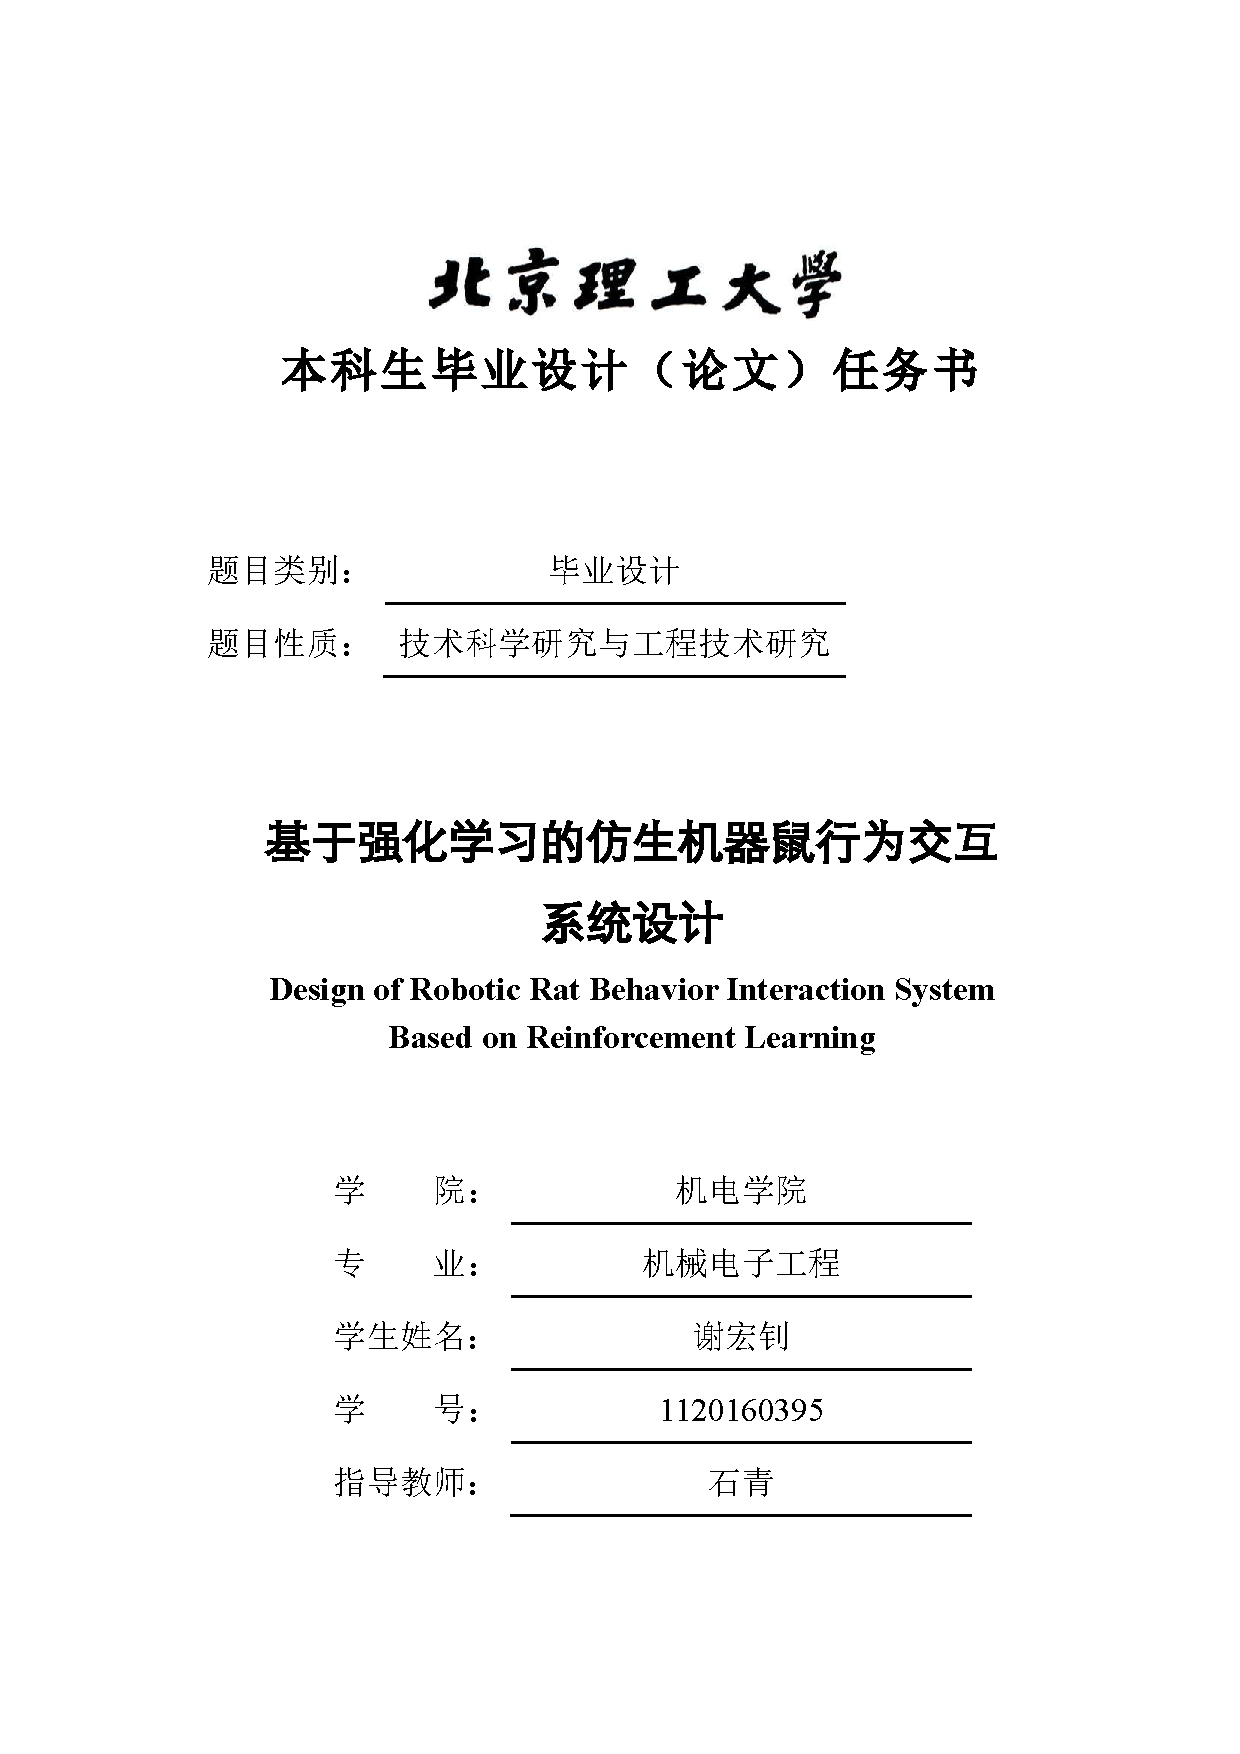
\includepdf{misc/00_worksheet1.pdf}
% 
\includepdf{misc/00_worksheet2.pdf}
% 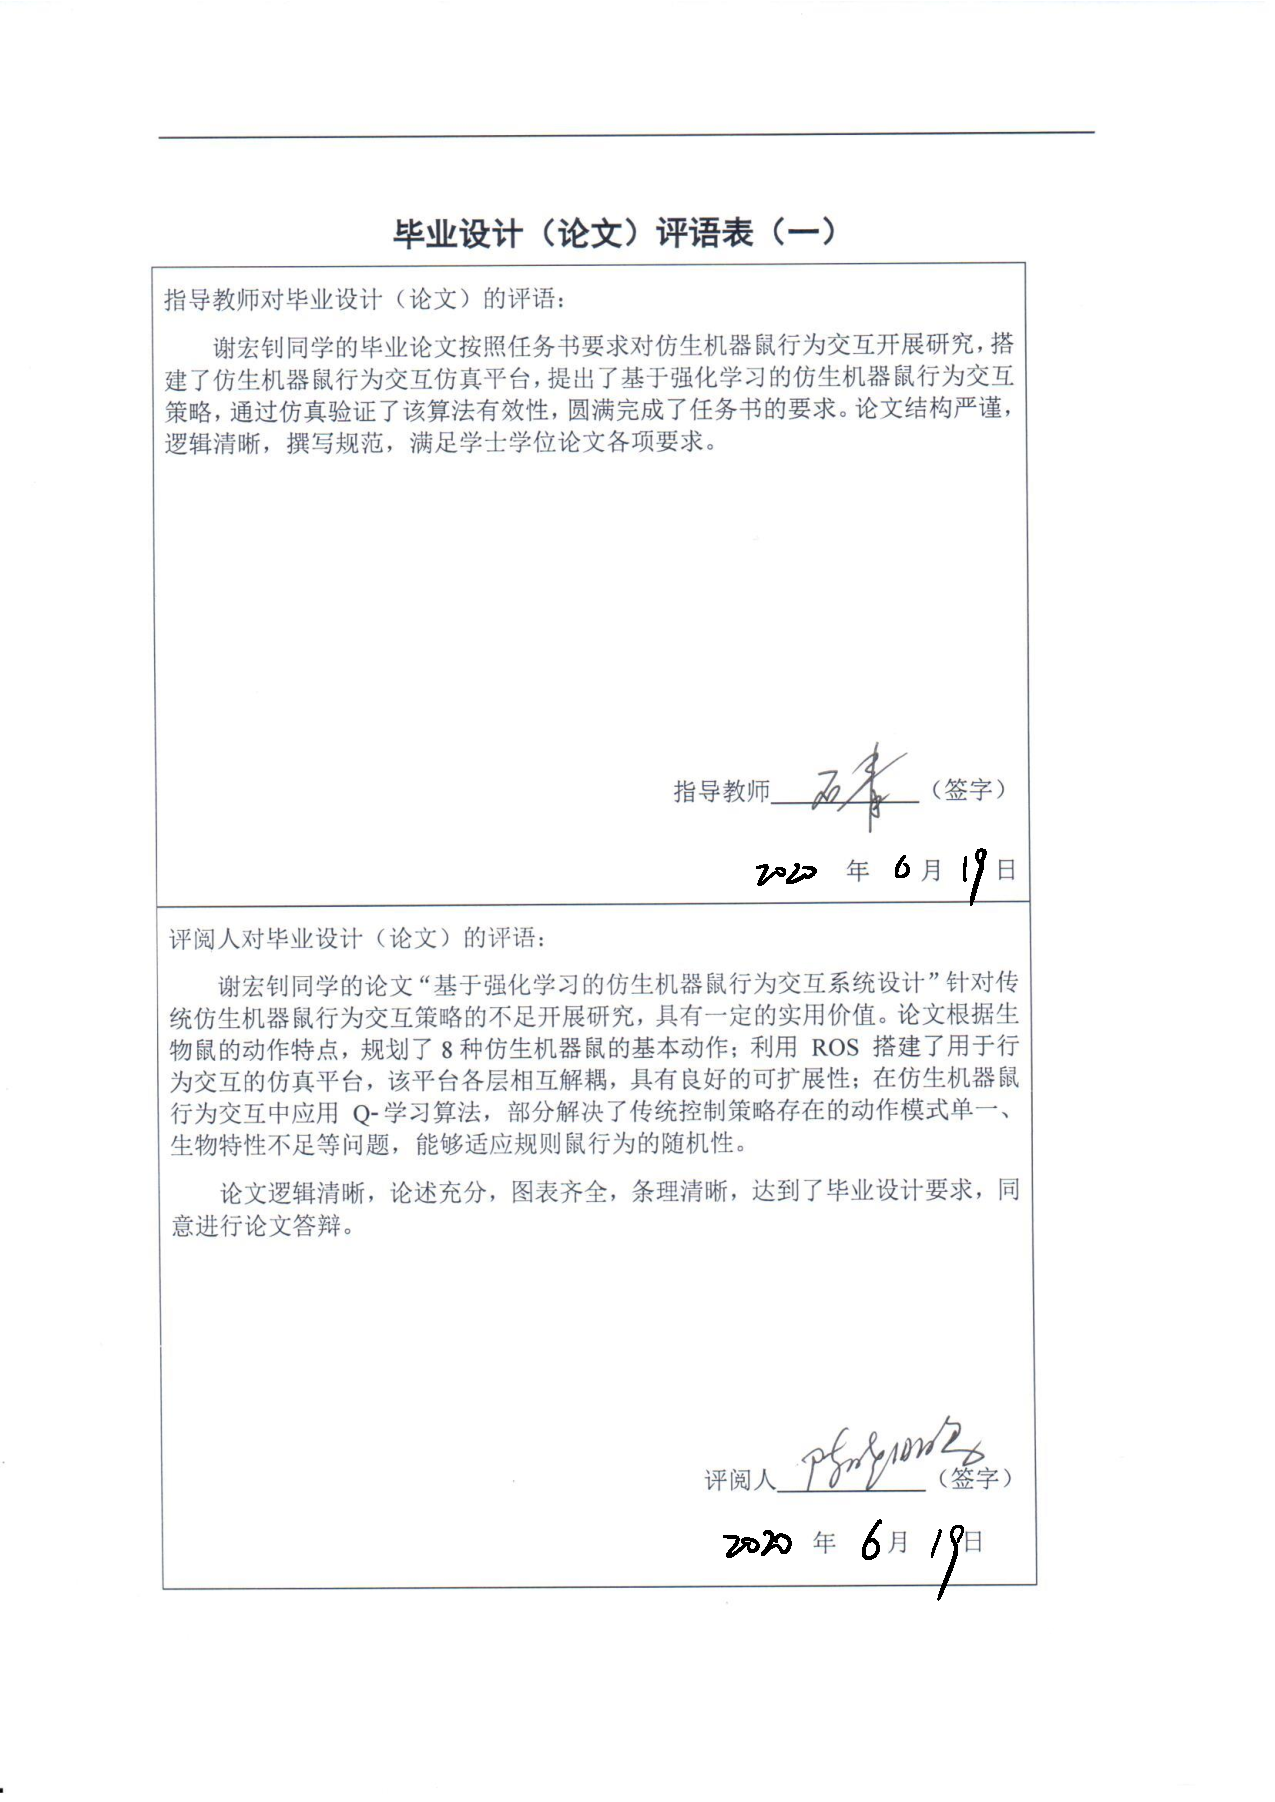
\includepdf{misc/01_comment1.pdf}
% 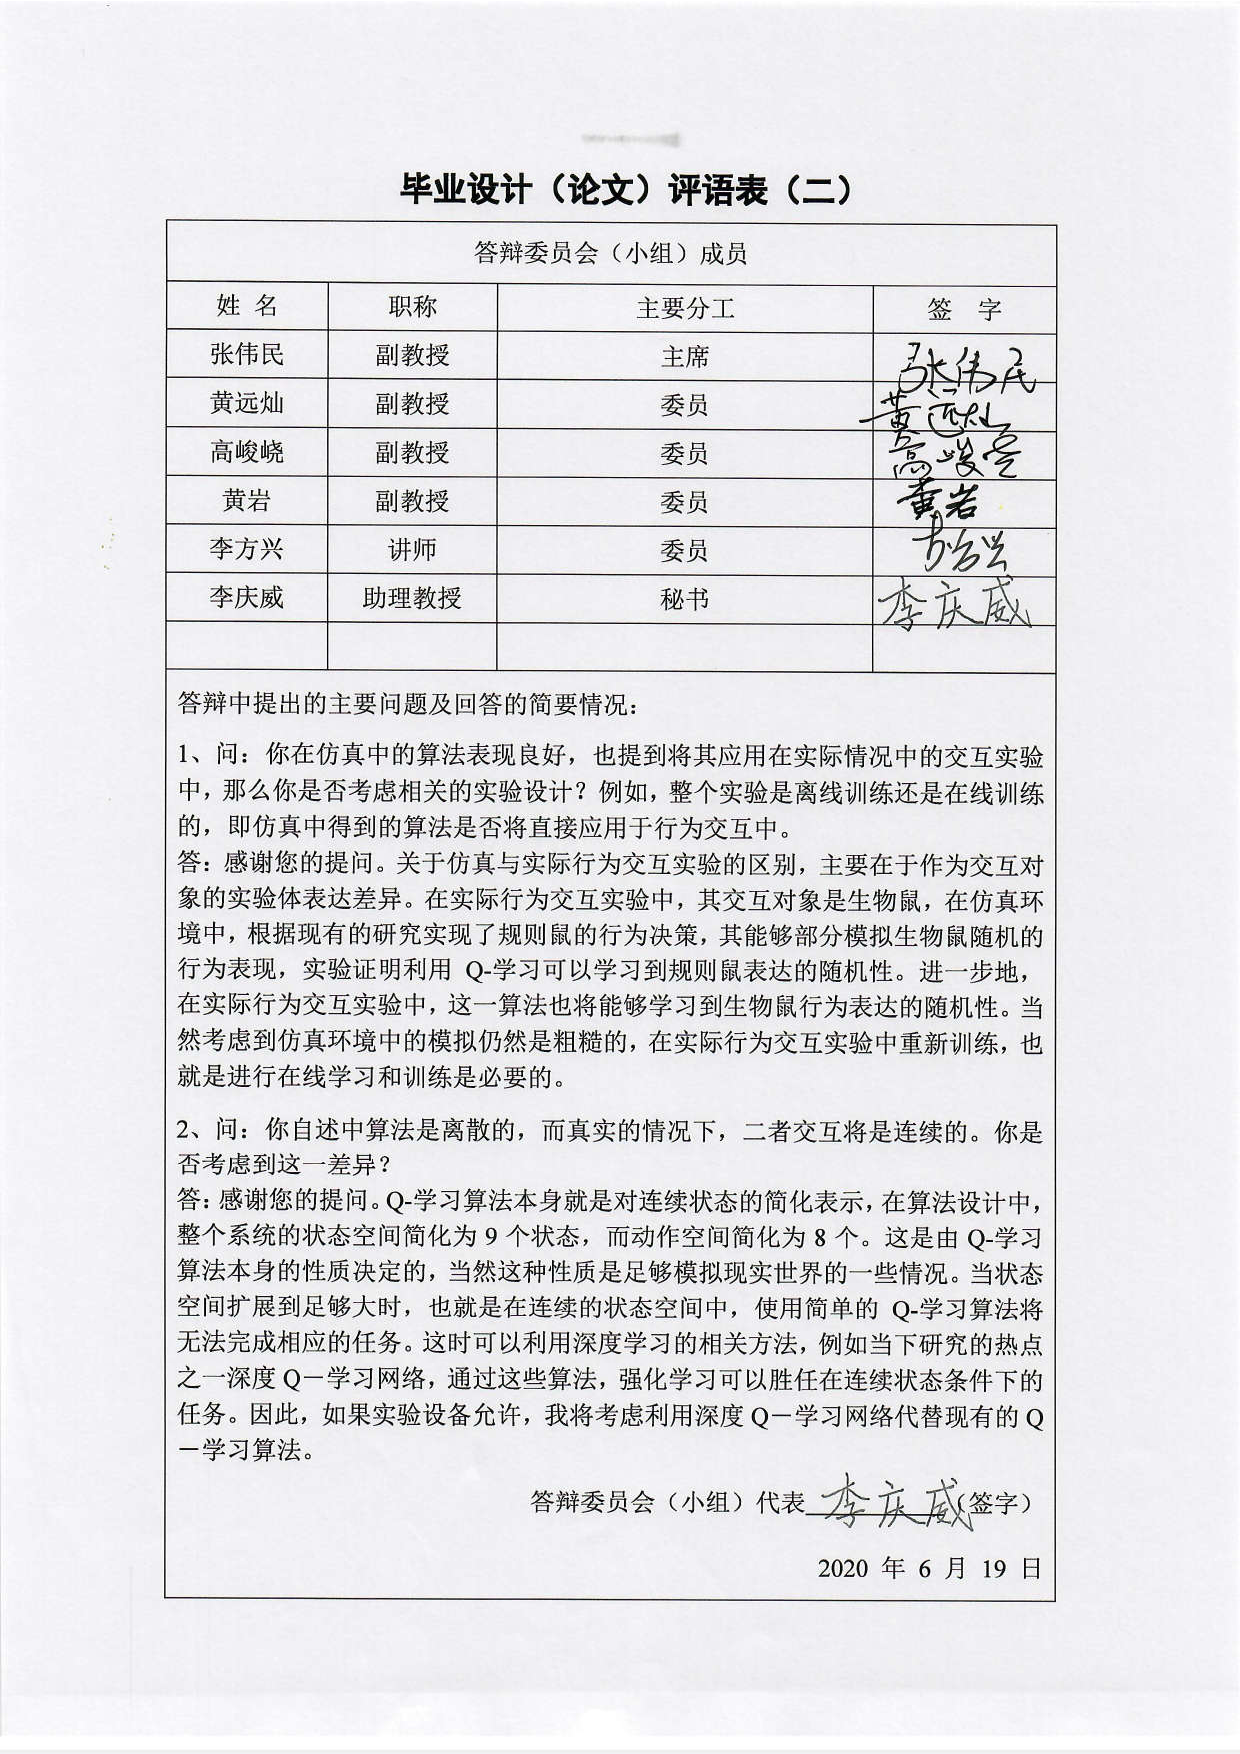
\includepdf{misc/01_comment2.pdf}
% 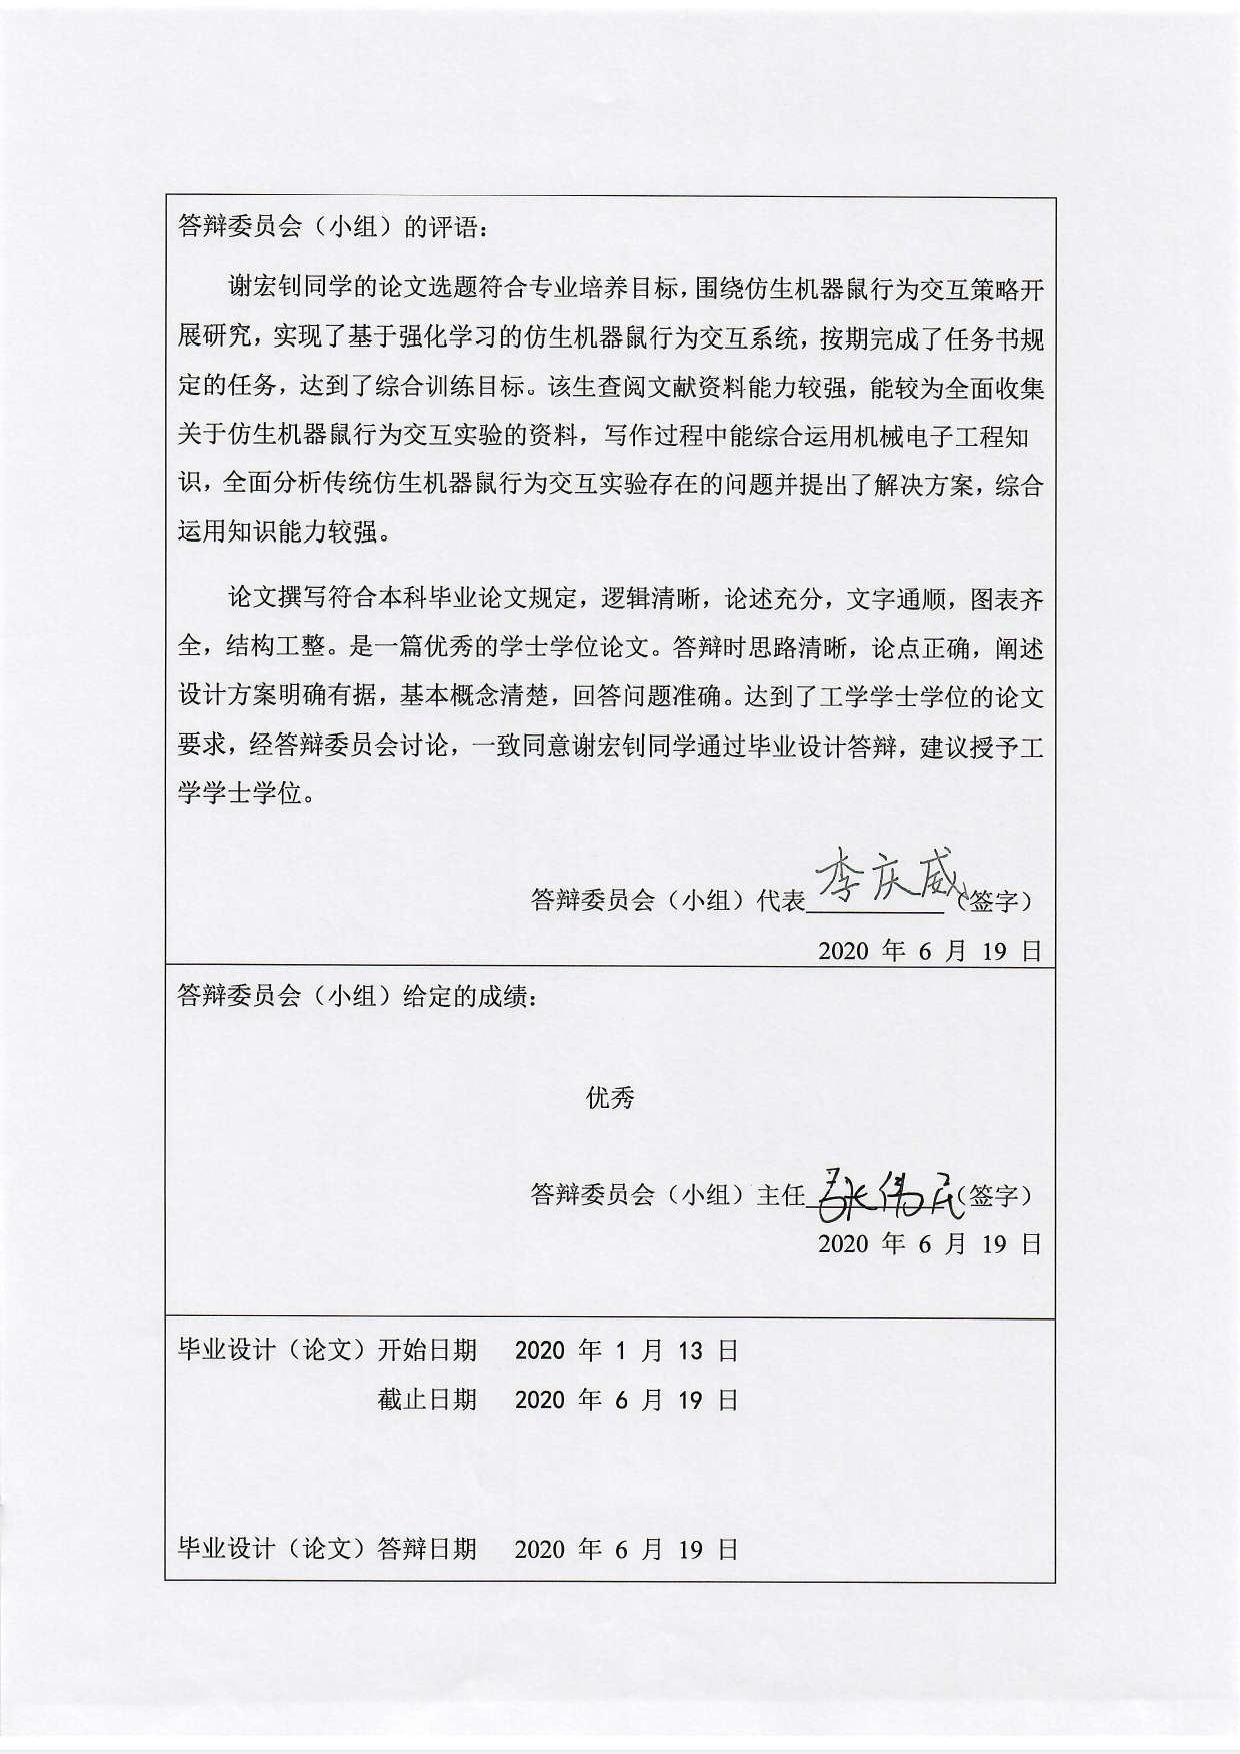
\includepdf{misc/01_comment3.pdf}
% 
\includepdf{misc/1_originality.pdf}
\newpage
%%%
% The BIThesis Template for Bachelor Graduation Thesis
%
% 北京理工大学毕业设计(论文)原创性声明页 —— 使用 XeLaTeX 编译
%
% Copyright 2020 Spencer Woo
%
% This work may be distributed and/or modified under the
% conditions of the LaTeX Project Public License, either version 1.3
% of this license or (at your option) any later version.
% The latest version of this license is in
%   http://www.latex-project.org/lppl.txt
% and version 1.3 or later is part of all distributions of LaTeX
% version 2005/12/01 or later.
%
% This work has the LPPL maintenance status `maintained'.
%
% The Current Maintainer of this work is Spencer Woo.
%
% 如无特殊需要,本页面无需更改

% 原创性声明页无页码页面格式
\fancypagestyle{originality}{
  % 页眉高度
  \setlength{\headheight}{20pt}

  % 页眉和页脚(页码)的格式设定
  \fancyhf{}
  \fancyhead[C]{\zihao{4}\ziju{0.08}\songti{北京理工大学本科生毕业设计(论文)}}

  % 页眉分割线稍微粗一些
  \renewcommand{\headrulewidth}{0.6pt}
}

\pagestyle{originality}
\topskip=0pt

% 圆形数字编号定义
\newcommand{\circled}[2][]{\tikz[baseline=(char.base)]
  {\node[shape = circle, draw, inner sep = 1pt]
  (char) {\phantom{\ifblank{#1}{#2}{#1}}};
  \node at (char.center) {\makebox[0pt][c]{#2}};}}
\robustify{\circled}

% 设置行间距
\setlength{\parskip}{0.4em}
\renewcommand{\baselinestretch}{1.41}

% 顶部空白
\vspace*{-6mm}

% 原创性声明部分
\begin{center}
  \heiti\zihao{2}\textbf{原创性声明}
\end{center}

% 本部分字号为小三
\zihao{-3}

本人郑重声明:所呈交的毕业设计(论文),是本人在指导老师的指导下独立进行研究所取得的成果。除文中已经注明引用的内容外,本文不包含任何其他个人或集体已经发表或撰写过的研究成果。对本文的研究做出重要贡献的个人和集体,均已在文中以明确方式标明。

特此申明。

\vspace{13mm}

\begin{flushright}
  本人签名:\hspace{40mm}日\hspace{2.5mm}期:\hspace{13mm}年\hspace{8mm}月\hspace{8mm}日
\end{flushright}

\vspace{17mm}

% 使用授权声明部分
\begin{center}
  \heiti\zihao{2}\textbf{关于使用授权的声明}
\end{center}

本人完全了解北京理工大学有关保管、使用毕业设计(论文)的规定,其中包括:\circled{1}学校有权保管、并向有关部门送交本毕业设计(论文)的原件与复印件;\circled{2}学校可以采用影印、缩印或其它复制手段复制并保存本毕业设计(论文);\circled{3}学校可允许本毕业设计(论文)被查阅或借阅;\circled{4}学校可以学术交流为目的,复制赠送和交换本毕业设计(论文);\circled{5}学校可以公布本毕业设计(论文)的全部或部分内容。

\vspace*{1mm}

\begin{flushright}
  \begin{spacing}{1.65}
    \zihao{-3}
    本人签名:\hspace{40mm}日\hspace{2.5mm}期:\hspace{13mm}年\hspace{8mm}月\hspace{8mm}日\\
    指导老师签名:\hspace{40mm}日\hspace{2.5mm}期:\hspace{13mm}年\hspace{8mm}月\hspace{8mm}日
  \end{spacing}
\end{flushright}

\newpage

% 摘要:在摘要相应的 TeX 文件处进行摘要部分的撰写
% %%
% The BIThesis Template for Bachelor Graduation Thesis
%
% 北京理工大学毕业设计(论文)中英文摘要 —— 使用 XeLaTeX 编译
%
% Copyright 2020 Spencer Woo
%
% This work may be distributed and/or modified under the
% conditions of the LaTeX Project Public License, either version 1.3
% of this license or (at your option) any later version.
% The latest version of this license is in
%   http://www.latex-project.org/lppl.txt
% and version 1.3 or later is part of all distributions of LaTeX
% version 2005/12/01 or later.
%
% This work has the LPPL maintenance status `maintained'.
%
% The Current Maintainer of this work is Spencer Woo.

% 中英文摘要章节
\topskip=0pt
\zihao{-4}

\vspace*{-7mm}

\begin{center}
  \heiti\zihao{-2}\textbf{\thesisTitle}
\end{center}

\vspace*{2mm}

\addcontentsline{toc}{chapter}{摘~~~~要}
{\let\clearpage\relax \chapter*{\textmd{摘~~~~要}}}
\setcounter{page}{1}

\vspace*{1mm}

\setstretch{1.53}
\setlength{\parskip}{0em}

% 中文摘要正文从这里开始
利用仿生机器人与生物开展行为交互实验,揭示生物的行为生成机制和研究仿生机器人的控制策略是智能机器人和生物学领域的热点之一。仿生机器鼠模仿生物鼠结构设计,能够引发生物鼠的特定反应,二者交互研究受到研究人员的广泛关注。当前利用仿生机器鼠行为交互主要分为示教实验和社交反应测试两类,示教实验中交互策略存在动作模式单一问题,社交反应测试中仿生机器鼠行为生成普遍缺乏生物特性。

首先,根据生物鼠动作特点及仿生机器鼠结构特性,提出了前进、后退、左转、右转、梳理、被梳理、攀爬和匍匐共8种基本动作的规划方法,解决了示教实验中动作模式单一的问题。

其次,设计并搭建了用于开展仿生机器鼠行为交互的仿真平台,该平台分为关节控制、动作执行和行为生成三个层次,各层之间相互解耦,可扩展性强,具备模拟多机器鼠在实验场景中行为交互的能力。

最后,在仿真平台中,设定强化学习控制的仿生机器鼠为学习鼠,预设规则控制的仿生机器鼠为规则鼠,利用Q-学习算法训练学习鼠适应规则鼠行为的行为模式,产生与规则鼠匹配的动作序列,实现了生物鼠行为交互过程中接近与跟随特性的模拟,增强了仿生机器鼠行为生成的生物特性。

%利用仿生机器人与生物开展行为交互实验,揭示生物的行为生成机制和研究仿生机器人的控制策略是智能机器人和生物学领域的热点之一。生物鼠作为一种典型的模式动物,对其行为交互的研究受到仿生机器鼠开发者的广泛关注。当前研究者开展的仿生机器鼠行为交互实验主要为示教实验和社交反应测试两类,在示教实验中仿生机器鼠的交互策略存在着动作模式单一的问题,而社交反应测试中仿生机器鼠行为生成方式往往缺乏生物特性。
%
%首先,针对示教实验中动作模式单一的问题,本文根据生物鼠的动作特点,结合仿生机器鼠模型都结构特性,规划前进、后退、左转、右转、梳理、被梳理、攀爬和匍匐共8种基本动作,扩展其动作空间。
%
%其次,为模拟仿生机器鼠行为交互的相关现象,设计并搭建了用于开展仿生机器鼠行为交互的仿真平台,该平台分为关节控制、动作执行和行为生成三个层次,各层之间相互解耦,可扩展性强,具备模拟多机器鼠在实验场景中行为交互的能力。
%
%最后,针对传统方法生物特性不足的问题,本文引入强化学习的思想,利用Q-学习算法训练仿生机器鼠与设定的规则鼠在仿真平台中进行行为交互,使其适应规则鼠行为的随机性。经过训练后的仿生机器鼠能够适应规则鼠的行为模式,在仿真平台中习得生物鼠行为交互时的接近与跟随特性,产生与规则鼠匹配的动作序列,表现出与生物鼠相似的行为交互模式。

%本文……。
%
%\textcolor{blue}{摘要正文选用模板中的样式所定义的“正文”,每段落首行缩进 2 个字符;或者手动设置成每段落首行缩进 2 个汉字,字体:宋体,字号:小四,行距:固定值 22 磅,间距:段前、段后均为 0 行。阅后删除此段。}
%
%\textcolor{blue}{摘要是一篇具有独立性和完整性的短文,应概括而扼要地反映出本论文的主要内容。包括研究目的、研究方法、研究结果和结论等,特别要突出研究结果和结论。中文摘要力求语言精炼准确,本科生毕业设计(论文)摘要建议 300-500 字。摘要中不可出现参考文献、图、表、化学结构式、非公知公用的符号和术语。英文摘要与中文摘要的内容应一致。阅后删除此段。}

\vspace{4ex}\noindent\textbf{\heiti 关键词:仿生机器鼠;行为交互;强化学习;ROS}
\newpage

% 英文摘要章节
\topskip=0pt

\vspace*{2mm}

\begin{spacing}{0.95}
  \centering
  \heiti\zihao{3}\textbf{\thesisTitleEN}
\end{spacing}

\vspace*{17mm}

\addcontentsline{toc}{chapter}{Abstract}
{\let\clearpage\relax \chapter*{
  \zihao{-3}\textmd{Abstract}\vskip -3bp}}
\setcounter{page}{2}

\setstretch{1.53}
\setlength{\parskip}{0em}
% 英文摘要正文从这里开始
%It is one of the hotspots in the field of intelligent robots and biology to take advantage of bionic robot to conduct social interaction test with living counterparts, which can help reveal behavior generation mechanisms in creatures and improve control strategies of bionic robot. Rats, as model animals, have been widely concerned by the researchers in robotic rat. Current strategies proposed by researchers to control the robotic rat in social interaction test generally are weak in interaction ability, continuance and adaptability.
%
%Aiming to overcome such weakness, I have made an action planning of the robotic rat, so that it can produce basic movements similar to the biological rat. A simulation system for robotic rat in social interaction test has been established, which is able to simulate the behavioral interaction of multi-robots in experimental scenarios. To solve the problem of uncontinuance and poor adaptability, Q-learning has been used to generate the action sequence of the robotic rat in social interaction test, and trained with the rule-based rat in the simulation system.
%
%As a result, Q-learning-based robotic rat is able adapt to the behavior of its partner, and shows a behavior interaction mode similar to that of the living rat in the simulation system. The continuance and adaptability of the control strategy have been improved.

It is one of the hotspots in the field of intelligent robots and biology to take advantage of bionic robot interacting with living counterparts, revealing behavior mechanisms in creatures and improving control strategies of bionic robot. The robotic rat imitating the structural of the living rat, are capable of triggering specific reflex of the living rat. Thus interaction experiments between the two has attracted attention from researchers. At present, there are two typical areas: teaching and social reaction test. In the teaching, the control strategy are weak in action modes. In the social reaction test, the behavioral generation of the robotic rat generally lacks biological characteristics.

First of all, according to the characteristics of the living rat and the structural of the robotic rat, a total of 8 basic movement planning methods of forward, backward, left turning, right turning, grooming, groomed, climbing and creeping were proposed, which extends action modes.

Secondly, a simulation platform for simulating behavioral interaction between the robotic rat was established, which was divided into three layers: joint control layer, motion execution layer and behavior generation layer. Each layer, with strong scalability, decoupled from each other, were able to simulate behavioral interaction in experimental scenarios.

Finally, in the simulation platform, the robotic rat controlled by reinforcement learning is defined as the learning rat, and the rule-controlled robotic rat as the rule rat. the learning rat was trained by the Q-learning to adapt to the behavior mode of the rule rat, generate the matching action sequence. As a result, this strategy simulated approaching and following characteristics in the interaction process, and enhanced the biological characteristics of the robotic rat.

\vspace{3ex}\noindent\textbf{Key Words: Robotic Rat; Behavior Interaction; Reinforcement Learning; ROS}
\newpage

% 目录:如无特殊需要,本部分无需改动
% %%
% The BIThesis Template for Bachelor Graduation Thesis
%
% 北京理工大学毕业设计(论文)目录 —— 使用 XeLaTeX 编译
%
% Copyright 2020 Spencer Woo
%
% This work may be distributed and/or modified under the
% conditions of the LaTeX Project Public License, either version 1.3
% of this license or (at your option) any later version.
% The latest version of this license is in
%   http://www.latex-project.org/lppl.txt
% and version 1.3 or later is part of all distributions of LaTeX
% version 2005/12/01 or later.
%
% This work has the LPPL maintenance status `maintained'.
%
% The Current Maintainer of this work is Spencer Woo.
%
% 如无特殊需要,本页面无需更改

% 目录开始

% 调整目录行间距
\renewcommand{\baselinestretch}{1.35}
% 目录
\tableofcontents
\newpage


% 正文开始
\mainmatter
% 正文 22 磅的行距
\setlength{\parskip}{0em}
\renewcommand{\baselinestretch}{1.53}

% 第一章
%%
% The BIThesis Template for Bachelor Graduation Thesis
%
% 北京理工大学毕业设计(论文)第一章节 —— 使用 XeLaTeX 编译
%
% Copyright 2020 Spencer Woo
%
% This work may be distributed and/or modified under the
% conditions of the LaTeX Project Public License, either version 1.3
% of this license or (at your option) any later version.
% The latest version of this license is in
%   http://www.latex-project.org/lppl.txt
% and version 1.3 or later is part of all distributions of LaTeX
% version 2005/12/01 or later.
%
% This work has the LPPL maintenance status `maintained'.
%
% The Current Maintainer of this work is Spencer Woo.
%
% 第一章节

\chapter{绪论}
% \section{课题研究背景与意义}
仿生机器人是机器人研究的一大分支,旨在通过研究生物系统的结构、性状、原理、行为以及相互作用,从而为机器人设计、控制和决策提供新的设计思想、工作原理和系统构成\cite{sunFangShengXueDeXianZhuangHeWeiLai2007},是一门集生命科学、物质科学、数学与力学、信息科学、工程技术以及系统科学等学科的交叉学科\cite{wangFangShengJiQiRenYanJiuXianZhuangYuFaZhanQuShi2015}。生物体结构合理,运动灵活,具有良好的环境适应特性和良好的生存能力,仿生机器人因其部分模仿生物结构和性状特点而继承了一部分这些特性,受到研究者的青睐\cite{shenFangShengJiQiRenYanJiuJinZhanJiFangShengJiGouYanJiu2015}。生物鼠是被广泛使用的实验动物之一\cite{kongShiYanDongWuPinXiShuJuKuDeJianLi2015},对其行为模式的研究收到生物学家的广泛关注,但由于生物鼠行为随机、难以预测,相关的实验开展存在困难。作为仿生机器人的一个基本实例,设计精巧的仿生机器鼠可以模拟生物鼠各个关节的运动,从而产生与生物鼠相似的基本行为,并以此引发生物鼠的特异性反应\cite{gaoOverviewBiomimeticRobots2019}。因此,利用仿生机器鼠与生物鼠进行行为交互,探究交互过程中生物鼠的反应与仿生机器鼠行为的联系,对研究生物鼠的行为模式和机器人的控制策略均有重要意义\cite{frohnwieserUsingRobotsUnderstand2016}。

但在实践中,仿生机器鼠与生物鼠的行为交互仍然面临诸多困难。首先,两者交互时行为的一致性有赖于双方,特别是仿生机器鼠反应的快速性\cite{kleinRobotsServiceAnimal2012}。而生物鼠身体构造精巧,动作灵活,反应机敏,模仿其身体特点设计的仿生机器鼠往往具有复杂的结构和较多的自由度,给仿生机器鼠的动作规划带来了挑战。在产生仿鼠动作过程中,仿生机器鼠的控制系统往往需要耗费大量时间计算正、逆运动学问题,使得仿生机器鼠反应迟钝,难以满足交互实验的需求。其次,生物鼠行为表现具有普遍的个体差异\cite{BarnettSTheRat},这导致难以用特定的方法对其行为加以预测或控制,给仿生机器鼠的行为生成方式提出了挑战。单一机制的行为生成算法在经过调试后,往往只能适用于某一特定的生物鼠,当切换交互对象后,相应的算法往往需要进行调整,实验的可重复性大大降低。最后,生物鼠在实验环境中往往表现出渐进的环境适应性,这意味着同一生物鼠在实验之初和实验进行一段时间后表现出的行为模式存在较明显的差异。而单一的仿生机器鼠行为生成机制无法适应生物鼠的这一行为变化,这导致了部分控制策略在初期表现优秀,但随着时间推移,其可用性往往大不如前。上述现实困难使得现有的机器鼠与生物鼠的交互实验存在着可重复性差、应用场景单一和持续时间较短等不足。

% 随着人工智能领域相关技术的发展,研究者开始关注其在仿生机器鼠与生物鼠行为交互领域的作用。典型应用包括利用深度神经网络识别生物鼠的行为模式,为仿生机器鼠的行为决策提供依据,这一应用使得仿生机器鼠具有了处理大量交互数据的能力\cite{dechaumontComputerizedVideoAnalysis2012a},但仍未对其行为生成机制产生重大影响。强化学习是机器学习中的一个领域,强调如何基于环境而行动,以取得最大化的预期利益\cite{liuShenDuQiangHuaXueXiZongShu2018}。其灵感来源于心理学中的行为主义理论,即有机体如何在环境给予的奖励或惩罚的刺激下,逐步形成对刺激的预期,产生能获得最大利益的习惯性行为。近来,基于强化学习控制的机器人在Atari游戏、围棋和德州扑克等领域表现优异,其中DeepMind的AlphaGo机器人击败围棋冠军李世石成为大众关注的热点\cite{silverMasteringGameGo2017, botvinickReinforcementLearningFast2019}。考虑到仿生机器鼠与生物鼠交互过程与Atari游戏等具有高度的相似性,利用强化学习训练机器人完成复杂环境中的任务受到人工智能和机器人领域研究者的重视。
% \section{国内外研究现状}
\subsection{仿生机器鼠研究现状}
生物鼠形体轻巧,行动灵活,表现出优秀的地形适应能力,激发了研究者开发仿生多足移动机器人的灵感。但由于早期研究者设计四足仿生机器鼠时面临着驱动器和控制器集成、小型机器人四足步态规划等难题,较早成熟的仿生机器鼠大多为轮式结构。其中以日本早稻田大学Takanishi实验室开发的WM(Waseda Mouse)系列仿生机器鼠(图\ref{figure_wm})较为典型。
\begin{figure}[htbp]
  %\vspace{10pt} % 调整图片与上文的垂直距离
  \centering
  \subfigure[WM-2\cite{takanishiInteractionCreatureRobot1998}]{
  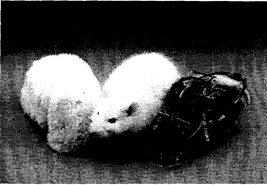
\includegraphics[height=0.18\linewidth]{images/ch01/WM2.png} \label{figure_wm2}% label 用来在文中索引
  }
  \subfigure[WM-4\cite{aokiInteractionRatRatrobots1999}]{
  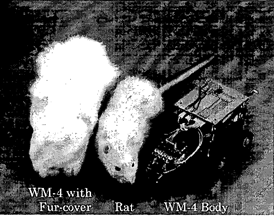
\includegraphics[height=0.18\linewidth]{images/ch01/WM4.png} \label{figure_wm4}% label 用来在文中索引
  }
  \subfigure[WM-6\cite{ishiiExperimentalStudyAutomatic2005}]{
  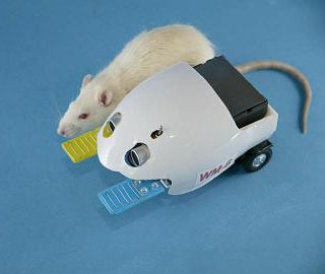
\includegraphics[height=0.18\linewidth]{images/ch01/WM6.jpg} \label{figure_wm6}% label 用来在文中索引
  }
  \subfigure[WM-8\cite{ishiiStressExposureUsing2012}]{
  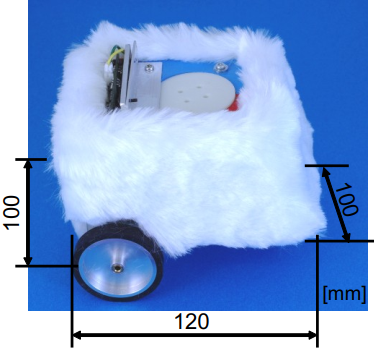
\includegraphics[height=0.18\linewidth]{images/ch01/WM8.png} \label{figure_wm8}% label 用来在文中索引
  }
  \caption{部分WM系列仿生机器鼠} \label{figure_wm}
\end{figure}
这一系列仿生机器鼠尺寸均与成年鼠相近,装备有红外传感器用于探测生物鼠和其他环境障碍,具备两个后置的驱动轮,使用者可以通过蓝牙对其运动进行控制\cite*{takanishiInteractionCreatureRobot1998, aokiInteractionRatRatrobots1999,  ishiiExperimentalStudyAutomatic2005, ishiiStressExposureUsing2012}。WM-2型仿生机器鼠由两个前置的转向轮控制方向,而随后WM-4型仿生机器鼠对两个驱动轮分别控制,使其能够进行差速运动,进而实现任意线速度和角速度的运动,这不仅提高了改型仿生机器鼠的灵活性,而且使得原本用于转向的前轮改为仅需提供支撑的万向轮,简化了仿生机器鼠的结构\cite{aokiInteractionRatRatrobots1999}。在后续的研究中,他们更新了WM-6的驱动器,并改进了外形,新的WM-8型仿生机器鼠在最大角速度上大幅超过WM-6,并且外形与生物鼠更相似\cite{ishiiStressExposureUsing2012}。

近年来,随着电机和控制器的小型化,将其集成在小型移动机器平台上成为可能。同时,人们对生物鼠的运动机理揭示逐渐深入,为仿生机器鼠的设计提供了思路。近年来,四足仿生机器鼠成为热点之一。日本和意大利的研究者们共同开发的一款仿生机器鼠全身具有12个自由度\cite{laschiDesignDevelopmentLegged2006a},能够执行前进、转向、推动杠杆和按下按钮等简单的动作,但由于其采用钢丝-滑轮驱动,运动精度较低。而日本早稻田大学自2009年开始其四足仿生机器鼠WR(Waseda Rat)系列(图\ref{figure_wr})的研究。
\begin{figure}[htbp]
  %\vspace{13pt} % 调整图片与上文的垂直距离
  \centering
  \subfigure[WR-1\cite{ishiiDevelopmentQuadrupedAnimaroid2009}]{
  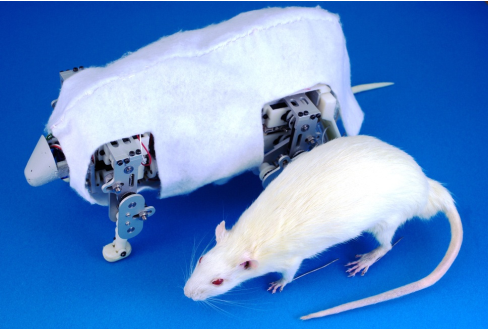
\includegraphics[height=0.2\linewidth]{images/ch01/WR1.png} \label{figure_wr1}
  }
  \subfigure[WR-2\cite{ishiiDesignDevelopmentBiomimetic2009}]{
  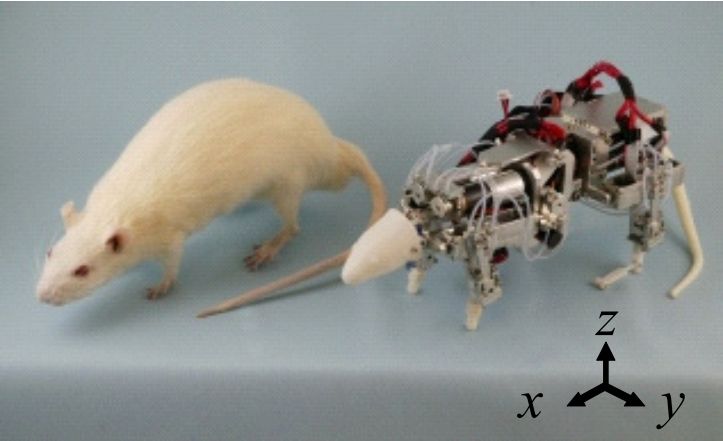
\includegraphics[height=0.2\linewidth]{images/ch01/WR2.png} \label{figure_wr2}
  }\\
  \subfigure[WR-3\cite{shiDevelopmentHybridWheellegged2010, shiDevelopmentHybridWheelLegged2011, ishiiNovelMethodDevelop2013}]{
  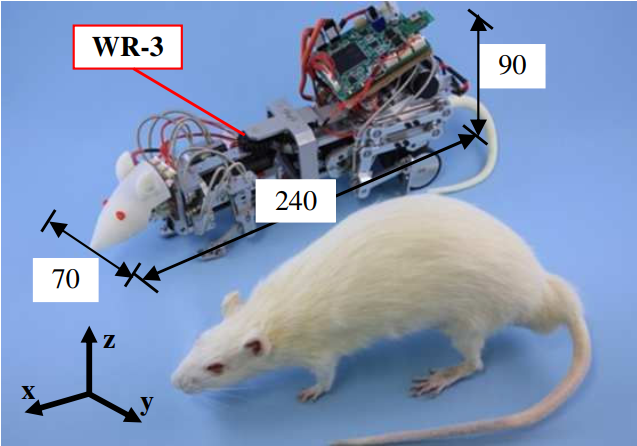
\includegraphics[height=0.2\linewidth]{images/ch01/WR3.png} \label{figure_wr3}
  }
  \subfigure[WR-4\cite{shiRobotratInteractionExperimental2011a}]{
  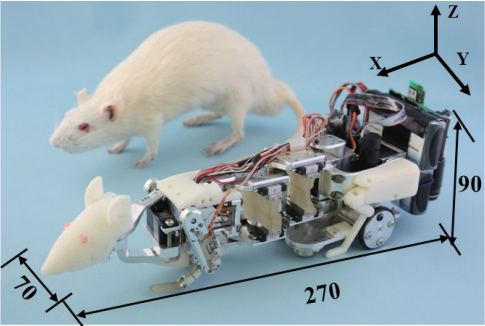
\includegraphics[height=0.2\linewidth]{images/ch01/WR4.png} \label{figure_wr4}
  }
  \subfigure[WR-5\cite{shiBehaviorModulationRats2015a}]{
  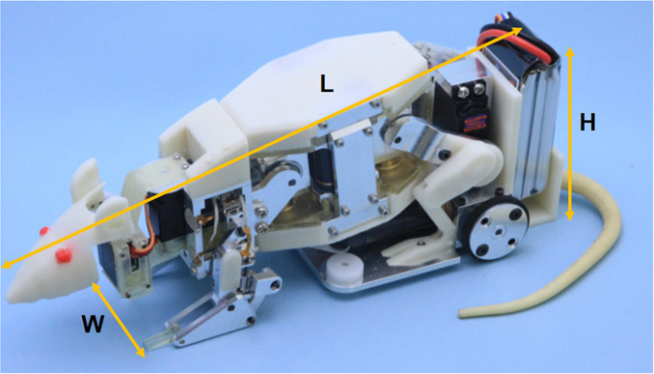
\includegraphics[height=0.2\linewidth]{images/ch01/WR5.png} \label{figure_wr5}
  }
  \caption{WR系列仿生机器鼠} \label{figure_wr}
\end{figure}
该系列仿生机器鼠每条腿均有2个主动自由度和1个被动自由度\cite*{ishiiDevelopmentQuadrupedAnimaroid2009, ishiiDesignDevelopmentBiomimetic2009, shiDevelopmentHybridWheellegged2010, shiRobotratInteractionExperimental2011a, shiDevelopmentHybridWheelLegged2011, ishiiNovelMethodDevelop2013, shiBehaviorModulationRats2015a},尽管WR-1和WR-2在产生仿鼠动作方面有不俗的表现,可以执行部分生物间交互动作,但由于其质量均远超生物鼠(约为其3倍),且运动性能不佳,最大速度仅为2-3 cm/s\cite*{ishiiDevelopmentQuadrupedAnimaroid2009, ishiiDesignDevelopmentBiomimetic2009},因此其交互性能受到局限。与前两代相比,WR-3采用轮-腿复合结构,不仅对尺寸进行了优化,还对前肢结构进行了设计,能够完成梳理等典型生物鼠动作\cite{shiDevelopmentHybridWheellegged2010},该型号仿生机器鼠在仿鼠运动方面取得了较大的发展。其后的WR-4仿生机器鼠共有12个主动自由度,运动更加灵活。在此基础上,WR-5针对仿生机器鼠的外形进行了改进,并针对腰部连接进行了模块化设计,WR-5重0.8 kg,具有13个自由度,大大提升了模仿生物鼠动作的能力\cite{shiBehaviorModulationRats2015a}。随着对生物鼠运动机理的进一步揭示,研究人员在WR-5的基础上进行了改进,根据生物鼠的运动情况设置仿生机器鼠的自由度,改进后的WR-5M在俯仰、偏向等运动模式方面均表现出与生物鼠相近的性质\cite{shiModifiedRoboticRat2018}。

除WR系列仿生机器鼠外,德国慕尼黑工业大学也对仿生机器鼠进行了研究。其开发的NRP系列仿生机器鼠(图\ref{figure_tum})利用弹簧机构模拟生物鼠腿部肌腱,实现仿鼠行走运动\cite{lucasDesignBiomimeticRodent2018}。
\begin{figure}[htbp]
  %\vspace{0pt} % 调整图片与上文的垂直距离
  \centering
  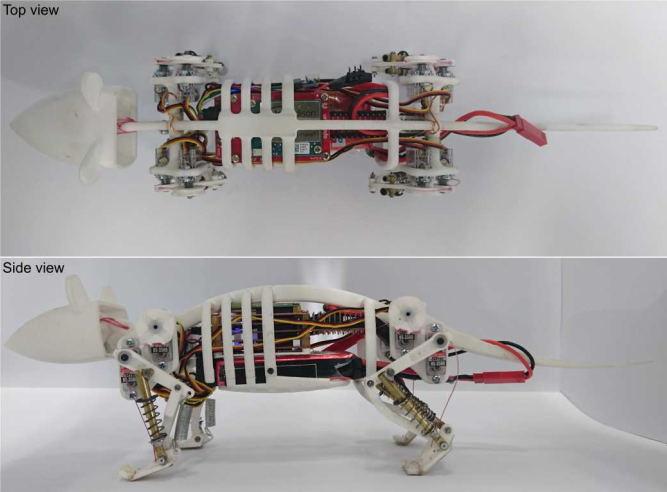
\includegraphics[width=0.5\linewidth]{images/ch01/tum.png}
  \caption{慕尼黑工业大学仿生机器鼠}\label{figure_tum} % label 用来在文中索引
\end{figure}

对仿生机器鼠腰部结构的设计是另一难点。一般认为,生物鼠腰部对其实现前身俯仰和偏航运动具有重要作用,因此必须具备至少2个自由度\cite{shiDevelopmentHybridWheellegged2010},早期的仿生机器鼠均不具备腰部运动的能力\cite{ishiiStressExposureUsing2012, ishiiDesignDevelopmentBiomimetic2009, ishiiDevelopmentQuadrupedAnimaroid2009, shiModulationRatBehaviour2013},限制着仿生机器鼠产生仿鼠运动,这一情况到2009年得以改善,早稻田大学的研究人员设计的WR-3仿生机器鼠具备2个腰部自由度,但这一设计为其腿部运动的稳定性,尤其是产生直立动作时带来了挑战,为克服这一困难,他们采取了轮-腿复合结构,并在WR-4中沿用这一设计\cite{shiDevelopmentHybridWheellegged2010, shiRobotratInteractionExperimental2011a, shiDevelopmentHybridWheelLegged2011}。而NRP系列仿生机器鼠采用弹簧四肢结构和鼠尾辅助支撑实现直立动作,因此未设置腰部自由度,这也使得其转弯半径高达30-40 cm,灵活度较差\cite{lucasDesignBiomimeticRodent2018}。

国内仿生机器鼠设计也有一定成果。东北大学设计的四轮仿生机器鼠(图\ref{figure_cn}\subref{figure_nerat})具有一定的在筛网状地面行走和进入小洞的能力,但并不具备任何生物鼠特有的动作特性\cite{guoFangShengShuJiJieXiTongSheJiYuYunDongTeXingYanJiu2010}。徐若愚等设计的机械小鼠(图\ref{figure_cn}\subref{figure_xurat})通过添加一系列感应装置实现仿鼠行为,包括觅食、逃避和自我保护等\cite{xuFangShengJiJieXiaoShuDeYanJiuJiSheJi2016}。我们对日本早稻田大学的WR-5仿生机器鼠进行了改进得到WR-5M(图\ref{figure_cn}\subref{figure_lirat}),优化设计了前肢机构及控制电路板,使得该仿生机器鼠在外形上更接近生物鼠,同时能够更好地模仿生物鼠的前肢运动,在最大俯仰角(MPA)和最大到达高度(MRH)、最大弯曲角(MBA)和最小弯曲距离(MBD)4个参数的评估中均有较大改善\cite{liJiQiShuDeFangShuYunDongChengDuPingGu2017a}。
\begin{figure}[htbp]
  %\vspace{13pt} % 调整图片与上文的垂直距离
  \centering
  \subfigure[东北大学四轮仿生机器鼠\cite{guoFangShengShuJiJieXiTongSheJiYuYunDongTeXingYanJiu2010}]{
  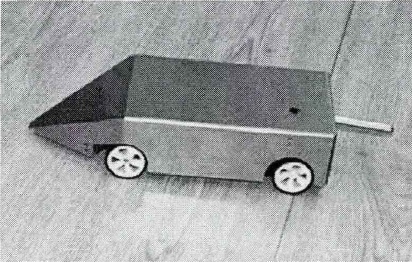
\includegraphics[height=0.18\linewidth]{images/ch01/nerat.png} \label{figure_nerat}
  }
  \subfigure[徐若愚机械小鼠\cite{xuFangShengJiJieXiaoShuDeYanJiuJiSheJi2016}]{
  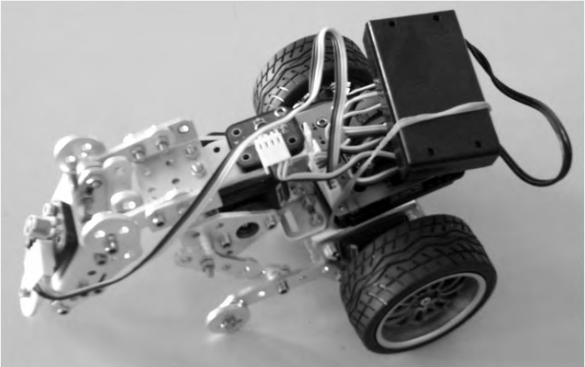
\includegraphics[height=0.18\linewidth]{images/ch01/xurat.png} \label{figure_xurat}
  }
  \subfigure[WR-5M仿生机器鼠\cite{liJiQiShuDeFangShuYunDongChengDuPingGu2017a}]{
  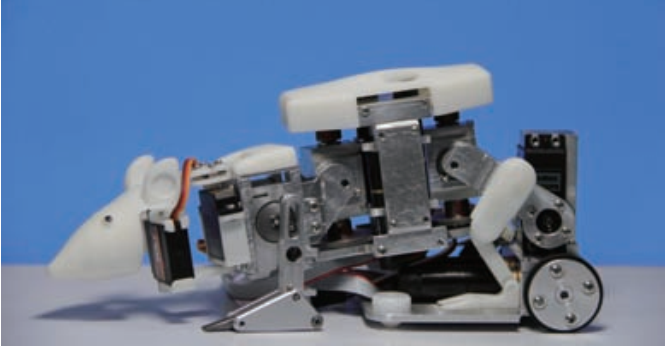
\includegraphics[height=0.18\linewidth]{images/ch01/lirat.png} \label{figure_lirat}
  }
  \caption{国内仿生机器鼠研究} \label{figure_cn}
\end{figure}

综合以上研究,目前仿生机器鼠经历了从轮式到足式,从腰部固连到设置多个腰部自由度的过程,其发展具有明显的小型化和智能化的趋势,与生物鼠的外形差距在不断减小。随着对生物鼠机理的进一步揭示,仿生机器鼠结构和运动将得到不断优化,其行为产生、智能控制和决策领域将受到研究者进一步重视,而仿生机器鼠与生物鼠的行为交互即是这一领域的重要研究方向。

\subsection{仿生机器鼠交互研究}
作为一种典型的模式动物,生物鼠的行为表现与其内部情绪变化、个体生理属性即外部环境状态有着密切联系。揭示生物鼠行为变化,尤其是多只生物鼠交互时的变化规律,对揭示其上述生物特性有着重要意义,因而受到研究者的广泛关注。但由于生物的不可控性,在研究过程中,科学家一直试图寻找一种便于操控的仪器作为生物鼠的交互对象。仿生机器鼠的出现为此提供了一种选择,设计精巧的仿生机器鼠皆能够产生与生物鼠相似的动作和行为,进而诱发生物鼠的交互反应,又能够被科学家精确控制。在研究仿生机器鼠结构和控制方式的过程中,研究者们也一直在关注其在动物交互实验过程中的作用。

WM系列仿生机器鼠的研究团队利用其成果进行了部分社交试验。他们利用WM-2研究仿生机器鼠对生物鼠行为的影响,在实验的前半部分,生物鼠对仿生机器鼠表现出经常性的嗅探和跟随行为;随着实验进行,生物鼠表现出与仿生机器鼠齐头并进的行为,这表明仿生机器鼠的部分行为能够被生物鼠认知并影响生物鼠的行为\cite{takanishiInteractionCreatureRobot1998}。但这一实验只研究了距离这一单一变量,且其焦点为生物鼠与仿生机器鼠之间的信息交流,因而对内部的生物机理揭示不足。
随后,他们利用WM-4型仿生机器鼠研究其是否能够引导生物鼠的某些行为,在实验中,WM-4与生物鼠同时寻找食物,当仿生机器鼠寻找到食物后,主动引导生物鼠前往食物位置。实验发现,当WM-4重复这一引导行为后,生物鼠受到影响,跟随WM-4并找到食物\cite{aokiInteractionRatRatrobots1999}。除此以外,\citeauthor{ishiiExperimentalStudyTask2006}提出了一种新的算法策略(图\ref{figure_wminteract}\subref{figure_wm6teach})对WM-6的接近、推杆等动作进行了训练,结果发现这一算法能够有效地对生物鼠的觅食行为进行示教\cite{ishiiExperimentalStudyTask2006}。而随后利用WM-8进行的对生物鼠的压力测试(图\ref{figure_wminteract}\subref{figure_stressEx})发现未成年生物鼠在遭受仿生机器鼠的压力时表现出比成年生物鼠更低的活力\cite{ishiiStressExposureUsing2012},这也表明仿生机器鼠可以作为研究生物鼠精神状态的良好工具。
\begin{figure}[htbp]
  %\vspace{13pt} % 调整图片与上文的垂直距离
  \centering
  \subfigure[WM-6仿生机器鼠行为生成算法\cite{ishiiExperimentalStudyTask2006}]{
  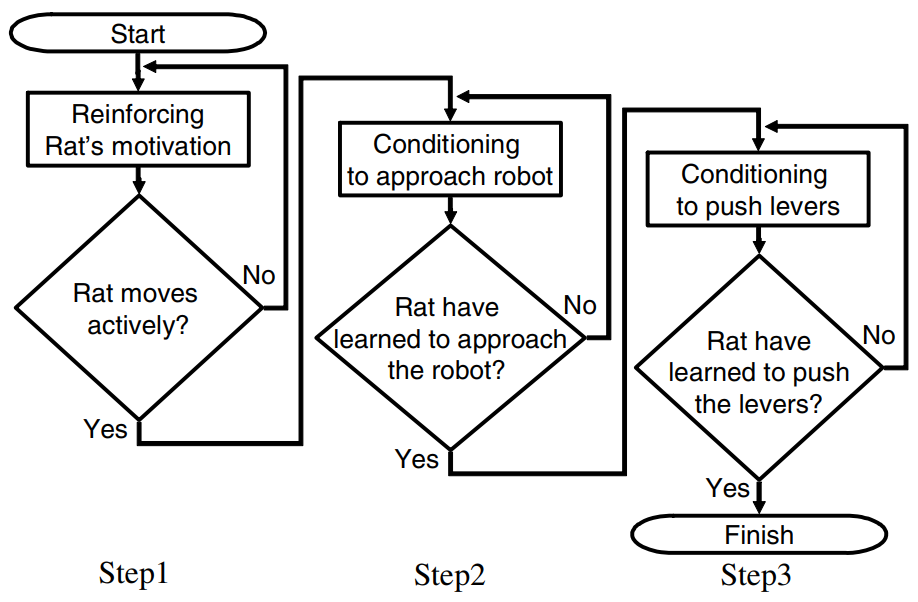
\includegraphics[height=0.3\linewidth]{images/ch01/WM6teach.png} \label{figure_wm6teach}
  }
  \subfigure[WM-8对生物鼠进行压力测试的实验装置\cite{ishiiStressExposureUsing2012}]{
  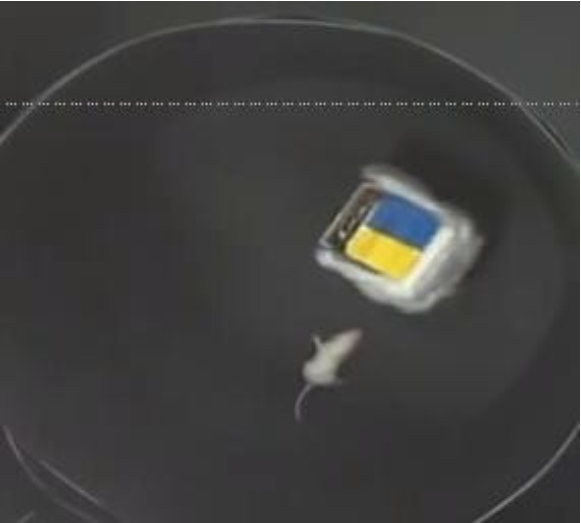
\includegraphics[height=0.3\linewidth]{images/ch01/StressEx.png} \label{figure_stressEx}
  }
  \caption{部分WM系列仿生机器鼠行为交互实验} \label{figure_wminteract}
\end{figure}

研究人员同样利用WR仿生机器鼠开展了一系列交互实验,\citeyear{laschiDesignDevelopmentLegged2006a}年,
开发团队尝试利用四足仿生机器鼠示教生物鼠执行特定的动作后获取食物\cite{laschiDesignDevelopmentLegged2006a}。WR-3具有优秀的产生仿鼠运动的能力,他们将生物鼠的运动阶段分为移动和交互两个过程,控制仿生机器鼠产生直立、转身、梳理和爬上等行为,在交互实验中生物鼠对仿生机器鼠由戒备逐渐变为友好,这表明仿生机器鼠的特定社交行为能够诱使生物鼠模仿其行为。\cite{shiDevelopmentHybridWheellegged2010}。

随后,他们利用WR-4与生物鼠进行了社交反应测试,在实验中,WR-4在第一阶段表现跟随行为(5 $min$),之后不再运动(5 $min$),将第二阶段生物鼠表现直立行为的频率和与WR-4的距离作为观测结果,发现与WR-4交互后,生物鼠表现直立的频率明显提高,表明WR-4能够明显地影响生物鼠的行为\cite{shiRobotratInteractionExperimental2011a}。这一结论随后由WR-5M得到了证实,当WR-5M表现出与生物鼠相似的俯仰和偏向动作时,生物鼠通常随之表现出一致的动作(图\ref{figure_wr5minter}),表明机器鼠具有欺骗生物鼠并诱使其产生特定行为的能力\cite{shiModifiedRoboticRat2018}。但这些实验往往存在着持续时间短,交互模式单一等问题。
\begin{figure}[htbp]
  %\vspace{13pt} % 调整图片与上文的垂直距离
  \centering
  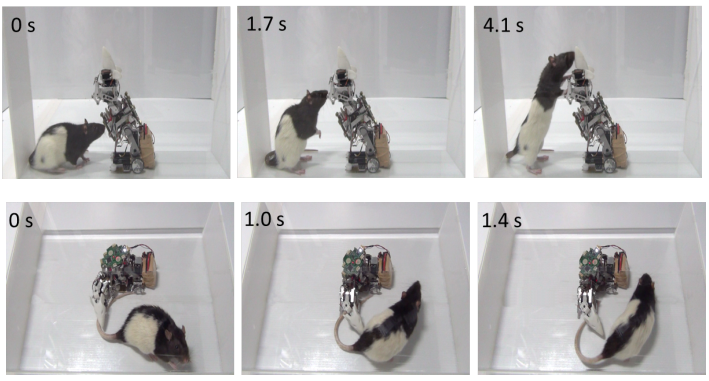
\includegraphics[width=0.6\linewidth]{images/ch01/wr-5minter}
  \caption{WR-5M与生物鼠交互\cite{shiModifiedRoboticRat2018}}\label{figure_wr5minter}
\end{figure}

在社交反应测试中,仿生机器鼠与生物鼠的距离作为一个重要变量受到研究者关注,因而便于控制速度的轮式机器人受到青睐。除早期的WM系列仿生机器鼠外,近来研究者利用与生物鼠尺寸相似的轮式机器人进行了一些研究。\citeauthor{delangelortizSocialInteractionTest2016}利用外形与生物鼠相差较大的e-puck机器人进行社交反应测试(图\ref{figure_epuck}),通过比较生物鼠与机器人和生物鼠与另一生物鼠交互的不同行为表现,发现e-puck机器人能够抑制生物鼠的活动性\cite{delangelortizSocialInteractionTest2016}。
\begin{figure}[htb]
  %\vspace{13pt} % 调整图片与上文的垂直距离
  \centering
  \subfigure[接近1]{
  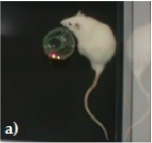
\includegraphics[width=0.17\linewidth, height=0.18\linewidth]{images/ch01/epuck/a.png} \label{figure_epuck_a}
  }
  \subfigure[接近2]{
  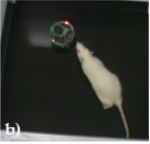
\includegraphics[width=0.17\linewidth, height=0.18\linewidth]{images/ch01/epuck/b.png} \label{figure_epuck_b}
  }
  \subfigure[嗅探]{
  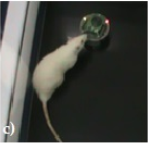
\includegraphics[width=0.17\linewidth, height=0.18\linewidth]{images/ch01/epuck/c.png} \label{figure_epuck_c}
  }
  \subfigure[跟随1]{
  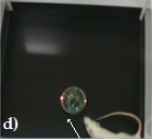
\includegraphics[width=0.17\linewidth, height=0.18\linewidth]{images/ch01/epuck/d.png} \label{figure_epuck_d}
  }
  \subfigure[跟随2]{
  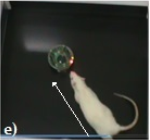
\includegraphics[width=0.17\linewidth, height=0.18\linewidth]{images/ch01/epuck/e.png} \label{figure_epuck_e}
  }\\
  \subfigure[跟随3]{
  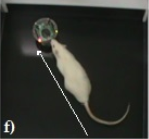
\includegraphics[width=0.17\linewidth, height=0.18\linewidth]{images/ch01/epuck/f.png} \label{figure_epuck_f}
  }
  \subfigure[攀爬]{
  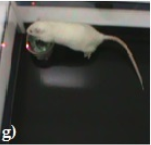
\includegraphics[width=0.17\linewidth, height=0.18\linewidth]{images/ch01/epuck/g.png} \label{figure_epuck_g}
  }
  \subfigure[梳理]{
  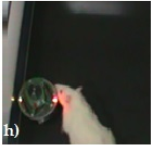
\includegraphics[width=0.17\linewidth, height=0.18\linewidth]{images/ch01/epuck/h.png} \label{figure_epuck_h}
  }
  \subfigure[自梳理]{
  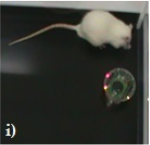
\includegraphics[width=0.17\linewidth, height=0.18\linewidth]{images/ch01/epuck/i.png} \label{figure_epuck_i}
  }
  \subfigure[躲避1]{
  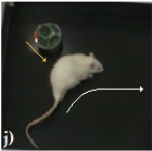
\includegraphics[width=0.17\linewidth, height=0.18\linewidth]{images/ch01/epuck/j.png} \label{figure_epuck_j}
  }\\
  \subfigure[躲避2]{
  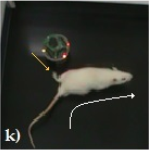
\includegraphics[width=0.17\linewidth, height=0.18\linewidth]{images/ch01/epuck/k.png} \label{figure_epuck_k}
  }
  \subfigure[探索1]{
  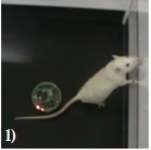
\includegraphics[width=0.17\linewidth, height=0.18\linewidth]{images/ch01/epuck/l.png} \label{figure_epuck_l}
  }
  \subfigure[探索2]{
  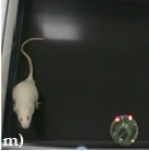
\includegraphics[width=0.17\linewidth, height=0.18\linewidth]{images/ch01/epuck/m.png} \label{figure_epuck_m}
  }
  \subfigure[不移动]{
  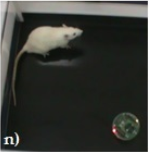
\includegraphics[width=0.17\linewidth, height=0.18\linewidth]{images/ch01/epuck/n.png} \label{figure_epuck_n}
  }
  \subfigure[镇定]{
  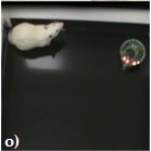
\includegraphics[width=0.17\linewidth, height=0.18\linewidth]{images/ch01/epuck/o.png} \label{figure_epuck_o}
  }
  \caption{e-puck机器人与生物鼠交互\cite{delangelortizSocialInteractionTest2016}} \label{figure_epuck}
\end{figure}

昆士兰大学的研究人员提出了一种利用轮式仿生机器鼠PiRat与生物鼠行为交互的闭环控制框架,实验中,生物鼠的运动轨迹作为PiRat控制系统的输入量,据此决定PiRat是否接近生物鼠,这一设定将生物鼠的状态作为系统输入,使得该系统具有了一定的适应性,但由于将机器鼠的动作划分为接近和远离两种模式,并未能较彻底地揭示生物鼠行为交互机理(图\ref{figure_pirat_interact})\cite{heathPiRatAutonomousFramework2018}。
\begin{figure}[htb]
  %\vspace{13pt} % 调整图片与上文的垂直距离
  \centering
  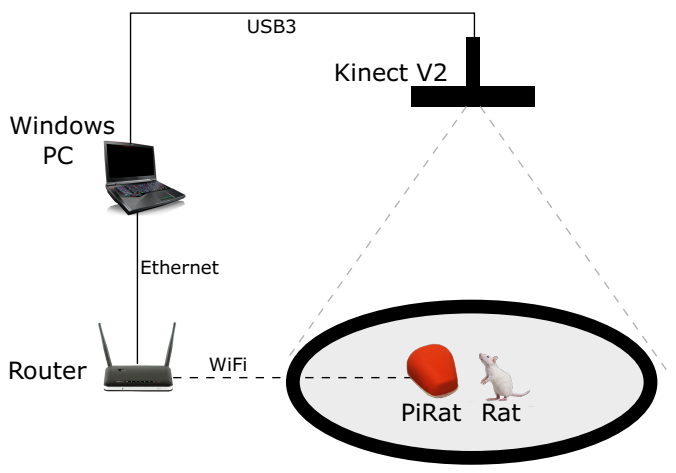
\includegraphics[width=0.5\linewidth]{images/ch01/piratintera.png}
  \caption{PiRat与生物鼠交互实验装置\cite{heathPiRatAutonomousFramework2018}}\label{figure_pirat_interact}
\end{figure}

此外还有\citeauthor{quinnWhenRatsRescue2018}研究当仿生机器鼠受困时,生物鼠是否会营救仿生机器鼠。他们利用仿生机器鼠产生“有作用”或者“无作用”的动作,并将其关入笼中,随后发现生物鼠会营救仿生机器鼠,并且倾向于营救“有作用的”仿生机器鼠(图\ref{figure_rescure})\cite{quinnWhenRatsRescue2018}。

国内对生物鼠与机器鼠的行为交互仍处于起步阶段,但利用强化学习和马尔可夫决策过程进行人机交互的训练已经得到应用。北京科技大学的\citeauthor{wangJiYuFangRenJiQiRenDeRenJiJiaoHuYuHeZuoYanJiu2015}构建了一种基于情感推理的多Agent情感决策模型,并基于情感能量理论,建立起基于HMM(Hidden Markov Model)的心境状态调节算法,该算法对于不完全和确定性知识具备较为准确的推理能力\cite{wangJiYuFangRenJiQiRenDeRenJiJiaoHuYuHeZuoYanJiu2015}。

综合以上研究,目前开展的生物鼠与仿生机器鼠行为交互实验主要聚焦于三个方面。第一,通过探究生物鼠对仿生机器鼠的反应,与对生物鼠的反应作比较,验证仿生机器鼠设计的合理性。第二,通过控制仿生机器鼠产生特定的仿鼠动作,诱使生物鼠模拟和跟随仿生机器鼠的动作,作为控制生物鼠行为的途径。第三,将仿生机器鼠的动作作为生物鼠的外部刺激,观察生物鼠对特定刺激做出的反应,研究生物鼠行为模式与外部刺激的关系。而上述三个方面均缺乏对两者长期交互的关注,使得现有研究无法适应生物鼠存在的随机性。为使机器人具备高级的社交能力,必须令其能够从所处环境中学习相关经验和知识\cite{bhaumikAIRobotics2018}。强化学习的基本思想是为代理设定学习目标,使其感知环境状态并作出决策,直到达成相应的目标\cite{ISI:000481873900002}。这一特性使得强化学习有助于解决仿生机器鼠与生物鼠交互时存在的随机性问题。
% \section{研究目标}
\begin{enumerate}[leftmargin=0em, label=(\theenumi)]
%\setlength{\leftmargin}{0em}
\setlength{\itemindent}{4em}
\setlength{\labelsep}{0em}
\setlength{\labelwidth}{2em}
\setlength{\parsep}{0em}
\setlength{\itemsep}{0em}
\setlength{\topsep}{0em}
%\begin{enumerate}[leftmargin=0em, listparindent=2em, parsep=0em, topsep=0em, label=(\theenumi)]
%\setlength{\itemindent}{4em}
%\setlength{\labelsep}{0em}
%\setlength{\labelwidth}{2em}
%\setlength{\parsep}{0em}
%\setlength{\itemsep}{0em}
%\setlength{\topsep}{0em}
  \item 为满足行为交互实验过程中仿生机器鼠动作实时性和快速性要求,观察生物鼠在实验场景中的典型动作,提取其在交互行为中的动作特点,并据此设计、规划仿生机器鼠的仿鼠动作。
  \item 为满足交互实验仿真需求,利用计算机系统搭建一套仿生机器鼠行为交互实验的专用仿真平台,完成仿生机器鼠仿鼠行为驱动程序编写。\label{item_target_2}
  \item 针对生物鼠行为的快速性、个体差异及其对环境渐进适应的特性,提出一套基于强化学习的仿生机器鼠行为控制方法,使机器鼠与生物鼠进行有效交互,并利用\ref{item_target_2}中搭建的仿真平台进行验证。
\end{enumerate}

\begin{figure}[htbp]
  %\vspace{13pt} % 调整图片与上文的垂直距离
  \centering
  \subfigure[机器鼠营救被困的生物鼠]{
  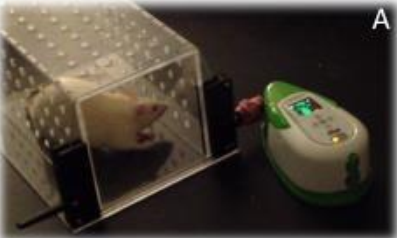
\includegraphics[width=0.4\linewidth, height=0.18\linewidth]{images/ch01/rescure/a.png} \label{figure_rescure_a}
  }
  \subfigure[生物鼠嗅探机器鼠]{
  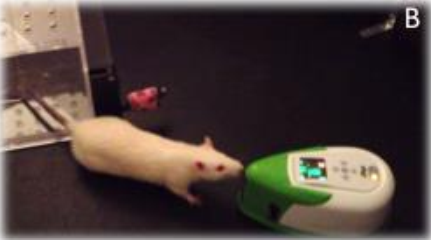
\includegraphics[width=0.35\linewidth, height=0.18\linewidth]{images/ch01/rescure/b.png} \label{figure_rescure_b}
  }
  \subfigure[生物鼠发现机器鼠被困]{
  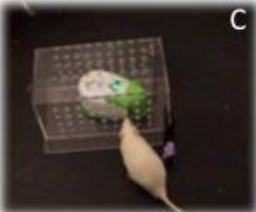
\includegraphics[width=0.23\linewidth, height=0.18\linewidth]{images/ch01/rescure/c.png} \label{figure_rescure_c}
  }
  \subfigure[生物鼠走向机关]{
  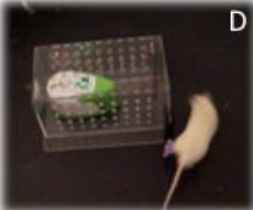
\includegraphics[width=0.23\linewidth, height=0.18\linewidth]{images/ch01/rescure/d.png} \label{figure_rescure_d}
  }
  \subfigure[生物鼠按下机关]{
  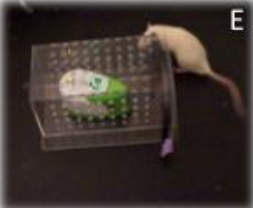
\includegraphics[width=0.23\linewidth, height=0.18\linewidth]{images/ch01/rescure/e.png} \label{figure_rescure_e}
  }
  \subfigure[生物鼠与机器鼠在笼中交互]{
  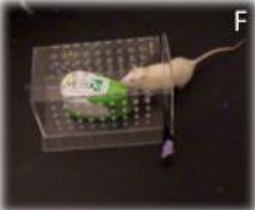
\includegraphics[width=0.23\linewidth, height=0.18\linewidth]{images/ch01/rescure/f.png} \label{figure_rescure_f}
  }
  \caption{生物鼠营救被困的“有作用的”机器鼠\cite{quinnWhenRatsRescue2018}}\label{figure_rescure}
\end{figure} 


% 在这里添加第二章、第三章……TeX 文件的引用
%%
% The BIThesis Template for Bachelor Graduation Thesis
%
% 北京理工大学毕业设计(论文)第一章节 —— 使用 XeLaTeX 编译
%
% Copyright 2020 Spencer Woo
%
% This work may be distributed and/or modified under the
% conditions of the LaTeX Project Public License, either version 1.3
% of this license or (at your option) any later version.
% The latest version of this license is in
%   http://www.latex-project.org/lppl.txt
% and version 1.3 or later is part of all distributions of LaTeX
% version 2005/12/01 or later.
%
% This work has the LPPL maintenance status `maintained'.
%
% The Current Maintainer of this work is Spencer Woo.
%
% 第二章节

\chapter{仿生机器鼠及其动作规划}
\section{仿生机器鼠模型}
经过数十年的研究,现有的仿生机器鼠模型在尺寸和结构上已与生物鼠相近,且能够产生绝大数多数与生物鼠相似的交互行为,这为本文的研究提供了坚实的基础。我们设计并优化的仿生机器鼠(后称机器鼠模型,图\ref{figure_ratbot})具有优异的产生仿鼠运动的能力\cite{liDesignOptimizationLightweight2020},本文将利用这一模型开展研究。该模型的主要特点包括:
\begin{figure}[htbp]
  %\vspace{13pt}
  \centering
  \subfigure[机器鼠模型]{
  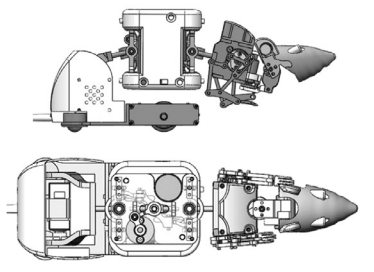
\includegraphics[width=0.45\linewidth]{images/ch02/ratbot.png} \label{figure_ratbot_model}
  }
  \subfigure[腰部机构]{
  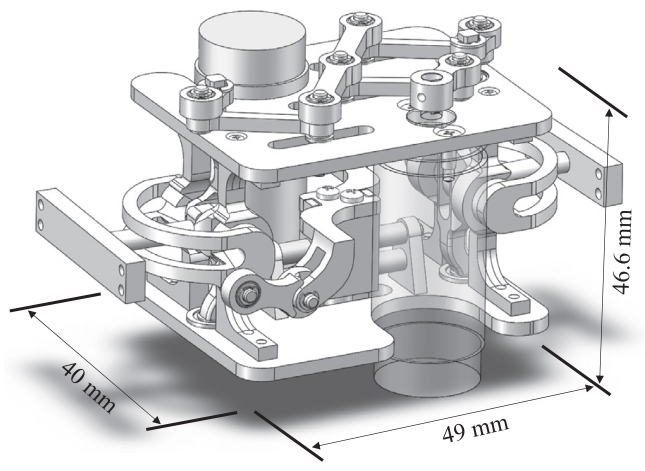
\includegraphics[width=0.45\linewidth]{images/ch02/compact-waist.png} \label{figure_ratbot_waist}
  }
  \caption{机器鼠模型及其腰部机构\cite{liDesignOptimizationLightweight2020}}\label{figure_ratbot} % label 用来在文中索引
\end{figure}
\begin{enumerate}[leftmargin=0em, topsep=0em, label=(\theenumi)]
%\setlength{\leftmargin}{0em}
\setlength{\itemindent}{4em}
\setlength{\labelsep}{0em}
\setlength{\labelwidth}{2em}
\setlength{\parsep}{0em}
\setlength{\itemsep}{0em}
\setlength{\topsep}{0em}
  \item 轮式驱动。
  \item 腰部灵活。
  \item 质量较小,运动灵活。
\end{enumerate}

此外,机器鼠模型躯干部分拥有7个主动自由度,其头颈部活动范围广,响应速度快,能够执行嗅探、探索等高频动作。是较为理想的开展行为交互实验的媒介。其部分关键属性与生物鼠比较如表\ref{table_spec}所示。
\begin{table}[htbp]
  \linespread{1.5}
  \zihao{5}
  \centering
  \caption{方式机器鼠关键属性}\label{table_spec}
  \begin{tabular}{*{3}{>{\centering\arraybackslash}m{1.5cm}}*{3}{>{\centering\arraybackslash}m{2.5cm}}}
    \toprule
    质量 & 体长 & 体宽 & 初始姿态高度    & 自由度数目 & 最大速度 \\ \midrule
    $400~g$&$195~mm$&$56~mm$&$74~mm$&$11$&$1.5~ms$\\
    \bottomrule
    \end{tabular}
\end{table}

% \section{仿生机器鼠正运动学}
机器鼠模型具有11个主动自由度,其配置情况如图\ref{figure_kinematic}\subref{figure_dof}。除轮部运动外,机器鼠的动作规划主要涉及其中的臀部、腰部和头部的7个关节,相应的坐标系统如图\ref{figure_kinematic}\subref{figure_dhframe}。
\begin{figure}[htbp]
  %\vspace{13pt}
  \centering
  \subfigure[自由度配置\cite{liDesignOptimizationLightweight2020}]{
  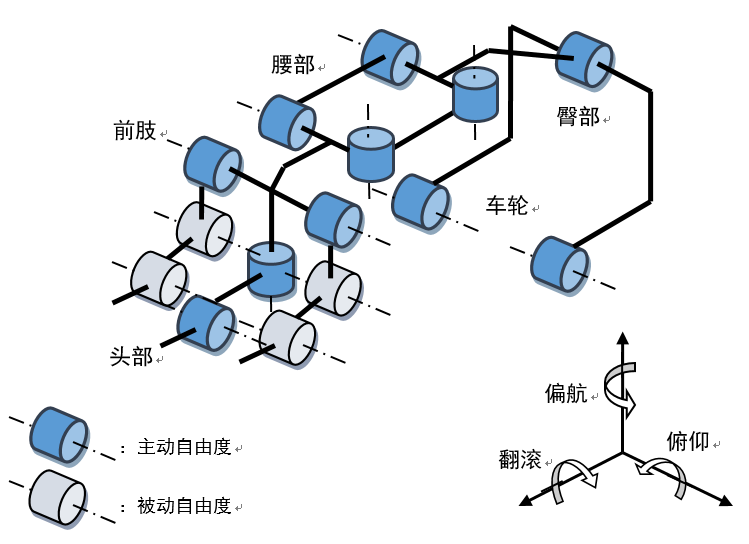
\includegraphics[height=0.21\linewidth]{images/ch02/dof.png} \label{figure_dof}
  }
  \subfigure[坐标系统\cite{liMotionEvaluation2017}]{
  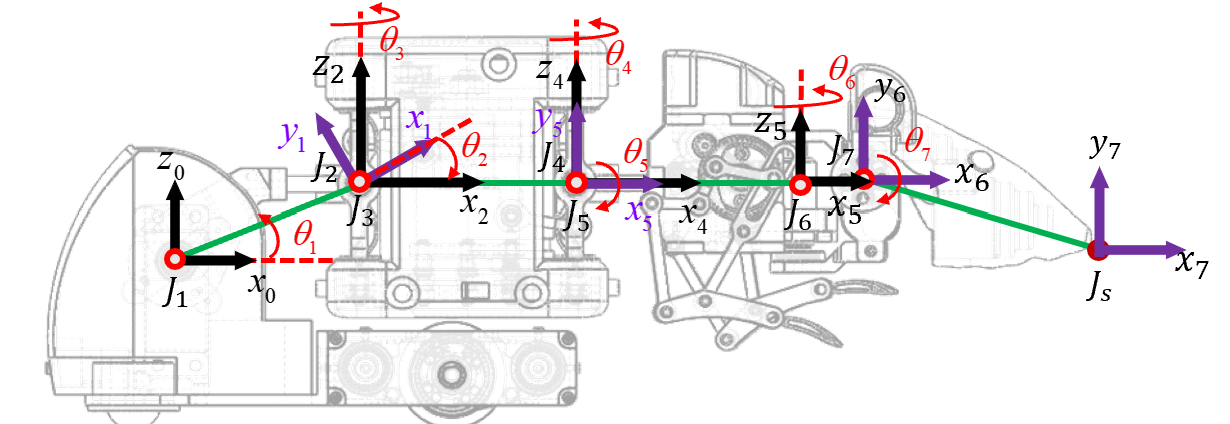
\includegraphics[height=0.21\linewidth]{images/ch02/dhframe.png} \label{figure_dhframe}
  }
  \caption{机器鼠模型自由度配置情况及其坐标系统}\label{figure_kinematic} % label 用来在文中索引
\end{figure}

七自由度机械臂的逆运动学求解是一大难点,在机械臂结构设计非特殊的情况下,通过迭代方法求得数值解是其通用解法\cite{shimizuAnalyticalInverseKinematic2008}。而考虑到数值解需要一定的计算时间,而这与实时行为交互所需的快速性相违背,因此通过正运动学计算设计特定的动作,直接控制其关节位置,而不是通过逆运动学求得关节位置,将能够显著降低程序计算时间,并提高行为交互的实时性。
%\begin{figure}[htbp]
%  \vspace{13pt}
%  \centering
%  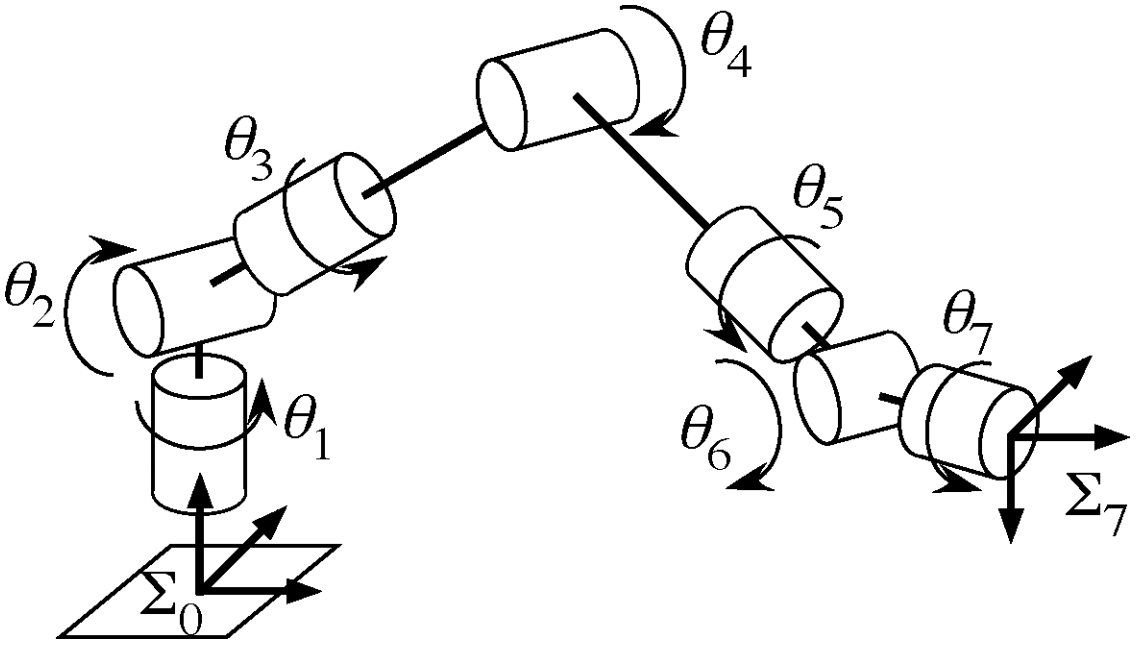
\includegraphics[width=0.6\linewidth]{images/ch02/7dof.png}
%  \caption{S-R-S构型七自由度机械臂\cite{shimizuAnalyticalInverseKinematic2008}}\label{figure_7dof}
%\end{figure}

对生物鼠而言,头部既是其重要的感知和决策部位,包括视觉、听觉和嗅觉等多种主要感觉器官和大脑这一神经中枢;又是其重要的动作执行器,几乎全部动作都需要头部的参与,并且其嘴、鼻等重要的动作执行器官也位于这一区域。因此,保证机器鼠头部的工作空间与生物鼠相同,能够为其产生仿鼠动作提供必要条件。

计算仿生机器鼠头部工作空间属于机器人正运动学的范畴,通过列写相邻关节的变换矩阵获得。根据图\ref{figure_dhframe},可以建立机器鼠躯干部分的D-H连杆参数表为表\ref{table_dh}。
\begin{table}[htbp]
  \linespread{1.5}
  \zihao{5}
  \centering
  \caption{机器鼠躯干部分D-H参数表}\label{table_dh}
  \begin{tabular}{*{5}{>{\centering\arraybackslash}p{2cm}}}
    \toprule
    $i$ & $\theta_i$ & $\alpha_{i-1}~(deg)$ & $d_i~(m)$ & $a_{i-1}~(m)$ \\ \midrule
    1   & $\theta_1$ & 0   & 0 & 0.058 \\
    2   & $\theta_2$ & -90 & 0 & 0     \\
    3   & $\theta_3$ & 0   & 0 & 0.033 \\
    4   & $\theta_4$ &  90 & 0 & 0     \\
    5   & $\theta_5$ & -90 & 0 & 0.04  \\
    6   & $\theta_6$ & 90  & 0 & 0.04  \\
    7   & $\theta_7$ & 0   & 0 & 0.012 \\
    \bottomrule
    \end{tabular}
\end{table}

而利用D-H法求解机器人正运动学的相邻坐标系间的变换矩阵为式\ref{equation_transfer},式中$1 \leq i \leq 7,i\in \mathbb{Z}$。对串联机器人而言,$\prescript{0}{7}{T}=\prod_{i=1}^{7}\prescript{i-1}{i}{T}$,可以计算得到机器鼠头部与其基座的变换矩阵,利用计算机可以加速这一过程。
\begin{equation}\label{equation_transfer}
  \prescript{i-1}{i}{T}=\left[\begin{array}{cccc}
        c\theta_{i} & -s\theta_{i} & 0 & a_{i-1} \\
        s\theta_{i}c\alpha_{i-1} & c\theta_{i}c\alpha_{i-1} & -s\alpha_{i-1} & -d_{i}s\alpha_{i-1} \\
        s\theta_{i}s\alpha_{i-1} & c\theta_{i}s\alpha_{i-1} & c\alpha_{i-1} & d_{i}c\alpha_{i-1} \\
        0 & 0 & 0 & 1
  \end{array}\right]
\end{equation}

机器鼠躯干部位各个关节的运动范围为表\ref{table_jointlimit},利用matlab在其关节空间中生成10000个点,构成机器鼠头部的运动空间,如图\ref{figure_workenv}所示,其计算脚本为\ref{appendix_wsscripts}。
\begin{table}[htb]
  \linespread{1.5}
  \zihao{5}
  \centering
  \caption{机器鼠关节限位}\label{table_jointlimit}
  \begin{tabular}{p{6cm}<{\centering\arraybackslash}p{2cm}<{\centering\arraybackslash} p{2cm}<{\centering\arraybackslash}}
    \toprule
    关节                                       &  $min(rad)$ & $max(rad)$  \\ \midrule
    $base\_to\_body\_link1\_joint$  &  -1  & 0  \\
    $body\_link1\_to\_link2\_joint$ &  -0.5  & 0.5 \\
    $body\_link2\_to\_link3\_joint$ &  -0.6 & 0.6   \\
    $body\_link3\_to\_link4\_joint$ &  -0.6 & 0.6 \\
    $body\_link4\_to\_link5\_joint$ &  -0.5 & 0.5 \\
    $body\_link5\_to\_link6\_joint$ &  -0.5 & 0.5 \\
    $body\_link6\_to\_head\_joint$  &  0 & 0.3 \\
    \bottomrule
    \end{tabular}
\end{table}
\begin{figure}[htbp]
  %\vspace{13pt}
  \centering
  \subfigure[前视]{
  \includegraphics[height=0.25\linewidth]{images/ch02/workenv/front.png} \label{figure_workenv_front}
  }
  \subfigure[侧视]{
  \includegraphics[height=0.25\linewidth]{images/ch02/workenv/left.png} \label{figure_workenv_left}
  }
  \subfigure[俯视]{
  \includegraphics[height=0.25\linewidth]{images/ch02/workenv/top.png} \label{figure_workenv_top}
  }
  \caption{机器鼠模型的头部工作空间}\label{figure_workenv}
\end{figure}

比较机器鼠头部工作空间和生物鼠头部的运动范围即可判断机器鼠能否执行相应的仿鼠动作。\citeauthor{liMotionEvaluation2017}重点比较了机器鼠和生物鼠在进行攀爬和梳理两种动作时的头部运动轨迹及相应的工作空间(图\ref{figure_comparetrace}),图中,BL(\underline{B}ody~\underline{L}ength)表示生物鼠或机器鼠的体长,蓝色箭头曲线为生物鼠头部运动轨迹,黄色箭头曲线表示机器鼠头部运动曲线,灰色部分为机器鼠工作空间\cite{liMotionEvaluation2017}。可以看出,生物鼠的头部运动轨迹均位于机器鼠的工作空间内部,因此机器鼠模型可以保证执行相应的仿鼠动作。
\begin{figure}[htbp]
  %\vspace{13pt}
  \centering
  \subfigure[攀爬]{
  \includegraphics[height=0.40\linewidth]{images/ch02/workenv/mount.png} \label{figure_comparemount}
  }
  \subfigure[梳理]{
  \includegraphics[height=0.40\linewidth]{images/ch02/workenv/groom.png} \label{figure_comparegroom}
  }
  \caption{机器鼠与生物鼠头部运动轨迹比较\cite{liMotionEvaluation2017}}\label{figure_comparetrace}
\end{figure} 
\section{仿生机器鼠动作规划}
行为(Behaviour)是指由个体、器官、系统或者人造物做出的一系列动作序列,这些动作往往是对自身或者包含自身和其他个体、器官或者系统的物理环境的反应\cite{mintonBeliefSystemsReligion2013}。尽管在生物学中,科学家对如何精确定义行为仍然存在分歧,但一种常见解释为,行为是包含其全部器官的内部协调反应,而这种反应是对其内部或外部刺激做出的\cite{levitisBehaviouralBiologistsNot2009}。由此可见,行为应当是一系列动作的有意义组合,这一“意义”应当是其目标的完成情况。对生物鼠而言,其行为应当是以引起其交互对象适当反应为目的,而开展行为交互实验的机器鼠也应当遵守这一准则。

一直以来,研究者们对生物鼠行为做了较为丰富、详细的研究。统计表明,生物鼠不同行为出现的频率存在较大差异。当两只生物鼠处于同意环境中时,仍然会产生大量不具有交互意义的行为,以时间度量,这些非交互性的行为占到所有行为的$60\%$左右\cite{ISI:000436213800018},同时那些交互性的行为所占时间比例也不同。

虽然生物鼠的行为受到多种因素影响,例如食物、水源等,但在行为交互实验中对生物鼠行为影响最为显著的因素为其交互伙伴的相关属性,这些属性包括其气味、性别、年龄等实验中的不变特性,也包括其动作、叫声等在实验过程中经常变化的特性\cite{whishawBehaviorLaboratoryRat2005}。\citeauthor{BarnettSTheRat}对生物鼠的行为进行的研究表明,当两只生物鼠交互时,它们将倾向于表现征服、服从、梳理和嗅探四种行为模式,这四种模式具有一定的个体对称性,例如,当其中一只生物鼠处于征服状态时,另一只生物鼠通常表现为服从状态\cite{BarnettSTheRat}。而当两只生物鼠处于未交互状态时,其表现行为包括探索、直立等个体行为。
% \begin{figure}[htbp]
%   %\vspace{13pt}
%   \centering
%   \subfigure[征服与服从]{\label{figure_crandwal}
%   \includegraphics[height=0.24\linewidth]{images/ch02/crawlandwalk.png}
%   }
%   \subfigure[梳理]{\label{figure_grooming}
%   \includegraphics[height=0.24\linewidth]{images/ch02/groom.png}
%   }
%   \subfigure[嗅探]{\label{figure_sniff}
%   \includegraphics[height=0.24\linewidth]{images/ch02/sniff.png}
%   }
%   \caption{两只生物鼠主要交互行为\cite{BarnettSTheRat}}\label{figure_2ratbehav}
% \end{figure}

根据上述分析,对仿生机器鼠的动作设计应当遵循相似性、紧密性和典型性的原则,对相应各选取原则的解释如下。
\begin{enumerate}[leftmargin=0em, listparindent=2em, parsep=0em, topsep=0em, label=(\theenumi)]
%\setlength{\leftmargin}{0em}
\setlength{\itemindent}{4em}
\setlength{\labelsep}{0em}
\setlength{\labelwidth}{2em}
\setlength{\parsep}{0em}
\setlength{\itemsep}{0em}
\setlength{\topsep}{0em}
%\setlength{\listparindent}{2em}
  \item 与生物鼠相应动作具有相似性。
  \item 与交互紧密相关。
  \item 具有典型性。
\end{enumerate}

根据上述原则,本文选定直行、后退、左转、右转、直立、嗅探、梳理、被梳理、匍匐和攀爬10种动作作为仿生机器鼠的基本动作。
% \begin{enumerate}[leftmargin=0em, listparindent=2em, parsep=0em, topsep=0em, label=(\theenumi)]
% %\setlength{\leftmargin}{0em}
% \setlength{\itemindent}{4em}
% \setlength{\labelsep}{0em}
% \setlength{\labelwidth}{2em}
% \setlength{\parsep}{0em}
% \setlength{\itemsep}{0em}
% \setlength{\topsep}{0em}
% %\setlength{\listparindent}{2em}
%   \item 直行是生物鼠在实验环境中出现频率最高的动作,这是由于无论受到何种刺激,生物鼠总有躲避或者靠近的倾向,而生物鼠与其伙伴进行交互也离不开大量的位置变化。例如,生物鼠表现接近(Approaching)行为时,总是从距离较远的地方向其交互伙伴移动,其轨迹通常是直线(图\ref{figure_appr})。

%       这一动作的实现方式较为简单。由于机器鼠采用两轮差速驱动方式,因此只需控制两轮转速一致,并且与生物鼠运动速度相同,即可在理论上使得仿生机器鼠沿直线行走,但应注意摩擦力等外部因素的影响使得这一方式存在偏差,引入其角速度作为反馈可以解决这一问题。
% \begin{figure}[htbp]
%   %\vspace{13pt}
%   \centering
%   \subfigure[$t_0$]{\label{figure_appr_0000}
%   \includegraphics[width=0.27\linewidth]{images/ch02/action/appr/0000.png}
%   }
%   \subfigure[$t_0+432~ms$]{\label{figure_appr_0432}
%   \includegraphics[width=0.27\linewidth]{images/ch02/action/appr/0432.png}
%   }
%   \subfigure[$t_0+948~ms$]{\label{figure_appr_0948}
%   \includegraphics[width=0.27\linewidth]{images/ch02/action/appr/0948.png}
%   }\\
%   \subfigure[$t_0+1535~ms$]{\label{figure_appr_1535}
%   \includegraphics[width=0.27\linewidth]{images/ch02/action/appr/1535.png}
%   }
%   \subfigure[$t_0+2007~ms$]{\label{figure_appr_2007}
%   \includegraphics[width=0.27\linewidth]{images/ch02/action/appr/2007.png}
%   }
%   \subfigure[$t_0+2541~ms$]{\label{figure_appr_2541}
%   \includegraphics[width=0.27\linewidth]{images/ch02/action/appr/2541.png}
%   }
%   \caption{实验环境中生物鼠接近其交互伙伴}\label{figure_appr}
% \end{figure}

%   \item 后退并非生物鼠的高频率动作,但对仿生机器鼠的运动意义重大。限于仿生机器鼠结构仍然存在一定的缺陷,在运动时存在机器鼠被障碍(物体、生物鼠或者另一机器鼠)困住的可能,尽管这一情况出现的概率较低,但保留后退这一基本行为可以保证其在被困时迅速脱离,保证实验的延续。

%       后退的实现与前进相似。
%   \item 左转(图\ref{figure_turn})和右转是生物鼠的常见动作,这与前进相似。生物鼠在直线前进一定距离后,总有改变其运动方向的需要:既有可能躲避前方的障碍,也有可能受到交互对象的吸引。观察表明生物鼠转向时主要依靠腰部和前肢的运动,由于后肢参与程度较低,转向后总是停留在原处。

%       实现机器鼠的转向依靠左、右轮运动方向的差异实现。
% \begin{figure}[htbp]
%   %\vspace{13pt}
%   \centering
%   \subfigure[$t_0$]{\label{figure_turn_0000}
%   \includegraphics[width=0.27\linewidth]{images/ch02/action/turn/0000.png}
%   }
%   \subfigure[$t_0+430~ms$]{\label{figure_turn_0330}
%   \includegraphics[width=0.27\linewidth]{images/ch02/action/turn/0330.png}
%   }
%   \subfigure[$t_0+1050~ms$]{\label{figure_turn_0650}
%   \includegraphics[width=0.27\linewidth]{images/ch02/action/turn/0650.png}
%   }\\
%   \subfigure[$t_0+1699~ms$]{\label{figure_turn_0964}
%   \includegraphics[width=0.27\linewidth]{images/ch02/action/turn/0964.png}
%   }
%   \subfigure[$t_0+2233~ms$]{\label{figure_turn_1302}
%   \includegraphics[width=0.27\linewidth]{images/ch02/action/turn/1302.png}
%   }
%   \subfigure[$t_0+2233~ms$]{\label{figure_turn_1650}
%   \includegraphics[width=0.27\linewidth]{images/ch02/action/turn/1650.png}
%   }
%   \caption{实验环境中生物鼠(右)左转}\label{figure_turn}
% \end{figure}
%     \item 直立是指生物鼠前肢离开地面,腰部与前身与地面构成一定夹角的动作(图\ref{rat_some}\subref{figure_rear})。在实验环境种,这一动作通常发生在生物鼠靠近墙壁时,因其前肢需要墙壁支撑以保持身体平衡。\label{pose_begin}
% %\begin{figure}[htbp]
% %  \vspace{13pt}
% %  \centering
% %  \includegraphics[width=0.4\linewidth]{images/ch02/action/rear.png}
% %  \caption{生物鼠(右)直立动作}\label{figure_rear}
% %\end{figure}

%         直立动作主要依靠其躯干各部分的协调。虽然生物鼠直立动作的起点存在差异,但其直立终点具有高度的相似性。因此,可以将机器鼠当前所处的任意状态作为执行治理动作的初始状态,设定固定的姿态作为完成直立动作的状态。通过相应的机械臂路径规划和插值算法等实现其躯干部分的平滑运动。
%     \item 嗅探(图\ref{figure_02_sniff})是生物鼠最常表现的动作之一,这是由于嗅觉是其主要的感觉途径之一\cite{whishawBehaviorLaboratoryRat2005}。在与其他生物鼠交互时,需要依靠气味辨别对方的特征;在觅食过程中,生物鼠依靠嗅探能够获得食物位置的部分信息;在探索时,生物鼠依赖嗅觉帮助确定环境的安全性。
% \begin{figure}[htbp]
%   %\vspace{13pt}
%   \centering
%   \subfigure[$t_0$]{\label{figure_sniff_0000}
%   \includegraphics[height=0.23\linewidth]{images/ch02/action/sniff/000.png}
%   }
%   \subfigure[$t_0+344~ms$]{\label{figure_sniff_0430}
%   \includegraphics[height=0.23\linewidth]{images/ch02/action/sniff/344.png}
%   }
%   \subfigure[$t_0+752~ms$]{\label{figure_sniff_1050}
%   \includegraphics[height=0.23\linewidth]{images/ch02/action/sniff/752.png}
%   }
%   \caption{实验环境中生物鼠嗅探动作,头部有微小摆动}\label{figure_02_sniff}
% \end{figure}

%         在执行嗅探动作时,机器鼠的躯干部分应当处于较低位置,使其头部与地面或其他物体距离较近,便于嗅探。此外,嗅探动作的主要特点为头部的高频摆动,这可以依靠对机器鼠相应关节的单独控制实现。

%     \item 梳理是指对其交互伙伴皮肤区域的轻微撕咬的动作\cite{BarnettSTheRat}。这一行为通常被认为具有一定的攻击性,并且时常发生于领域内出现新的同类生物时。被梳理的动作与其对应,一般是领域内的“新来者”对已有生物鼠的臣服表现,而这种表现并不强烈。这一对动作表现如图\ref{rat_some}\subref{figure_groom&allow}。
% %\begin{figure}[htbp]
% %  \vspace{13pt}
% %  \centering
% %  \includegraphics[width=0.4\linewidth]{images/ch02/action/groom&allow.png}
% %  \caption{生物鼠梳理与被梳理}\label{figure_groom&allow}
% %\end{figure}

%         实现对皮肤的撕咬需要保证机器鼠头部高度与交互伙伴身体高度相适应。
%     \item 与梳理和被梳理类似,攀爬和匍匐(图\ref{rat_some}\subref{figure_under&up})是另一对生物鼠交互的典型动作,不过与梳理相比,机器鼠“攀爬”时,头部和前肢置于另一生物鼠之上,具有更强的攻击性,这一对动作代表了生物鼠群内部一定的等级特征\cite{whishawBehaviorLaboratoryRat2005}。\label{pose_end}
% \begin{figure}[htbp]
%   %\vspace{13pt}
%   \centering
%   \subfigure[生物鼠(右)直立动作]{\label{figure_rear}
%   \includegraphics[width=0.27\linewidth]{images/ch02/action/rear.png}
%   }
%   \subfigure[梳理与被梳理]{\label{figure_groom&allow}
%   \includegraphics[width=0.27\linewidth]{images/ch02/action/rear.png}
%   }
%   \subfigure[攀爬和匍匐]{\label{figure_under&up}
%   \includegraphics[width=0.27\linewidth]{images/ch02/action/under&up.png}
%   }
%   \caption{生物鼠执行部分动作时的姿态}\label{rat_some}
% \end{figure}
% \end{enumerate}

%         实现攀爬和匍匐时,需要考虑交互伙伴的相对位置,准确地将自身的前身置于合适的姿态。

% 上述\ref{pose_begin}\textasciitilde \ref{pose_end}动作均只涉及机器鼠躯干部分的关节位置变化,不同动作的最终状态关节位置如表\ref{table_jointpos}所示。
% \begin{table}[htbp]
%   \linespread{1.5}
%   \zihao{5}
%   \centering
%   \caption{机器鼠不同动作时关节位置表}\label{table_jointpos}
%   \begin{tabular}{*{8}{>{\centering\arraybackslash}p{1.5cm}}}
%     \toprule
%     动作                                       & $\theta_{1}(rad)$ & $\theta_{2}(rad)$ & $\theta_{3}(rad)$ & $\theta_{4}(rad)$  & $\theta_{5}(rad)$ & $\theta_{6}(rad)$ & $\theta_{7}(rad)$\\ \midrule
%     直立 & -0.8 & -0.2 & 0 & 0 & -0.2 & 0 & 0 \\
%     嗅探 & -0.1 & 0.15 & 0 & 0 & 0.15 & 0 & 0.15 \\
%     梳理 & -1 & 0.4 & -0.4 & -0.4 & 0.4 & 0.2 & 0.8 \\
%     被梳理 & -0.1 & 0.1 & -0.25 & -0.25 & 0.1 & 0.2 & 0.5 \\
%     攀爬 & -0.6 & 0.5 & 0 & 0 & 0.5 & 0 & 0.4 \\
%     匍匐 & 0 & -0.12 & 0 & 0 & -0.12 & 0 & -0.25 \\
%     \bottomrule
%     \end{tabular}
% \end{table}


%%
% The BIThesis Template for Bachelor Graduation Thesis
%
% 北京理工大学毕业设计(论文)第一章节 —— 使用 XeLaTeX 编译
%
% Copyright 2020 Spencer Woo
%
% This work may be distributed and/or modified under the
% conditions of the LaTeX Project Public License, either version 1.3
% of this license or (at your option) any later version.
% The latest version of this license is in
%   http://www.latex-project.org/lppl.txt
% and version 1.3 or later is part of all distributions of LaTeX
% version 2005/12/01 or later.
%
% This work has the LPPL maintenance status `maintained'.
%
% The Current Maintainer of this work is Spencer Woo.
%
% 第三章节

\chapter{仿生机器鼠行为交互仿真平台}
% \section{机器人操作系统(ROS)简介}
ROS(机器人操作系统,\underline{R}obot \underline{O}perating \underline{S}ystem)源于2007年斯坦福大学机器人实验室与  Willow Garage公司联合开发的开源项目,是专为机器人软件开发所设计出来的一套电脑操作系统架构。它是一个开源的元级操作系统(后操作系统),提供一系列面向机器人开发的硬件抽象、底层设备控制、节点(进程)间消息传递等功能\cite{fairchildROSRoboticsExample2016}。经过十多年的发展,ROS得到了科研人员的广泛关注,目前基于ROS开发的机器人包括TurtleBot、AscTec Pelican、Schunk LWA 4D等(图\ref{figure_ros_support})。
\begin{figure}[htbp]
  %\vspace{13pt}
  \centering
  \subfigure[TurtleBot]{
  \includegraphics[height=0.21\linewidth]{images/ch03/Inkedturtlebot.jpg} \label{figure_turtlebot}
  }\hspace{10pt}
  \subfigure[AscTec Pelican]{
  \includegraphics[height=0.21\linewidth]{images/ch03/asctec.jpg} \label{figure_asctec}
  }\hspace{10pt}
  \subfigure[Schunk LWA 4D]{
  \includegraphics[height=0.21\linewidth]{images/ch03/lwa.png} \label{figure_lwa}
  }
  \caption{部分支持ROS的机器人}\label{figure_ros_support} % label 用来在文中索引
\end{figure}

分布式计算是ROS的典型特征,在ROS中机器人系统往往依赖多个计算机同时运行的多个节点,例如\cite{okaneGentleIntroductionROS2014}:
\begin{enumerate}[leftmargin=0em, listparindent=2em, parsep=0em, topsep=0em, label=(\theenumi)]
%\setlength{\leftmargin}{0em}
\setlength{\itemindent}{4em}
\setlength{\labelsep}{0em}
\setlength{\labelwidth}{2em}
\setlength{\parsep}{0em}
\setlength{\itemsep}{0em}
\setlength{\topsep}{0em}
%\setlength{\listparindent}{2em}
  \item 一些机器人搭载有多台计算机,每台计算机用于控制机器人的部分驱动器或传感器。
  \item 即使只有一台计算机, 通常仍将程序划分为独立运行且相互协作的小的模块来完成复杂的控制任务,这也是常见的做法。
  \item 当多个机器人需要协同完成一个任务时,往往需要互相通信来支撑任务的完成。
  \item 用户通常通过台式机、 笔记本或者移动设备发送指令控制机器人,这种人机交互接口可以认为是机器人软件的一部分。
\end{enumerate}

为满足上述要求,ROS提供了消息和服务两种相对简单并且完备的机制进行单计算机或多计算机不同进程间的通信。除此以外,标准包(Standard Packages)和通信接口使得现有算法可以快速移植到不同系统。事实上,随着机器人研究和机器人操作系统的快速发展,它已经集成了一批用于机器人建图、导航和路径规划等任务的算法。同时,其松耦合的结构设计使得机器人开发调试更加便捷和高效。上述原因使得ROS逐渐成为机器人软件领域的事实标准。本文使用ROS作为行为交互仿真平台的控制核心。

Gazebo是一个基于物理仿真的跨平台3D机器人模拟器软件,能够在复杂的环境中准确地模拟单个或多个机器人的运动,其对ROS的支持十分优秀,因此成为ROS开发者使用的主流仿真工具。目前,Gazebo已支持多种高性能的物理引擎,如ODE、Bullet、SimBody、DART等。经过简单的设置,用户即可向机器人添加传感器和自定义插件,并可添加传感器噪声。本文将利用Gazebo可视化仿生机器鼠交互时的场景。
% \section{分层仿真平台}
ROS利用URDF(\underline{U}nified \underline{R}obot \underline{D}escription \underline{F}ormat)描述机器人模型,URDF通过xml格式对机器人系统的模型、驱动器、传感器和场景等进行组织,开发者只需添加相应的标签对上述属性进行定义。同时,该文件提供了一套便于控制程序与Gazebo进行信息交流的机制。为提高系统的鲁棒性、可扩展性,本文根据ROS松耦合的特性,建立了基于关节控制、动作执行和行为生成三层系统架构的仿真平台。

\section{关节控制层}
% 操作臂是由一系列刚体通过关节连接而成的运动链\cite{johnj.craigJiQiRenXueDaoLun2006}。一个基本的机器人系统应当包含对其全部连杆的位姿、质量和惯性矩阵的定义以及相应关节的位置、类型等的描述。此外,在仿真环境中一般还需对机器人的视觉属性和碰撞属性进行定义,前者便于用户查看仿真环境中机器人的状态,后者为ROS进行碰撞计算提供依据。一个基础的机器人模型定义如下。

% \lstset{
%     columns=fixed,
%     numbers=left,                                        % 在左侧显示行号
%     frame=none,                                          % 不显示背景边框
%     backgroundcolor=\color[RGB]{245,245,244},            % 设定背景颜色
%     keywordstyle=\color[RGB]{40,40,255},                 % 设定关键字颜色
%     numberstyle=\footnotesize\color{darkgray},           % 设定行号格式
%     commentstyle=\it\color[RGB]{0,96,96},                % 设置代码注释的格式
%     stringstyle=\rmfamily\slshape\color[RGB]{128,0,0},   % 设置字符串格式
%     showstringspaces=false,                              % 不显示字符串中的空格
%     language=xml,                                        % 设置语言
%     morekeywords={name, type},
%     emph={robot, link, joint},
%     emphstyle=\color{CodeViolet}
% }
% {\renewcommand\baselinestretch{1.0}\selectfont
% {\setmainfont{Courier New Bold}                          % 设置代码字体
% \begin{lstlisting}
% <robot name="robot">
%     <link name="link1" />
%     <link name="link2" />

%     <joint name="joint" type="continuous">
%         <parent link="link1" />
%         <child link="link2" />
%     </joint>
% </robot>
% \end{lstlisting}}
% \par}

% ROS提供了部分简单的模型便于用户对视觉属性及碰撞属性进行定义,这些模型包括圆柱体(Cylinder)、球体(Sphere)等,但这些模型难以对复杂的形状进行描述。ROS提供的sw\_urdf\_exporter插件有助于解决这一问题,开发者只需在计算机辅助建模软件中建立相应的机械模型,定义相关的连杆质量、惯性矩阵和关节的种类、位置及运动范围等信息,即可生成urdf文件,大大简化了机器人系统的构建过程。由此建立的仿生机器鼠模型如图\ref{figure_rosmodel}。
% \begin{figure}[htbp]
%   %\vspace{13pt}
%   \centering
%   \includegraphics[width=0.95\linewidth]{images/ch03/frame.png}
%   \caption{仿生机器鼠模型及其关节位置}\label{figure_rosmodel}
% \end{figure}

% ros\_control包提供了控制Gazebo仿真环境和真实世界中机器人关节的硬件接口、控制器接口、传动装置接口、控制器工具箱等,本文使用其控制Gazebo中的机器鼠,为此需要在参数文件yaml中定义各关节控制器及其类型,并将其加载至Controller Manager中进行管理。这些控制器包括:控制驱动轮的关节速度控制器、控制躯干各关节的关节轨迹控制器及获取、发布关节信息的关节状态控制器。

% 同时,为使Gazebo能够正确导入相应的关节和控制器信息,需要在URDF文件中添加相关声明。

% 配置完成后的系统信息流如图\ref{figure_bottomlayer}。其中,Controller Manager中的Joint State Controller负责获取仿生机器鼠各关节的状态信息(包括位置、速度和加速度)并进行发布,其数据同时作为关节控制器的反馈量。其余Controller由上层控制器进行控制,并转化为相应的关节速度或位置输出。Hardware Resource Interface将Controller Manager和Simulation隔离,提高平台的复用性,当系统迁移至实体机器鼠时,不必做额外改动。Simulation通过readSim()直接读取关节状态并向上反馈,通过writeSim()直接控制Gazebo中模型的关节运动。

如图\ref{figure_bottomlayer}所示,关节控制层的主要作用为完成对Gazebo中仿生机器鼠模型各关节控制方式的抽象,并为上层控制器提供相应的程序接口,提高复用率和仿真平台的稳定性。
\begin{figure}[htb]
  %\vspace{13pt}
  \centering
  \includegraphics[width=0.55\linewidth]{images/ch03/bottomlayer.png}
  \caption{关节控制层数据流图}\label{figure_bottomlayer}
\end{figure}

%而对机器鼠身体部分的关节而言,其运动指令主要受限于关节位置的合法性,因此只需保证其位置控制指令在合理区间即可,相应各个关节的运动范围如表\ref{table_jointlimit}。

\section{动作执行层}
动作即为一个或数个关节相互配合的运动,在关节控制层已搭建的基础上,仿真系统将依靠调用相关的控制接口实现特定动作。

仿生机器鼠的动作分为两大主要板块:轮部运动和躯干运动。在关节控制层中,机器鼠轮部关节控制器为速度控制器,订阅机器鼠所命名空间下的\//left\_wheel\_joint\_ve-\linebreak[1]locity和\//right\_wheel\_joint\_velocity话题。因此在动作执行层中,只需向上述话题发布速度指令即可完成控制。

% 现有研究表明,生物鼠在剧烈运动和缓和运动时运动速度分别保持在一定范围内\cite{whishawBehaviorLaboratoryRat2005},这为控制机器鼠运动速度提供了参考。为使机器鼠运动速度与生物鼠相适应,其轮部关节运动速度将按照式\ref{equation_velocity}计算。
% \begin{equation}\label{equation_velocity}
%   \left[\begin{array}{c}
%           \omega_{r} \\
%           \omega_{l}
%         \end{array}\right]=\left[\begin{array}{cc}
%                                    1/2 & l/2r \\
%                                    1/2 & -l/2r
%                                  \end{array}\right]\left[\begin{array}{c}
%                                                             v_{c} \\
%                                                             \omega_{c}
%                                                           \end{array}\right].
% \end{equation}

% 式\ref{equation_velocity}中,$\omega_{l}$和$\omega_{r}$分别表示机器鼠左轮和右轮的角速度,$v_{c}$表示机器鼠线速度,$\omega_{c}$表示其角速度,$l$表示机器鼠轮距($32~mm$),$r$表示轮半径($10~mm$),将$v_{c}=10~cm/s, \omega_{c}=0$代入式中,计算得$\omega_{l}=\omega_{r}=10~rad/s$,表示仿生机器鼠直线前进或后退时,两轮角速度应为$10~rad/s$。
% \begin{figure}[htbp]
%   %\vspace{13pt}
%   \centering
%   \includegraphics[width=0.6\linewidth]{images/ch03/velocity.png}
%   \caption{生物鼠缓和运动和剧烈运动时速度范围\cite{whishawBehaviorLaboratoryRat2005}}\label{figure_ratspd}
% \end{figure}

% 仿生机器鼠躯干部分运动涉及到机械臂的运动规划,这一部分将依靠MoveIt包实现。

% MoveIt是ROS中集合了与机械臂移动操作相关的组件包的运动规划库。它提供了运动规划中所需要的大部分功能,同时提供友好的配置和调试界面便于完成机器人在ROS系统上的初始化及调试,其系统架构如图\ref{figure_moveit}。
% \begin{figure}[htb]
%   %\vspace{13pt}
%   \centering
%   \includegraphics[width=0.8\linewidth]{images/ch03/moveit_pipeline.png}
%   \caption{MoveIt系统架构}\label{figure_moveit}
% \end{figure}

% 图\ref{figure_moveit}显示,Move\_group是MoveIt的核心节点,它将MoveIt的所有组件(规划场景、规划流程和执行器)集成起来,并提供了一系列动作和服务供用户使用,用户可以用c++、python或者图形界面调用这些动作和服务。

% 图\ref{figure_moveit}中,Move\_group能够根据机器鼠当前所处的场景(Planning Scene)和关节状态(Joint State    ),调用开源运动规划库 (OMPL)或其他运动规划库,完成机器鼠的动作规划,并通过动作JointTrajectoryAction调用机器鼠的控制器。为完成这一过程,需要提供SRDF(\underline{S}emantic \underline{R}obot \underline{D}escription \underline{F}ormat)文件,它是MoveIt针对控制机器人关节运动使用的一种机器人描述文件格式。它基于URDF对机器人的描述,对关节组、默认状态、附加碰撞检测信息和附加坐标系变换进行定义,利用moveit\_setup\_assistant可以基于完整的URDF文件生成SRDF文件,其过程为:

% \begin{enumerate}[leftmargin=0em, listparindent=2em, parsep=0em, topsep=0em, label=(\theenumi)]
% %\setlength{\leftmargin}{0em}
% \setlength{\itemindent}{4em}
% \setlength{\labelsep}{0em}
% \setlength{\labelwidth}{2em}
% \setlength{\parsep}{0em}
% \setlength{\itemsep}{0em}
% \setlength{\topsep}{0em}
% %\setlength{\listparindent}{2em}
%   \item 导入URDF文件。
%   \item 生成自碰撞矩阵。自碰撞矩阵记录各连杆之间的碰撞可能性,使某些情况下啊可以安全地关闭碰撞检测,减少运动规划处理地时间。这一过程涉及地参数为采样比重,本文采取其默认值$10000$。
%   \item 添加虚拟关节。虚拟关节定义机器人或机械臂与世界坐标系的连接方式,本文仿生机器鼠为移动机器人,不需添加虚拟关节。
%   \item 添加规划组。规划组是对机器人机构中某一部分的描述,包含其中一些连杆和关节。本文将机器鼠躯干部分定义为一个规划组rat\_body\_group,将base\_link作为其正运动学的起始连杆,将head作为其末端连杆,选择KDL作为其正运动学求解器。
%   \item 添加机器人位姿。将表\ref{table_jointpos}中规划的机器鼠动作对应的各关节位置作为仿生机器鼠的位姿,其结果如图\ref{figure_ratbot_pose}。
% \begin{figure}[htbp]
%   %\vspace{13pt}
%   \centering
%   \subfigure[直立]{\label{figure_ratbot_pose_rear}
%   \includegraphics[width=0.10\linewidth]{images/ch03/pose/03rear.png}
%   }
%   \subfigure[嗅探]{\label{figure_ratbot_pose_sniff}
%   \includegraphics[width=0.15\linewidth]{images/ch03/pose/04sniff.png}
%   }
%   \subfigure[梳理]{\label{figure_ratbot_pose_groom}
%   \includegraphics[width=0.13\linewidth]{images/ch03/pose/05groom.png}
%   }
%   \subfigure[被梳理]{\label{figure_ratbot_pose_subgroom}
%   \includegraphics[width=0.15\linewidth]{images/ch03/pose/06subgroom.png}
%   }
%   \subfigure[攀爬]{\label{figure_ratbot_pose_up}
%   \includegraphics[width=0.15\linewidth]{images/ch03/pose/07up.png}
%   }
%   \subfigure[匍匐]{\label{figure_ratbot_pose_under}
%   \includegraphics[width=0.15\linewidth]{images/ch03/pose/08under.png}
%   }
%   \caption{利用moveit\_setup\_assistant实现机器鼠位姿}\label{figure_ratbot_pose}
% \end{figure}
%   \item 标记末端执行器。对执行抓取、切割等操作的机械臂而言,标记末端执行器能够更好地执行相应操作,但本文中仿生机器鼠无此类要求,因此未标记末端执行器。
%   \item 添加被动关节。本文所使用的机器鼠所有关节均为主动关节,因此不需添加被动关节。
%   \item 生成配置文件。
% \end{enumerate}

% 完成上述过程后,用户能够通过MoveIt提供的c++、python接口或图形化控制界面完成机器鼠预定义位姿、笛卡尔空间和关节空间的动作控制。一个典型的的动作执行过程包含规划(plan)和执行(execute)两部分,利用c++接口实现机器鼠运动至直立位姿的代码如下。

% \lstset{
%     columns=fixed,
%     numbers=left,                                        % 在左侧显示行号
%     frame=none,                                          % 不显示背景边框
%     backgroundcolor=\color[RGB]{245,245,244},            % 设定背景颜色
%     keywordstyle=\color[RGB]{40,40,255},                 % 设定关键字颜色
%     numberstyle=\footnotesize\color{darkgray},           % 设定行号格式
%     commentstyle=\it\color[RGB]{0,96,96},                % 设置代码注释的格式
%     stringstyle=\rmfamily\slshape\color[RGB]{128,0,0},   % 设置字符串格式
%     showstringspaces=false,                              % 不显示字符串中的空格
%     language=C++,                                        % 设置语言
%     morekeywords={moveit, std, robot_state},
%     emph={planning_interface, PlanningSceneInterface, MoveGroupInterface, JointModelGroup, MoveItErrorCode},
%     emphstyle=\color{CodeViolet}
% }
% {\renewcommand\baselinestretch{1.0}\selectfont
% {\setmainfont{Courier New Bold}                          % 设置代码字体
% \begin{lstlisting}
% moveit::planning_interface::PlanningSceneInterface
%     planning_scene_interface;
% static const std::string rat_body_group = "rat_body_group";
% moveit::planning_interface::MoveGroupInterface rat_body(
%     rat_body_group);
% moveit::planning_interface::MoveGroupInterface::Plan plan;
% rat_body.setNamedTarget("rat_rear_pose");
% bool success;
% do {
%     success = (rat_body.plan(plan) ==
%     moveit::planning_interface::MoveItErrorCode::SUCCESS);
% } while (!success);
% do {
%     success = (rat_body.execute(plan) ==
%     moveit::planning_interface::MoveItErrorCode::SUCCESS);
% } while (!success);
% \end{lstlisting}}
% \par}

% 将上述代码封装为doAction(string action\_code),其形参action\_code为机器鼠的动作代码,已由moveit\_setup\_assistant定义,即实现对仿生机器鼠躯干部分运动的接口定义。
动作执行层数据流为图\ref{figure_doactlayer}。
\begin{figure}[htb]
  %\vspace{13pt}
  \centering
  \includegraphics[width=0.6\linewidth]{images/ch03/doactlayer.png}
  \caption{动作执行层数据流图}\label{figure_doactlayer}
\end{figure}
%包括"rat\_rear\_pose"(直立)、"rat\_sniff\_pose"(嗅探)、"rat\_groom\_pose"(梳理)、"rat\_allowgroom\_pose"(被梳理)、"rat\_up\_pose"(攀爬)、"rat\_under\_pose"(匍匐),
\section{行为生成层}
% 仿真环境中作为交互对象和训练目标的机器鼠行为生成机制受到特定规则控制(后称规则鼠),显然其行为模式应当尽可能地模拟生物鼠在实验环境中的表现。虽然利用一成不变的规则指导仿生机器鼠与生物鼠直接交互存在诸多不足,但根据具有统计学意义的生物鼠行为数据库产生机器鼠的行为仍具有较大的可行性。

研究者对生物鼠的行为表现进行了统计并进行了数据分析,结果表明生物鼠不同行为的表现频率不同,并建立了相应的生物鼠行为表现的数据库\cite{ISI:000436213800018}。其研究提供了丰富的关于生物鼠行为表现的统计资料,本文将根据这一研究已揭示的生物鼠不同行为表现概率设计仿真平台行为生成层的行为决策机制。
% \begin{table}[htb]
%   \linespread{1.5}
%   \zihao{5}
%   \centering
%   \caption{生物鼠不同行为的表现概率和次数}\label{table_behavp}
%   \begin{tabular}{p{2cm}<{\centering\arraybackslash}p{6cm}<{\centering\arraybackslash}p{2cm}<{\centering\arraybackslash}}
%     \toprule
%     行为     & 表现概率$p$(以时间计) & 出现次数$m$  \\ \midrule
%     被梳理 & 0.047 & 105 \\
%     接近     & 0.075 & 355 \\
%     跟随     & 0.093 & 259 \\
%     远离     & 0.044 & 387 \\
%     攻击     & 0.01  & 85  \\
%     按压     & 0.006 & 8   \\
%     嗅探     & 0.103 & 506 \\
%     无交互 & 0.586 & 484 \\
%     其他     & 0.036 & 196 \\
%     \bottomrule
%     \end{tabular}
% \end{table}

% 上述研究表明了随机的生物鼠行为中存在着概率上的差异,例如,即便是处于同一实验环境中的两只生物鼠,主要行为模式仍然是无交互($p=0.586$)。依据上述统计数据建立的仿生机器鼠行为产生机制将能够在一定程度上模仿生物鼠的行为。

% 为表现这一概率差异,一个通常做法是利用计算机随机数引擎。为保证精度和良好的随机性,本文利用C++11标准的随机数发生器,将其引擎类定义为shuffle\_order\_engine,将分布类定义为uniform\_int\_distribution,生成范围在$[0,10000)$的随机整数,根据该随机数及表\ref{table_behavp}决定规则鼠的行为表现。

% 同时,生物鼠的行为持续时间往往是不定的\cite{brunswikProbabilityDeterminerRat1939},例如,当生物鼠之间产生亲密的交互行为时,其交互欲望更强烈,相应动作的持续时间往往会比非亲密交互行为的动作更长。为满足这一特性,仿真平台中的机器鼠将以$20~s$为一个周期决定其交互欲望,即当判定当前行为为有效的亲密动作时,交互欲望更强,反之交互欲望将衰退。而有效的亲密动作即为前文所述生物鼠交互的四种常见交互行为(征服、服从、梳理和嗅探)\cite{BarnettSTheRat}。%因此,规则鼠的行为决策机制为图\ref{figure_behavdeci}。
% %\begin{figure}[htb]
% %  \vspace{13pt}
% %  \centering
% %  \includegraphics[width=0.95\linewidth]{images/ch03/behavdeci.png}
% %  \caption{规则鼠行为决策机制}\label{figure_behavdeci}
% %\end{figure}

根据不同状态设定不同的动作序列,并从Gazebo仿真环境中获取相应的反馈信息是必要的,相应的仿生机器鼠状态判断机制(图\ref{figure_statecheck})可以通过Gazebo提供的相关话题和服务实现。
\begin{figure}[htb]
  \vspace{3pt}
  \centering
  \includegraphics[width=0.95\linewidth]{images/ch03/statecheck.png}
  \caption{仿生机器鼠状态判断机制}\label{figure_statecheck}
\end{figure}

根据上述分析,本文建立的行为生成层数据流为图\ref{figure_behavgene}。
\begin{figure}[htb]
  %\vspace{13pt}
  \centering
  \includegraphics[height=0.25\linewidth]{images/ch03/behavgene.png}
  \caption{行为生成层数据流图(规则鼠)}\label{figure_behavgene}
\end{figure}

% \section{仿真平台测试 }
在Gazebo中载入两个仿生机器鼠模型,分别用不同颜色标识,表示在实验环境中交互的个体(图\ref{figure_setup})。针对在Gazebo中开展多体仿真的需求,ROS提供了命名空间(ns)用以区分不同的机器人。具体而言,处于同一命名空间的机器鼠将共享话题、服务和动作,而不同命名空间的机器鼠之间解耦。
\begin{figure}[htb]
  %\vspace{13pt}
  \centering
  \includegraphics[width=0.5\linewidth]{images/ch03/setup.png}
  \caption{Gazebo仿真界面启动}\label{figure_setup}
\end{figure}

为测试仿真平台工作的可靠性,本文编写了读取键盘输入的脚本程序,利用键盘作为操作器,调用动作执行层的接口函数,对同时载入两个仿生机器鼠模型仿真平台进行了操作测试,测试内容包括对机器鼠模型在仿真环境中的轮部运动和躯干运动。

\subsection{轮部运动测试}
在直线运动方面,机器鼠能够表现与生物鼠相似的特性。控制仿生机器鼠接近其交互伙伴,使其做出与图\ref{figure_appr}相似的动作,其表现如图\ref{figure_simappr}。
\begin{figure}[htbp]
  %\vspace{13pt}
  \centering
  \subfigure[$t_0$]{\label{figure_simappr_0000}
  \includegraphics[width=0.27\linewidth]{images/ch03/check/walk/t000.png}
  }
  \subfigure[$t_0+685~ms$]{\label{figure_simappr_0525}
  \includegraphics[width=0.27\linewidth]{images/ch03/check/walk/t001.png}
  }
  \subfigure[$t_0+1324~ms$]{\label{figure_simappr_1724}
  \includegraphics[width=0.27\linewidth]{images/ch03/check/walk/t002.png}
  }\\
  \subfigure[$t_0+1975~ms$]{\label{figure_simappr_2225}
  \includegraphics[width=0.27\linewidth]{images/ch03/check/walk/t003.png}
  }
  \subfigure[$t_0+2621~ms$]{\label{figure_simappr_2721}
  \includegraphics[width=0.27\linewidth]{images/ch03/check/walk/t004.png}
  }
  \subfigure[$t_0+3214~ms$]{\label{figure_simappr_3214}
  \includegraphics[width=0.27\linewidth]{images/ch03/check/walk/t005.png}
  }
  \caption{Gazebo中机器鼠(红)接近其交互伙伴}\label{figure_simappr}
\end{figure}
相比之下,虽然机器鼠的启动速度略慢于生物鼠,但在总体上机器鼠直线接近交互伙伴的速度与生物鼠相近。同时,在引入机器鼠角速度作为反馈后,机器鼠模型能够克服不同部位摩擦力不同产生的影响,运动轨迹保持为直线。

在转向方面,机器鼠同样能在相近的时间内完成方向调整,过程如图\ref{figure_simturn}。
\begin{figure}[htb]
  %\vspace{13pt}
  \centering
  \subfigure[$t_0$]{\label{figure_simturn_00-1}
  \includegraphics[height=0.27\linewidth]{images/ch03/check/turn/-1.png}
  }
  \subfigure[$t_0+427~ms$]{\label{figure_simturn_0000}
  \includegraphics[height=0.27\linewidth]{images/ch03/check/turn/0.png}
  }
  \subfigure[$t_0+850~ms$]{\label{figure_simturn_0430}
  \includegraphics[height=0.27\linewidth]{images/ch03/check/turn/1.png}
  }\\
  \subfigure[$t_0+1252~ms$]{\label{figure_simturn_0950}
  \includegraphics[height=0.27\linewidth]{images/ch03/check/turn/2.png}
  }
  \subfigure[$t_0+1721~ms$]{\label{figure_simturn_1721}
  \includegraphics[height=0.27\linewidth]{images/ch03/check/turn/3.png}
  }
  \subfigure[$t_0+2250~ms$]{\label{figure_simturn_2250}
  \includegraphics[height=0.27\linewidth]{images/ch03/check/turn/4.png}
  }
  \caption{Gazebo中生物鼠(红)左转}\label{figure_simturn}
\end{figure}

上述分析表明仿真平台对仿生机器鼠模型轮部运动的控制能够实现仿鼠移动,这为其产生接近、远离等需要位置变化的行为提供了条件。
\subsection{躯干运动测试}
对仿鼠机器鼠躯干部分运动所涉及的七自由度机械臂的评估从运动速度和运动精度两方面判定。在运动速度方面,将仿生机器鼠在仿真平台中执行相应动作耗费时间与生物鼠对比;在运动精度方面,通过设定仿生机器鼠运动的允许误差,观测平台运行稳定性。

运动速度的测试主要考虑机器鼠完成一次姿态切换花费的时间,以其从初始姿态运动至直立姿态为例,其过程如图\ref{figure_simtorear}所示。
\begin{figure}[htb]
  %\vspace{13pt}
  \centering
  \subfigure[$t_0$]{\label{figure_simtorear_0000}
  \includegraphics[width=3.0cm]{images/ch03/check/torear/0000.png}
  }
  \subfigure[$t_0+333~ms$]{\label{figure_simtorear_0333}
  \includegraphics[width=3.0cm]{images/ch03/check/torear/0333.png}
  }
  \subfigure[$t_0+658~ms$]{\label{figure_simtorear_0658}
  \includegraphics[width=3.0cm]{images/ch03/check/torear/0658.png}
  }
  \subfigure[$t_0+984~ms$]{\label{figure_simtorear_0984}
  \includegraphics[width=3.0cm]{images/ch03/check/torear/0984.png}
  }
  \caption{Gazebo中生物鼠从初始姿态运动至直立姿态}\label{figure_simtorear}
\end{figure}

对机器鼠完成姿态切换所需时间的统计如表\ref{table_timeconsume}所示,表中$P_{0}$表示姿态切换的起始姿态,$P_{1}$表示姿态切换的目标姿态。
% \diagbox[width=1.8cm, height=1\line]{}{}

上述数据表明,机器鼠任意两种姿态之间切换所需时间均在$1.2~s$以内,能够满足行为交互的实时响应需求。

在运动精度方面,通过程序设定机械臂运动误差允许值为$0.001~rad$,动作执行层的接口函数保证了即使运动规划或执行过程中出现异常,系统也能迅速捕获并重新规划和执行,在这一条件下,系统稳定运行的时长超过$1~h$。表明仿真平台能够满足运动精度要求。
% \subsection{交互动作测试}
\begin{table}[htb]
  \linespread{1.5}
  \zihao{5}
  \centering
  \caption{机器鼠完成姿态切换所需时间(单位:$s$)}\label{table_timeconsume}
  \begin{tabular}{p{1.5cm}<{\centering\arraybackslash}|*{7}{>{\centering\arraybackslash}p{1.5cm}}}
    \toprule
    \diagbox[width=1.8cm, height=1.2\line]{$P_{0}$}{$P_{1}$} & 初始姿态 & 直立 & 嗅探 & 梳理  & 被梳理 & 攀爬 & 匍匐 \\ \midrule
    初始姿态 &  0  & 0.984  & 0.235 & 0.785 & 0.322  & 0.452 & 0.151  \\
    直立         & 0.897 &  0   & 0.725 & 0.668 & 1.052 & 0.735 & 1.034 \\
    嗅探         & 0.222 & 0.708  &  0  & 0.729 & 0.351  & 0.236 & 0.221  \\
    梳理         & 0.758 & 0.672  & 0.704 &  0  & 0.341  & 0.120 & 0.202  \\
    被梳理     & 0.335 & 0.989  & 0.350 & 0.352 &  0   & 0.330 & 0.104  \\
    攀爬         & 0.422 & 0.730  & 0.238 & 0.142 & 0.325  &  0  & 0.368  \\
    匍匐         & 0.162 & 1.125 & 0.210 & 0.215 & 0.132  & 0.327 &  0   \\
    \bottomrule
    \end{tabular}
\end{table}

%%
% The BIThesis Template for Bachelor Graduation Thesis
%
% 北京理工大学毕业设计(论文)第一章节 —— 使用 XeLaTeX 编译
%
% Copyright 2020 Spencer Woo
%
% This work may be distributed and/or modified under the
% conditions of the LaTeX Project Public License, either version 1.3
% of this license or (at your option) any later version.
% The latest version of this license is in
%   http://www.latex-project.org/lppl.txt
% and version 1.3 or later is part of all distributions of LaTeX
% version 2005/12/01 or later.
%
% This work has the LPPL maintenance status `maintained'.
%
% The Current Maintainer of this work is Spencer Woo.
%
% 第四章节

\chapter{基于强化学习的仿生机器鼠行为控制方法}
\section{强化学习简介}
强化学习(Reinforcement Learning)这一名词来源于心理学。俄国心理学家\citeauthor{pavlovConditionedReflexesInvestigation1927}在\citeyear{pavlovConditionedReflexesInvestigation1927}年发表的《\citetitle{pavlovConditionedReflexesInvestigation1927}》中用“强化”(reinforcement)一词描述特定刺激使生物趋于采取某种策略的现象,相应的刺激称为“强化物”(reinforcer)\cite{pavlovConditionedReflexesInvestigation1927}。在后续的研究中,心理学家将强化分为正强化(positive reinforcement)和负强化(negative reinforcement),其中正强化使得生物趋于做出能够获取更多利益的行为,而负强化则使其避免损害\cite{michaelPositiveNegativeReinforcement1975}。

% 生物的这一特性为人工智能领域的研究者提供了灵感,他们据此提出了强化学习的概念。在一个强化学习系统中,代理(Agent)可以观察环境,根据其决策策略(Policy)做出行动(Action)。在行动之后获得奖励(Reward)。强化学习即是通过与环境的交互学习如何获取最大化奖励的过程\cite{xiao2019}。因此,一个强化学习系统具有两个关键元素:奖励和策略。

% 奖励是强化学习系统学习的目标,代理在行动后总会接收到环境发来的奖励,这一奖励与心理学中的强化物对应,包括正奖励和负奖励。代理会根据观测情况决定采取不同的动作,这种从观测到动作的映射关系即为策略。系统通过改进策略获得奖励的最大期望值,因此,强化学习的学习对象即为代理的策略。策略既可以是确定性的,也可以是不确定性的。

% 基于强化学习的人工智能已经在电子游戏竞技、棋盘类游戏及自动驾驶等领域有了非常成功的应用,图\ref{figure_rldemo}列举了其中部分成果。
% \begin{figure}[htbp]
%   %\vspace{13pt}
%   \centering
%   \subfigure[在电子游戏spaceinvader中应用强化学习\cite{volodymyrHumanlevelControlDeep2015}]{\label{figure_rldemo_game}
%   \includegraphics[height=0.23\linewidth]{images/ch04/spaceinvader.png}
%   }\hspace{0.05\linewidth}
%   \subfigure[AlphaGo Zero学习的一盘棋局\cite{silverMasteringGameGo2017}]{\label{figure_rldemo_go}
%   \includegraphics[height=0.23\linewidth]{images/ch04/alphazero.png}
%   }\hspace{0.05\linewidth}
%   \subfigure[AirSim仿真平台中应用强化学习实现自动驾驶\cite{wuNavigatingAssistanceSystem2018}]{\label{figure_rldemo_auv}
%   \includegraphics[height=0.23\linewidth]{images/ch04/airsim.png}
%   }
%   \caption{部分强化学习应用场景}\label{figure_rldemo}
% \end{figure}
% 在图\ref{figure_rldemo}\subref{figure_rldemo_game}中,研究者利用深度Q学习算法(DQN)进行训练,其状态根据敌人占据游戏屏幕的情况划分。在经过$2~h$训练后,这一系统“学习”到当敌人占满屏幕后将会导致游戏失败,因此采取了与人类相似的行为规避\cite{volodymyrHumanlevelControlDeep2015}。2016年,DeepMind的强化学习系统AlphaGo击败围棋选手李世石受到公众广泛关注,随后开发的智能程序AlphaZero不仅能从人类棋谱中学习如何在围棋竞技中获胜,并且完成自我对弈,采用这种方式训练的AlphaZero能在对局中击败AlphaGo\cite{silverMasteringGameGo2017},展示出强化学习强大的学习和进化潜力。除此以外,利用深度强化学习训练的自动驾驶系统具有较强的反应和修正能力\cite{wuNavigatingAssistanceSystem2018},相关研究正在迅速发展壮大。

% 强化学习的目标为寻找系统不同状态(State)间转移的最优策略,在数学中用马尔可夫决策过程(\underline{M}arkov \underline{D}ecision \underline{P}rocess,MDP)描述。与马尔科夫链(MP)不同的是,在MDP中下一状态不仅与当前状态有关,同时与当前状态采取的动作有关。MDP可以简单表示为式\ref{equation_mdp}。
% \begin{equation}\label{equation_mdp}
%   M=\left< \mathbb{S},\mathbb{A},P_{a},R_{a} \right>
% \end{equation}

% 其中:
% \begin{enumerate}[leftmargin=0em, listparindent=2em, parsep=0em, topsep=0em, label=(\theenumi)]
% %\setlength{\leftmargin}{0em}
% \setlength{\itemindent}{4em}
% \setlength{\labelsep}{0em}
% \setlength{\labelwidth}{2em}
% \setlength{\parsep}{0em}
% \setlength{\itemsep}{0em}
% \setlength{\topsep}{0em}
% %\setlength{\listparindent}{2em}
%   \item $\mathbb{S}$是状态$S$的有限集合。
%   \item $\mathbb{A}$是动作$A$的有限集合,相应的,用$\mathbb{A}_{s}$表示状态$s$的可用状态集合。
%   \item $P_{a}\left(S,S'\right)=Pr\left(s_{t+1}=S'|s_{t}=S,a_{t}=S\right)$表示在状态$s$时,采取动作$a$会导致状态$s'$的概率。
%   \item $R_{a}\left(S,S'\right)$是由于动作$a$,状态由$s$转移至$s'$时的即时奖励。
% \end{enumerate}

% 控制与最佳策略选择是强化学习研究的重点领域,其中基于价值的解决方法(Value-based)受到广泛研究,Q-学习是其最经典的方法之一。这是一种典型的时序差分方法:智能体在特定状态下采取某种行动,评估其获得的即时奖励或处罚。在经过不断地对所有状态和动作的学习后,它能够记录所有策略的累计奖励,因而告诉智能体什么情况下采取什么行动会有最大的奖励值\cite{christopherLearningDelayedRewards1989, christopherLearning1992}。Q-学习不需要对环境进行建模,即使是对带有随机因素的转移函数或者奖励函数也不需要进行特别的改动就可以学习。

生物鼠行为交互过程中下一状态只与当前状态有关,具有马尔可夫性。本文根据生物鼠交互的行为特性,划分有限的状态和动作集合,利用Q-学习算法进行训练,在仿真平台中进行了测试。Q-学习的流程用伪代码表示为算法\ref{alg:Q-Learning}。
\begin{algorithm}[htb]
  \caption{Q-学习流程}
  \label{alg:Q-Learning}
  \begin{algorithmic}[1]
    \State 以任意方式初始化$Q(s, a)$,其中$Q(terminal-state, ·)=0$;
    \ForEach {episode}
        \State 初始化状态$S$;
        \While{$S$ \Isnot terminal-state}
        \State 根据$S$和$Q(S, ·)$选择动作$A$;
        \State 执行动作$A$,观测奖励$R$和下一状态$S'$;
        \State $Q(S, A)\gets Q(S, A)+\alpha\left[R+\gamma\max_{a}Q(S', a)-Q(S, A)\right]$;
        \State $S\gets S'$;
        \EndWhile
    \EndForEach
  \end{algorithmic}
\end{algorithm} 
\section{基于Q学习的行为决策机制}
\subsection{Q表初始化}
实现Q-学习最简易的途径为通过Q表,该表格存储所有状态下采取各种动作后的奖励值,因而Q表的大小受限于状态和动作空间的数目。

在仿真平台中,基于强化学习控制的机器鼠(学习鼠)在产生行为时与规则鼠一样需要调用其动作执行层的接口函数,因此其动作空间为相应接口集合的子集。考虑到不同动作对行为交互的影响\cite{BarnettSTheRat},为降低Q表的大小,训练的复杂度,本文将前进、后退、左转、右转、梳理、被梳理、攀爬、匍匐共8种动作作为Q学习中的动作集合。

\begin{figure}[htbp]
  %\vspace{13pt}
  \centering
  \includegraphics[width=0.4\linewidth]{images/ch04/relpose1.png}
  \caption{状态分类依据\cite{ISI:000436213800018}}\label{figure_relpos}
\end{figure}
对行为交互中过程的分类应当充分考虑生物鼠的行为决策依据。如图\ref{figure_relpos},\citeauthor{ISI:000436213800018}在研究生物鼠交互行为时利用相互间的相对位置确定所处状态,图中,$d_{cc}$表示两者中心点的距离,$\beta$为自身中心点与鼻端连线和自身中心点与交互对象中心点连线构成的夹角,考虑到角度具有对称性,用$\cos\beta$和$\sin\beta$的值进行划分\cite{ISI:000436213800018}。

同时考虑交互对象执行的动作对状态的影响,在两者距离较近时用动作进行状态分类。由此得到的行为交互中的状态共有背后、左侧、右侧、远距、梳理、被梳理、攀爬、匍匐、其他共9种。
% 各状态的量化指标为表\ref{tab:states}。
% \begin{table}[htbp]
%   \linespread{1.5}
%   \zihao{5}
%   \centering
%   \setlength{\fboxsep}{0cm}
%   \caption{学习鼠状态设置}\label{tab:states}
%   \begin{tabular}{m{2.5cm}<{\centering\arraybackslash}m{7.0cm}<{\centering\arraybackslash}m{2.0cm}<{\centering\arraybackslash}}
%     \toprule
%     状态 &  量化标准  & 图示\\ \midrule
%     $s_1$:背后         & $\sin\beta\leq-0.7.$ &\fbox{\includegraphics[height=1.7cm]{images/ch04/states/sback.png}}\\
%     $s_2$:左侧         & $-0.7<\sin\beta\leq0.7,\linebreak[1]\cos\beta<0.$ &\fbox{\includegraphics[height=1.7cm]{images/ch04/states/sleft.png}}\\
%     $s_3$:右侧         & $-0.7<\sin\beta\leq0.7,\linebreak[1]\cos\beta>0.$ &\fbox{\includegraphics[height=1.7cm]{images/ch04/states/sright.png}}\\
%     $s_4$:远距         & $\sin\beta>0.7,{d}_{cc}\geq0.3~m.$ &\fbox{\includegraphics[height=1.7cm]{images/ch04/states/sfar.png}}\\
%     $s_5$:梳理         & $\sin\beta>0.7,{d}_{cc}<0.3~m$,\linebreak[2]交互对象动作为“梳理”。 &\fbox{\includegraphics[height=1.7cm]{images/ch04/states/sgroom.png}}\\
%     $s_6$:被梳理     & $\sin\beta>0.7,{d}_{cc}<0.3~m$,\linebreak[2]交互对象动作为“被梳理”。  &\fbox{\includegraphics[height=1.7cm]{images/ch04/states/ssubgroom.png}}\\
%     $s_7$:攀爬        & $\sin\beta>0.7,{d}_{cc}<0.3~m$,\linebreak[2]交互对象动作为“攀爬”。  &\fbox{\includegraphics[height=1.7cm]{images/ch04/states/sup.png}}\\
%     $s_8$:匍匐         & $\sin\beta>0.7,{d}_{cc}<0.3~m$,\linebreak[2]交互对象动作为“匍匐”。  &\fbox{\includegraphics[height=1.7cm]{images/ch04/states/sunder.png}}\\
%     $s_9$:其他         & 上述状态以外的其他情况。 &$\times$\\
%     \bottomrule
%     \end{tabular}
% \end{table}

据此建立的Q表大小为$9\times8$,在程序中用二维数组表示。根据Q-学习算法(算法\ref{alg:Q-Learning}),Q表初始值可以是任意的,需要保证最终状态下所有动作的Q值为0($Q\left(terminal-state, ·\right)=0$)\cite{ISI:000481873900002},据此,本文将Q表中所有值均初始化为0。
\subsection{动作选择策略}
常见的Q-学习动作选择策略包括$\epsilon-$贪心算法($\epsilon-greedy$)、置信区间上界算法($UCB$)、汤普森采样($Thompson~sampling$)等,$\epsilon-greedy$算法实现较为简单,在各种情况下均有较好的适应性,能够较好地平衡“探索”和“利用”行为,因此本文选定其作为学习鼠的动作选择策略。

$\epsilon-greedy$算法的数学表达为式\ref{eq:epsilon-greedy},式中,$\pi\left(a^{*}|s\right)$表示学习鼠在状态$s$条件下做出动作$a^{*}$的概率,$\epsilon$为贪心率,取值范围为$[0,1]$,$m$为动作空间的大小。
\begin{equation}\label{eq:epsilon-greedy}
  \pi\left(a^{*}|s\right)=\begin{cases}
                        \displaystyle\frac{\epsilon}{m}+1-\epsilon, & \mbox{当 $a^{*}=arg\max\limits_{a\in \mathbb{A}}Q(s,a)$}  \\
                        \displaystyle\frac{\epsilon}{m}, & \mbox{其他}.
                      \end{cases}
\end{equation}

% 式\ref{eq:epsilon-greedy}表明,$\epsilon-greedy$算法具有以下四个特征:
% \begin{enumerate}[leftmargin=0em, listparindent=2em, parsep=0em, topsep=0em, label=(\theenumi)]
% %\setlength{\leftmargin}{0em}
% \setlength{\itemindent}{4em}
% \setlength{\labelsep}{0em}
% \setlength{\labelwidth}{2em}
% \setlength{\parsep}{0em}
% \setlength{\itemsep}{0em}
% \setlength{\topsep}{0em}
% %\setlength{\listparindent}{2em}
%   \item 能够保证持续的“探索”。
%   \item 动作集中的$m$个动作被执行的概率均不为0。
%   \item 有$1-\epsilon$的概率选择Q表中值最大的动作执行。
%   \item 有$\epsilon$的概率随机选择动作执行。
% \end{enumerate}

% 学习鼠的动作选择将按照算法\ref{alg:e-greddy-policy}实现。
% \begin{algorithm}[htb]
%   \caption{学习鼠动作选择策略}
%   \label{alg:e-greddy-policy}
%   \begin{algorithmic}[1]
%     \Require 当前状态$s$
%     \Ensure 应执行动作$a$
%     \State 在$[0,1]$中生成随机浮点数$r_{1}$;
%     \If{$r_{1}>\epsilon$}
%         \State 在$Q(s,·)$中寻找最大值索引$a^{*}$;
%         \State $a\gets a^{*}$;
%     \Else
%         \State 在$[1,m]$中生成随机整数$r_{2}$;
%         \State $a\gets \mathbb{A}(r_{2})$;
%     \EndIf
%     \State \Return a;
%   \end{algorithmic}
% \end{algorithm}

% $\epsilon-greedy$算法中,贪心率$\epsilon$决定着学习鼠进行“探索”的倾向。$\epsilon$值接近1时,学习鼠的动作选择具有更大的灵活性,能更快地对未知动作进行探索,进而有可能更快速适应环境的变化。反之,$\epsilon$值接近0时,学习鼠选择动作时将更多依靠已学习的知识,系统具有更强的稳定性。

% 本文设定$\epsilon$值为0.2,同时将$m=8$代入式\ref{eq:epsilon-greedy},计算得各动作选择概率为式\ref{eq:epsilon-greedy-value}。该式表明系统以$82.5\%$的概率选择Q表中的最大值对应的动作,当存在多个最大值时,系统将在其中随机选择。
% \begin{equation}\label{eq:epsilon-greedy-value}
%   \pi\left(a^{*}|s\right)=\begin{cases}
%                         0.825, & \mbox{当 $a^{*}=arg\max\limits_{a\in \mathbb{A}}Q(s,a)$}  \\
%                         0.025, & \mbox{其他}.
%                       \end{cases}
% \end{equation}
% \subsection{训练与更新}
% 在行为交互实验过程中,学习鼠需要不断观测环境反馈的奖励并据此更新Q表。在强化学习系统中,奖励起着至关重要的作用。这是由于延时奖励(delayed reward)是强化学习最困难的问题之一,现有研究表明,让奖励在接近最优解时大幅增加,有助于强化学习系统迅速收敛至最优解\cite{NgPolicyInvariance1999}。

% 基于这一理论,本文将当前状态与友好交互状态的距离作为奖励设计的指标。实现方式为:对学习鼠的所有状态进行价值评价,与友好交互距离近的状态价值高,反之与友好交互距离远的状态价值低。在行为交互中,友好交互状态指交互双方做出征服与服从、梳理与被梳理动作的协调状态。因此,对各状态的价值评价如表\ref{tab:evluate}所示。
% \begin{table}[htbp]
%   \linespread{1.5}
%   \zihao{5}
%   \centering
%   \caption{学习鼠状态价值评价}\label{tab:evluate}
%   \begin{tabular}{m{2cm}<{\centering\arraybackslash}*{9}{>{\centering\arraybackslash}m{0.8cm}}}
%     \toprule
%     状态$s$ & $s_1$ & $s_2$ & $s_3$ & $s_4$ & $s_5$ & $s_6$ & $s_7$ & $s_8$ & $s_9$ \\ \midrule
%     价值$V(s)$ & 0 & 2 & 2 & 3 & 10 & 10 & 8 & 8 & 6 \\
%     \bottomrule
%     \end{tabular}
% \end{table}

% 表\ref{tab:evluate}将行为交互中梳理与被梳理行为评价为最高,这是由于与攀爬和匍匐表现出的征服和服从相比,其攻击性更弱。而交互对象处于身后或较远处时的评价较低,是由于在不可见或距离较远的情况下的动作交互性较弱。

% 相应的,当状态转移时,学习鼠获得的奖励将按照式\ref{eq:reward}计算,式中,$S$为当前状态,$S'$为执行动作$A$后的状态,其范围均为$s_{1}\sim s_{9}$,$offset$为偏置,其作用是保证$S'=S$时学习鼠获得的奖励仍然为负值,这将有助于部分解决学习鼠面临的局部最优困境,本文设定其值为0.5。
% \begin{equation}
%     \label{eq:reward}
%     R(s_t=S,s_{t+1}=S')=V(S')-V(S)-offset.
% \end{equation}

% 将表\ref{tab:evluate}中各状态价值代入式\ref{eq:reward},得到即时奖励矩阵为表\ref{tab:reward_martrix}。
% \begin{table}[htbp]
%   \linespread{1.5}
%   \zihao{5}
%   \centering
%   \caption{学习鼠即时奖励矩阵}\label{tab:reward_martrix}
%   \begin{tabular}{p{1.5cm}<{\centering\arraybackslash}|*{9}{>{\centering\arraybackslash}p{0.8cm}}}
%     \toprule
%     \diagbox[width=1.8cm, height=1.2\line]{$S$}{$S'$} & $s_1$ & $s_2$ & $s_3$ & $s_4$  & $s_5$ & $s_6$ & $s_7$ & $s_8$ & $s_9$ \\ \midrule
%     $s_1$ & -0.5 &  1.5 & 1.5  & 2.5 & 9.5 & 9.5 & 7.5 & 7.5 & 5.5 \\
%     $s_2$ & -2.5 & -0.5 & -0.5 & 0.5 & 7.5 & 7.5 & 5.5 & 5.5 & 3.5 \\
%     $s_3$ & -2.5 & -0.5 & -0.5 & 0.5 & 7.5 & 7.5 & 5.5 & 5.5 & 3.5 \\
%     $s_4$ & -3.5 & -1.5 & -1.5 & -0.5 & 6.5 & 6.5 & 4.5 & 4.5 & 2.5 \\
%     $s_5$ & -10.5 & -8.5 & -8.5 & -7.5 & -0.5 & -0.5 & -2.5 & -2.5 & -4.5 \\
%     $s_6$ & -10.5 & -8.5 & -8.5 & -7.5 & -0.5 & -0.5 & -2.5 & -2.5 & -4.5 \\
%     $s_7$ & -8.5 & -6.5 & -6.5 & -5.5 & 1.5 & 1.5 & -0.5 & -0.5 & -2.5 \\
%     $s_8$ & -8.5 & -6.5 & -6.5 & -5.5 & 1.5 & 1.5 & -0.5 & -0.5 & -2.5 \\
%     $s_9$ & -6.5 & -4.5 & -4.5 & -3.5 & 3.5 & 3.5 & 1.5 & 1.5 & -0.5 \\
%     \bottomrule
%     \end{tabular}
% \end{table}

% 学习鼠观测到即时奖励$R$和下一状态$S'$后,学习鼠将按照式\ref{eq:update_qtable}更新Q表。式中包含学习率$\alpha$和遗忘率$\gamma$两个超参数,其中$\alpha$代表Q表更新时该步学到的Q值所占比重,其接近1表明新发现的信息将更加重要;$\gamma$代表了未来奖励的重要性,其接近1则意味着系统更重视长远奖励。%本文设定$\alpha=0.8,\gamma=0.8$。
% \begin{equation}\label{eq:update_qtable}
%   Q(S, A)=Q(S, A)+\alpha\left[R+\gamma\max\limits_{a\in\mathbb{A}}Q(S', a)-Q(S, A)\right]
% \end{equation}

% 在强化学习系统中,某轮训练到达最终状态则意味着该次训练结束,应当开始新一轮训练,例如围棋训练中一一盘棋具决出胜负作为其最终状态。在机器鼠行为交互仿真实验中,“最终状态”为规则鼠与学习鼠表现为友好的交互状态。但行为交互与围棋博弈存在不同,即使达到最终状态也并不意味着行为交互的终止,据此设定的即时奖励考虑状态间转移的情况,能够保证交互实验的持续开展。

% 学习鼠的训练流程可以用图\ref{figure_qlpipeline}表示。
% \begin{figure}[htbp]
%   %\vspace{13pt}
%   \centering
%   \includegraphics[width=0.95\linewidth]{images/ch04/pipeline.png}
%   \caption{学习鼠训练流程}\label{figure_qlpipeline}
% \end{figure} 
% \section{仿真实验设计}
为验证所建立的基于Q-学习的仿真机器鼠行为交互控制算法的有效性,本文利用搭建的ROS仿真环境进行了测试。
\subsection{实验环境}
本文用于行为交互仿真实验的计算机系统及版本为Ubuntu16.04,仿真环境为ROS kinetic及Gazebo 9.0,用于验证交互行为的实验对象为颜色相异的机器鼠。

与研究生物鼠在实验环境中的行为模式时研究人员使用的实验设备类似,本文在仿真环境中建立了大小为$1.2\times1.2~m$的空旷封闭场景(图\ref{figure_setup})作为机器鼠交互场景。
\subsection{实验流程}
当仿真平台载入用于行为交互实验的模型及场景后,学习鼠和机器鼠即开始根据各自行为决策机制行动,此时对学习鼠的强化学习训练也开始进行。%在仿真中用到的资源如图\ref{figure_resource}。
%\begin{figure}[htbp]
%  \vspace{13pt}
%  \centering
%  \includegraphics[height=8cm]{images/ch04/learning.png}
%  \caption{机器鼠行为交互仿真实验资源}\label{figure_resource}
%\end{figure}

在实验进行时,用户无需进行额外操作。为提高仿真系统的稳定性,同时保证系统在受到内外干扰终止运行后能保留已学习的知识,以便重启时能继续学习,学习鼠在每一轮学习完成后均会向磁盘内文件写入Q表数值,当系统启动运行时会读取该文件。
\subsection{数据收集}
ROS系统具备存储日志的功能,各日志文件以节点区分存储。除此以外,所搭建的仿真平台提供了发布学习鼠和规则鼠行为、动作的节点,利用rosbag可以存储这些节点发布的消息。同时,利用录屏软件获得学习鼠训练过程中的表现作为直观验证方式。


%%
% The BIThesis Template for Bachelor Graduation Thesis
%
% 北京理工大学毕业设计(论文)第一章节 —— 使用 XeLaTeX 编译
%
% Copyright 2020 Spencer Woo
%
% This work may be distributed and/or modified under the
% conditions of the LaTeX Project Public License, either version 1.3
% of this license or (at your option) any later version.
% The latest version of this license is in
%   http://www.latex-project.org/lppl.txt
% and version 1.3 or later is part of all distributions of LaTeX
% version 2005/12/01 or later.
%
% This work has the LPPL maintenance status `maintained'.
%
% The Current Maintainer of this work is Spencer Woo.
%
% 第五章节

\chapter{仿真结果与分析}
%\section{训练初期}
在学习鼠开始学习与行为交互相关的知识时,Q表均为其初始值0。这意味着其全部状态-动作组均需进行尝试,难以与规则鼠进行有效的行为交互。而从实际表现看,此阶段学习鼠的行为表现具有极大的随机性,运动方向和动作模式均与生物鼠表现存在较大差异,未能成功引发与规则鼠的交互行为。
\begin{figure}[htbp]
  \vspace{13pt}
  \centering
  \includegraphics[height=6cm]{images/ch05/start/robotic/robotic.png}
  \caption{训练开始阶段机器鼠运动热点图及运动轨迹($1~min$)}\label{figure_roboticheatmap}
\end{figure}

图\ref{figure_roboticheatmap}展示了这一阶段$1~min$内仿生机器鼠在实验场景中运动的热点图及运动轨迹。由此图观察得知,在$0\sim15~s $内,规则鼠向学习鼠靠拢,尝试与学习鼠进行行为交互,但这一时期学习鼠并未习得任何行为交互的知识,处于完全的“探索”阶段,其动作序列随机生成,因此并未回应规则鼠的这一尝试交互的举动。随后,在$15\sim60~s$内,规则鼠陷入了较长时间“不交互”的状态,此时规则鼠倾向于在原处行动。
\begin{figure}[htbp]
  \vspace{13pt}
  \centering
  \subfigure[$t=11~s$]{\label{figure_startdirectionchange11}
  \includegraphics[height=2.5cm]{images/ch05/start/t11.png}
  }
  \subfigure[$t=20~s$]{\label{figure_startdirectionchange20}
  \includegraphics[height=2.5cm]{images/ch05/start/t20.png}
  }
  \subfigure[$t=31~s$]{\label{figure_startdirectionchange31}
  \includegraphics[height=2.5cm]{images/ch05/start/t31.png}
  }\\
  \subfigure[$t=42~s$,被梳理]{\label{figure_actionchange42}
  \includegraphics[height=2.5cm]{images/ch05/start/t42.png}
  }
  \subfigure[$t=52~s$,梳理]{\label{figure_actionchange52}
  \includegraphics[height=2.5cm]{images/ch05/start/t52.png}
  }
  \subfigure[$t=56~s$,攀爬]{\label{figure_actionchange56}
  \includegraphics[height=2.5cm]{images/ch05/start/t56.png}
  }
  \caption{训练开始阶段学习鼠的动作尝试}\label{figure_startdirectionchange}
\end{figure}

学习鼠在这一阶段存在两处停留时间较长的地点,这期间进行了一系列动作尝试。在$11\sim32~s$和$40\sim60~s$这两个时间段内,学习鼠在原地进行了多次方向调整,同时产生了包括被梳理、梳理和攀爬等动作(图\ref{figure_startdirectionchange})。但这些尝试并未引起规则鼠的交互反应,未能达到友好交互的状态。

将仿真过程中规则鼠与学习鼠中心的距离$d_{cc}$作为指标,图\ref{figure_roboticdistance}反映了图\ref{figure_roboticheatmap}中的$1~min$内这一指标的变化情况,最短距离为$0.24~m$,出现在$t=11~s$时刻。根据学习鼠的状态划分原则,这一阶段的学习鼠与规则鼠极少进入有效交互距离以内($d_{cc}<0.3~m$)。
\begin{figure}[htbp]
  \vspace{13pt}
  \centering
  \includegraphics[height=6cm]{images/ch05/start/distance.png}
  \caption{训练开始阶段机器鼠中心距离($1~min$)}\label{figure_roboticdistance}
\end{figure}

即便在$11\sim13~s$内,虽然距离足够进行行为交互,但此时二者并未做出相应的动作(图\ref{figure_start10-13})。
\begin{figure}[htbp]
  \vspace{13pt}
  \centering
  \subfigure[$t=10~s$]{\label{figure_start10}
  \includegraphics[height=2.5cm]{images/ch05/start/t10.png}
  }
  \subfigure[$t=11~s$]{\label{figure_start11}
  \includegraphics[height=2.5cm]{images/ch05/start/t11.png}
  }
  \subfigure[$t=12~s$]{\label{figure_start12}
  \includegraphics[height=2.5cm]{images/ch05/start/t12.png}
  }
  \subfigure[$t=13~s$]{\label{figure_start13}
  \includegraphics[height=2.5cm]{images/ch05/start/t13.png}
  }
  \caption{$10\sim13~s$内学习鼠与规则鼠动作表现}\label{figure_start10-13}
\end{figure}

%对这一阶段学习鼠各动作的产生频次进行统计
上述分析表明,在学习鼠训练初期,其行为决策主要基于对环境的探索。这一阶段,学习鼠将尽可能尝试所有的状态-动作组以期获得正向即时奖励。而对规则鼠而言,由于缺乏交互对象的积极回应和相应的提高其交互欲望的动作表现,其进行行为交互的尝试也无法成功。

%\section{训练中期}
仿真实验开始一段时间后,Q表中各状态-动作组合都完成了至少一次更新,学习鼠的训练进入中期。

图\ref{figure_midheatmap}展示了训练进入中期后任意$1~min$内学习鼠与规则鼠的运动热点图和轨迹。与图\ref{figure_roboticheatmap}相比,这一时期的学习鼠更加“活跃”,能够较频繁地改变自身未知,并与机器鼠活动更加一致,例如,在图中的$11\sim39~s$内,两者均在同一角落附加活动,并能够逐渐进行部分行为交互。
\begin{figure}[htbp]
  \vspace{13pt}
  \centering
  \includegraphics[height=6cm]{images/ch05/midterm/heatmap.png}
  \caption{训练中期机器鼠运动热点图及运动轨迹($1~min$)}\label{figure_midheatmap}
\end{figure}

这一阶段两者距离变化更频繁。图\ref{figure_middistance}展示期间了$1~min$内$d_{cc}$的变化情况。该图表明,在进入训练中期后,学习鼠能够更频繁地进入与规则鼠开展有效交互地距离范围($13\sim22~s$,$35\sim39~s$和$27\sim29~s$等),这表明了学习鼠已经学习到部分有利于行为交互的规则。
\begin{figure}[htbp]
  \vspace{13pt}
  \centering
  \includegraphics[height=6cm]{images/ch05/midterm/distance.png}
  \caption{训练中期机器鼠中心距离($1~min$)}\label{figure_middistance}
\end{figure}

但即便两者距离足够近,也并不意味着能够开展有效的行为交互。以图\ref{figure_middistance}中$35\sim39~s$这一时间段为例,如图\ref{figure_mid35-39}所示,规则鼠始终在学习鼠右侧活动,此时学习鼠虽然产生了梳理等一些试图交互的动作,但由于并未面对交互伙伴,因此规则鼠并未作出回应,只是在不断地靠近和远离学习鼠中切换。
\begin{figure}[htbp]
  \vspace{13pt}
  \centering
  \subfigure[$t=35~s$]{\label{figure_midt69}
  \includegraphics[height=2.5cm]{images/ch05/midterm/t69.png}
  }
  \subfigure[$t=36~s$]{\label{figure_midt72}
  \includegraphics[height=2.5cm]{images/ch05/midterm/t72.png}
  }
  \subfigure[$t=37~s$]{\label{figure_midt75}
  \includegraphics[height=2.5cm]{images/ch05/midterm/t75.png}
  }
  \subfigure[$t=38~s$]{\label{figure_midt77}
  \includegraphics[height=2.5cm]{images/ch05/midterm/t77.png}
  }
  \caption{训练中期$35\sim39~s$内学习鼠与规则鼠动作表现}\label{figure_mid35-39}
\end{figure}

这一阶段学习鼠行为的另一特点是试错(trial-and-error search),在图\ref{figure_midheatmap}中,学习鼠长时间停留在墙角便是如此。图\ref{figure_actioncnt}统计了这一时段学习鼠各动作的执行频次,其中浅绿色$s_4$(右转)为理论上其应当执行的最优动作,数据表明这一动作的执行次数明显低于其他动作,而$s_3$(左转)执行次数较多。这是由于前期错误经验的积累,当学习鼠观测到环境处于某一状态时,根据尚不完善的Q表做出错误的决定,因此需要在不断地错误尝试中积累负向奖励,直到这些非最优的状态-动作组Q值低于最优状态-动作组。同样由于强化学习奖励的延时性,负向奖励需要一定时间才能传递到特定状态-动作组,因此试错所需时间较长。
\begin{figure}[htbp]
  \vspace{13pt}
  \centering
  \includegraphics[height=4cm]{images/ch05/midterm/actioncnt.png}
  \caption{学习鼠在墙角时动作执行频次}\label{figure_actioncnt}
\end{figure} 
%\section{训练后期}
在训练进行约$100~h$后,Q表逐渐收敛,此时学习鼠行为模式能够适应规则鼠的变化。图\ref{figure_matureheatmap}为这一时期$1~min$内机器鼠运动区域热点及轨迹图,与前期相比,这一时期两者的运动区域显然更加一致,运动轨迹高度相似。
\begin{figure}[htbp]
  \vspace{13pt}
  \centering
  \includegraphics[height=6cm]{images/ch05/mature/heatmap.png}
  \caption{训练后期机器鼠运动热点图及运动轨迹($1~min$)}\label{figure_matureheatmap}
\end{figure} 

图\ref{figure_matureheatmap}展示了学习鼠具有跟随(follow)和接近(approach)交互对象的趋势,这也是生物鼠行为交互的重要模式之一。

从两者的距离上看(图\ref{figure_maturedistance}),学习鼠此时已经能够频繁进入规则鼠的有效交互距离以内,同时,当两者距离超出这一范围时,由于学习鼠训练得到的跟随特性,其能够迅速重新建立行为交互的联系。
\begin{figure}[htbp]
  \vspace{13pt}
  \centering
  \includegraphics[height=6cm]{images/ch05/mature/distance.png}
  \caption{训练后期机器鼠中心距离($1~min$)}\label{figure_maturedistance}
\end{figure}

对生物鼠视频录像进行相同处理,得到在实验环境中观察到正在交互的两只生物鼠的活动区域热点图和活动轨迹如图\ref{figure_livingheatmap}。
\begin{figure}[htbp]
  \vspace{13pt}
  \centering
  \includegraphics[height=6cm]{images/ch05/mature/livingheatmap.png}
  \caption{生物鼠运动热点图及运动轨迹($1~min$)}\label{figure_livingheatmap}
\end{figure} 

比较图\ref{figure_matureheatmap}和图\ref{figure_livingheatmap},可以发现经过Q-学习训练成熟的机器鼠在行为模式上与生物鼠具有一定的相似性,即均倾向于接近和跟随交互伙伴。但在运动范围和运动距离上,机器鼠的表现与生物鼠存在差异。图\ref{figure_livingdistance}展示了生物鼠中心距离$d_{cc}$的变化情况,与机器鼠相比,生物鼠的运动更加活跃,且$d_{cc}$的范围更广(最大超过$1~m$,最小仅为$0.06~m$)。造成这种差异的原因是由于Q-学习目标的单一性(本文设定学习鼠训练目标为与规则鼠开展有效交互),学习鼠必须时刻靠近规则鼠。同时由于状态划分以$d_{cc}=0.3~m$为界限,使得学习鼠在进入这一范围后不再靠近规则鼠。
\begin{figure}[htbp]
  \vspace{13pt}
  \centering
  \includegraphics[height=6cm]{images/ch05/mature/livingdistance.png}
  \caption{生物鼠中心距离($1~min$)}\label{figure_livingdistance}
\end{figure}

图\ref{figure_matureheatmap}和图\ref{figure_livingheatmap}中都存在多处机器鼠或生物鼠停留较长的时段,在图\ref{figure_livingheatmap}中,这些时段意味着生物鼠进行了一些友好的交互行为(图\ref{figure_living15}、图\ref{figure_living37})。而在图\ref{figure_matureheatmap}中,机器鼠也产生了相似的行为(图\ref{figure_matureallow}、图\ref{figure_maturecon})。
\begin{figure}[htbp]
  \vspace{13pt}
  \centering
  \subfigure[$t=15~s$,征服]{\label{figure_living15}
  \includegraphics[height=2.5cm]{images/ch05/mature/living15.png}
  }
  \subfigure[$t=37~s$,嗅探]{\label{figure_living37}
  \includegraphics[height=2.5cm]{images/ch05/mature/living37.png}
  }
  \subfigure[$t=5~s$,梳理]{\label{figure_matureallow}
  \includegraphics[height=2.5cm]{images/ch05/mature/allow.png}
  }
  \subfigure[$t=15~s$,征服]{\label{figure_maturecon}
  \includegraphics[height=2.5cm]{images/ch05/mature/allow.png}
  }
  \caption{生物鼠和机器鼠的一些友好交互行为}\label{figure_living1537}
\end{figure}

为考察机器鼠此阶段的整体交互性,尤其是当$d_{cc}<0.3~m$时的动作表现,将机器鼠每$1~s$内做出的主要动作进行统计,得到图\ref{figure_actionseq}。图中色条为对学习鼠和规则鼠该时刻产生动作的评价,评价越高则意味着此刻二者动作与生物鼠的行为交互相似度越高。
\begin{figure}[htb]
  \vspace{13pt}
  \centering
  \includegraphics[width=1\linewidth]{images/ch05/mature/actionseq.png}
  \caption{机器鼠动作序列($1~min$)}\label{figure_actionseq}
\end{figure}

图\ref{figure_actionseq}显示,尽管在仿真中机器鼠出现表现不协调的时刻(评分为0),但这些时刻出现的频率较低(约为$13\%$),并且能够被迅速纠正(图中评分为0的时刻之后往往评分最高)。而具有较高相似度的动作持续时间一般较长,不易终止。表明这一阶段的学习鼠能够及时根据规则鼠的动作调整自身的动作,并且能以合适的方式引发规则鼠的交互行为。 
% \section{实验参数设置}
本文设定的实验场景为$1.2\times 1.2~m$封闭环境,除四周墙壁外不设置任何其他障碍。在程序启动时同时载入学习鼠和规则鼠,其中学习鼠用黄色标识,规则鼠用红色标识,这一颜色只用于场景展示,对机器鼠行为决策无意义。学习鼠与规则鼠的初始中心距离$d_{cc}$为$1.0~m$,位置分别为$[0,0]$(规则鼠)和$[0,1]$(学习鼠),头部均朝向$x$正方向(图\ref{figure_expsetup})。
%\begin{enumerate}[leftmargin=0em, listparindent=2em, parsep=0em, topsep=0em, label=(\theenumi)]
%%\setlength{\leftmargin}{0em}
%\setlength{\itemindent}{4em}
%\setlength{\labelsep}{0em}
%\setlength{\labelwidth}{2em}
%\setlength{\parsep}{0em}
%\setlength{\itemsep}{0em}
%\setlength{\topsep}{0em}
%%\setlength{\listparindent}{2em}
%  \item 学习鼠,位置:$[0,0]$
%  \item 利用ROS搭建了用于行为交互的仿真平台,该平台各层相互解耦,具有良好的可扩展性和较强的鲁棒性。
%  \item 在机器鼠行为交互中应用Q-学习算法,部分解决了传统
%\end{enumerate}
\begin{figure}[htb]
  %\vspace{13pt}
  \centering
  \includegraphics[width=7cm]{images/ch05/expsetup.png}
  \caption{实验启动界面}\label{figure_expsetup}
\end{figure}

本文只考虑仿生机器鼠在行为交互活动种的表现,不考虑模拟生物鼠表现的进食、饮水、睡眠等行为,因此实验场景中不设置食物和水源等。

训练开始时,学习鼠的Q表以0填充,这表示其不具备任何先验知识,全部状态-动作组均需进行探索和更新。当实验开始后,系统会随时存储Q表,以便实验中止后能够从断点继续训练。

其他与学习鼠行为决策相关的参数和设定分别为:
\begin{enumerate}[leftmargin=0em, listparindent=2em, parsep=0em, topsep=0em, label=(\theenumi)]
%\setlength{\leftmargin}{0em}
\setlength{\itemindent}{4em}
\setlength{\labelsep}{0em}
\setlength{\labelwidth}{2em}
\setlength{\parsep}{0em}
\setlength{\itemsep}{0em}
\setlength{\topsep}{0em}
%\setlength{\listparindent}{2em}
  \item 贪心率$\epsilon=0.2$。
  \item 学习率$\alpha=0.8$。
  \item 遗忘率$\gamma=0.8$。
  \item 终止状态$terminal-state$:$s_5$梳理或$s_6$被梳理。%系统到达最终状态后会发布自上一次最终状态以来累积的即时奖励和。
\end{enumerate}


\section{训练结果}
在训练进行约 100 h 后, Q表逐渐收敛,此时学习鼠行为模式能够适应规则鼠的变化。

图\ref{figure_heatmap}展示了在实验中各阶段机器鼠在$1~min$内的活动区域及运动轨迹,阶段划分标准为:
\begin{enumerate}[leftmargin=0em, listparindent=2em, parsep=0em, topsep=0em, label=(\theenumi)]
%\setlength{\leftmargin}{0em}
\setlength{\itemindent}{4em}
\setlength{\labelsep}{0em}
\setlength{\labelwidth}{2em}
\setlength{\parsep}{0em}
\setlength{\itemsep}{0em}
\setlength{\topsep}{0em}
%\setlength{\listparindent}{2em}
  \item 初期:实验启动期,迭代次数$<1000$,Q表中至少有一处状态-动作组合对应的值未完成更新,即保持初始值0。这一阶段大约在实验启动后的$10~min$内结束。
  \item 中期:$1000<$迭代次数$<10000$,Q表全部状态-动作组合对应的值完成了至少一次更新,即学习鼠已经对所有动作进行了尝试。
  \item 后期:迭代次数$>10000$,Q表趋于收敛,经过实验,这一阶段通常为训练$13~h$之后。
\end{enumerate}
\begin{figure}[htbp]
  %\vspace{13pt}
  \centering
  \subfigure[初期]{\label{figure_heatmap_start}
  \includegraphics[height=4.5cm]{images/ch05/start/robotic/robotic.png}
  }
  \subfigure[中期]{\label{figure_heatmap_midterm}
  \includegraphics[height=4.5cm]{images/ch05/midterm/heatmap.png}
  }
  \subfigure[后期]{\label{figure_heatmap_end}
  \includegraphics[height=4.5cm]{images/ch05/mature/heatmap.png}
  }
  \caption{实验各阶段机器鼠活动区域热点图及运动轨迹}\label{figure_heatmap}
\end{figure}

% 在学习鼠开始学习与行为交互相关的知识时,Q表均为其初始值0。这意味着其全部状态-动作组均需进行尝试,难以与规则鼠进行有效的行为交互。而从实际表现看,此阶段学习鼠的行为表现具有极大的随机性,运动方向和动作模式均与生物鼠表现存在较大差异,未能成功引发与规则鼠的交互行为。

% 从图\ref{figure_heatmap}\subref{figure_heatmap_start}中可以看出,在训练初期,$0\sim15~s$内,规则鼠向学习鼠靠拢,尝试与学习鼠进行行为交互,但这一时期学习鼠并未习得任何行为交互的知识,处于完全的“探索”阶段,其动作序列随机生成,因此并未回应规则鼠的这一尝试交互的举动。随后,在$15\sim60~s$内,规则鼠陷入了较长时间“不交互”的状态。

% 学习鼠在这一阶段存在两处停留时间较长的地点,这期间进行了一系列动作尝试。在$11\sim32~s$和$40\sim60~s$这两个时间段内,学习鼠在原地进行了多次方向调整,同时产生了包括被梳理、梳理和攀爬等动作(图\ref{figure_startdirectionchange})。但这些尝试并未引起规则鼠的交互反应,未能达到友好交互的状态。
% \begin{figure}[htbp]
%   %\vspace{13pt}
%   \centering
%   \subfigure[$t=11~s$]{\label{figure_startdirectionchange11}
%   \includegraphics[height=3.9cm]{images/ch05/start/t11.png}
%   }
%   \subfigure[$t=20~s$]{\label{figure_startdirectionchange20}
%   \includegraphics[height=3.9cm]{images/ch05/start/t20.png}
%   }
%   \subfigure[$t=31~s$]{\label{figure_startdirectionchange31}
%   \includegraphics[height=3.9cm]{images/ch05/start/t31.png}
%   }\\
%   \subfigure[$t=42~s$,被梳理]{\label{figure_actionchange42}
%   \includegraphics[height=3.9cm]{images/ch05/start/t42.png}
%   }
%   \subfigure[$t=52~s$,梳理]{\label{figure_actionchange52}
%   \includegraphics[height=3.9cm]{images/ch05/start/t52.png}
%   }
%   \subfigure[$t=56~s$,攀爬]{\label{figure_actionchange56}
%   \includegraphics[height=3.9cm]{images/ch05/start/t56.png}
%   }
%   \caption{训练开始阶段学习鼠的动作尝试}\label{figure_startdirectionchange}
% \end{figure}

% 当训练进入中期后,学习鼠更加“活跃”,能够较频繁地改变自身位置,并与机器鼠活动更加一致,例如,在图中的$11\sim39~s$内,两者均在同一角落附加活动,并能够逐渐进行部分行为交互。

% 但即便两者距离足够近,也并不意味着能够开展有效的行为交互。以图\ref{figure_heatmap}\subref{figure_heatmap_midterm}中$35\sim39~s$这一时间段为例,如图\ref{figure_mid35-39}所示,规则鼠始终在学习鼠右侧活动,此时学习鼠虽然产生了梳理等一些试图交互的动作,但由于并未面对交互伙伴,因此规则鼠并未作出回应,只是在不断地靠近和远离学习鼠中切换。
% \begin{figure}[htb]
%   %\vspace{13pt}
%   \centering
%   \subfigure[$t=35~s$]{\label{figure_midt69}
%   \includegraphics[height=3.5cm]{images/ch05/midterm/t69.png}
%   }
%   \subfigure[$t=36~s$]{\label{figure_midt72}
%   \includegraphics[height=3.5cm]{images/ch05/midterm/t72.png}
%   }
%   \subfigure[$t=37~s$]{\label{figure_midt75}
%   \includegraphics[height=3.5cm]{images/ch05/midterm/t75.png}
%   }
%   \subfigure[$t=38~s$]{\label{figure_midt77}
%   \includegraphics[height=3.5cm]{images/ch05/midterm/t77.png}
%   }
%   \caption{训练中期$35\sim39~s$内学习鼠与规则鼠动作表现($1~min$)}\label{figure_mid35-39}
% \end{figure}

% 这一阶段学习鼠行为的另一特点是试错(trial-and-error search),在图\ref{figure_heatmap}\subref{figure_heatmap_midterm}中,学习鼠长时间停留在墙角便是如此。图\ref{figure_actioncnt}统计了这一时段学习鼠各动作的执行频次,其中浅绿色$s_4$(右转)为理论上其应当执行的最优动作,数据表明这一动作的执行次数明显低于其他动作,而$s_3$(左转)执行次数较多。这是由于前期错误经验的积累,当学习鼠观测到环境处于某一状态时,根据尚不完善的Q表做出错误的决定,因此需要在不断地错误尝试中积累负向奖励,直到这些非最优的状态-动作组Q值低于最优状态-动作组。同样由于强化学习奖励的延时性,负向奖励需要一定时间才能传递到特定状态-动作组,因此试错所需时间较长。
% \begin{figure}[htbp]
%   %\vspace{13pt}
%   \centering
%   \includegraphics[height=4.5cm]{images/ch05/midterm/actioncnt.png}
%   \caption{训练中期学习鼠在墙角时动作执行频次}\label{figure_actioncnt}
% \end{figure}

% 在训练后期,机器鼠行为表现更加稳定。如图\ref{figure_heatmap}\subref{figure_heatmap_end}所示,规则鼠与学习鼠的活动区域和运动轨迹高度重合。同时,与生物鼠的交互行为(图\ref{figure_livingheatmap})进行对比,
% \begin{figure}[htb]
%   %\vspace{13pt}
%   \centering
%   \includegraphics[height=5.5cm]{images/ch05/mature/livingheatmap.png}
%   \caption{生物鼠运动热点图及运动轨迹($1~min$)}\label{figure_livingheatmap}
% \end{figure}
% 可以发现仿生机器鼠在跟随(following)和接近(approaching)等行为模式方面具有相似性。同时,虽然经过Q-学习训练成熟的机器鼠在行为模式上与生物鼠具有一定的相似性,即均倾向于接近和跟随交互伙伴。但在运动范围和二者距离等方面,仿生机器鼠的表现与生物鼠存在差异。

% 图\ref{figure_heatmap}\subref{figure_heatmap_end}和图\ref{figure_livingheatmap}中都存在多处机器鼠或生物鼠停留较长的时段,在图\ref{figure_livingheatmap}中,这些时段意味着生物鼠进行了一些友好的交互行为(图\ref{figure_living1537}\subref{figure_living15}、图\ref{figure_living1537}\subref{figure_living37})。而在图\ref{figure_heatmap}\subref{figure_heatmap_end}中,机器鼠也产生了相似的行为(图\ref{figure_living1537}\subref{figure_matureallow}、图\ref{figure_living1537}\subref{figure_maturecon})。
% \begin{figure}[htb]
%   %\vspace{13pt}
%   \centering
%   \subfigure[$t=15~s$,征服]{\label{figure_living15}
%   \includegraphics[height=2.7cm]{images/ch05/mature/living15.png}
%   }
%   \subfigure[$t=37~s$,嗅探]{\label{figure_living37}
%   \includegraphics[height=2.7cm]{images/ch05/mature/living37.png}
%   }\hspace{10pt}
%   \subfigure[$t=5~s$,梳理]{\label{figure_matureallow}
%   \includegraphics[height=2.7cm]{images/ch05/mature/allow.png}
%   }
%   \subfigure[$t=15~s$,征服]{\label{figure_maturecon}
%   \includegraphics[height=2.7cm]{images/ch05/mature/allow.png}
%   }
%   \caption{生物鼠和机器鼠的交互行为}\label{figure_living1537}
% \end{figure} 
\section{数据分析}
距离是评价机器鼠行为交互的重要指标之一,图\ref{figure_distance}为图\ref{figure_heatmap}中各阶段$1~min$内距离变化情况。该图显示,在训练初期,二者距离变化较少,这与图\ref{figure_heatmap}\subref{figure_heatmap_start}中存在的两处学习鼠停留较长位置相符。
\begin{figure}[htb]
  %\vspace{13pt}
  \centering
  \includegraphics[height=5cm]{images/ch05/distance.png}
  \caption{机器鼠间的距离变化($1~min$)}\label{figure_distance}
\end{figure}

在进入训练中期后,学习鼠能够更频繁地进入与规则鼠开展有效交互地距离($d_{cc}<0.3~m$)范围($13\sim22~s$,$35\sim39~s$和$27\sim29~s$等),这表明了学习鼠已经学习到部分有利于行为交互的规则。

在训练后期,学习鼠能够频繁进入规则鼠的有效交互距离以内,同时,当两者距离超出这一范围时,由于学习鼠经训练获得的跟随特性,其能够迅速重新建立行为交互的联系。但与生物鼠相比,机器鼠的距离变化跟平缓,且运动范围明显更小:生物鼠之间的距离最远超过$1~m$,最近距离仅为$0.06~m$,机器鼠距离始终在$0.25\sim 0.4~m$之间,这表明机器鼠的活跃程度与生物鼠存在差异。造成这种差异的原因是由于Q-学习目标的单一性(本文设定学习鼠训练目标为与规则鼠开展有效交互),学习鼠必须时刻靠近规则鼠。同时由于状态划分以$d_{cc}=0.3~m$为界限,使得学习鼠在进入这一范围后不再靠近规则鼠。

% 距离的变化情况进一步印证了学习鼠具备的跟随能力,当二者距离较近时,行为交互的合理性将依照各自的动作判定。图\ref{figure_actionseq}为训练后期仿真环境中每秒学习鼠与规则鼠的动作序列,图中色条为对此刻二者动作与Q-学习所设定的最终状态间相似性评价,评价标准为:
% \begin{enumerate}[leftmargin=0em, listparindent=2em, parsep=0em, topsep=0em, label=(\theenumi)]
% %\setlength{\leftmargin}{0em}
% \setlength{\itemindent}{4em}
% \setlength{\labelsep}{0em}
% \setlength{\labelwidth}{2em}
% \setlength{\parsep}{0em}
% \setlength{\itemsep}{0em}
% \setlength{\topsep}{0em}
% %\setlength{\listparindent}{2em}
%   \item \label{std_highest}当学习鼠与规则鼠距离较近($d_{cc}<0.3~m$),并且二者动作分别为梳理和被梳理,即此时行为表现为一方梳理另一方,达到最终状态$s_5$和$s_6$,评价最高(7)。当动作分别为攀爬和匍匐时,即表现征服和服从的行为,评价次高(6)。这些动作如图\ref{figure_stdhighest}所示。
% \begin{figure}[htb]
%   %\vspace{13pt}
%   \centering
%   \subfigure[学习鼠被梳理]{\label{figure_stdallow}
%   \includegraphics[width=3.5cm]{images/ch05/mature/allow.png}
%   }
%   \subfigure[学习鼠梳理规则鼠]{\label{figure_stdgroom}
%   \includegraphics[width=3.5cm]{images/ch05/mature/groom.png}
%   }
%   \subfigure[学习鼠被征服]{\label{figure_stdunder}
%   \includegraphics[width=3.5cm]{images/ch05/mature/under.png}
%   }
%   \subfigure[学习鼠征服规则鼠]{\label{figure_stdup}
%   \includegraphics[width=3.5cm]{images/ch05/mature/up.png}
%   }
%   \caption{评价较高的行为}\label{figure_stdhighest}
% \end{figure}
%   \item 在不满足\ref{std_highest}的情况下,当二者距离在减小,即一方靠近另一方时,评价在2$\sim$5之间。
%   \item 当二者动作产生冲突(例如同时希望攀爬至对方身体之上),评价为0或1。
% \end{enumerate}
% \begin{figure}[htb]
%   %\vspace{13pt}
%   \centering
%   \includegraphics[width=1\linewidth]{images/ch05/mature/actionseq.png}
%   \caption{机器鼠动作序列($1~min$)}\label{figure_actionseq}
% \end{figure}

% 图\ref{figure_actionseq}显示,尽管在仿真中机器鼠出现表现不协调的时刻(评价为0),但这些时刻出现的频率较低(约为$13\%$),并且能够被迅速纠正(图中评价为0的时刻之后往往评分最高)。而具有较高相似度的动作持续时间一般较长,不易终止。表明这一阶段的学习鼠能够及时根据规则鼠的动作调整自身的动作,并且能以合适的方式引发规则鼠的交互行为。

% 表\ref{tab:action_con}展示了这$1~min$内各种行为的表现时间,通过对比生物鼠与仿生机器鼠各种行为表现时间发现,二者各种行
% \begin{table}[htbp]
%   \linespread{1.5}
%   \zihao{5}
%   \centering
%   \caption{训练后期$1~min$内行为模式时间统计$(s)$}\label{tab:action_con}
%   \begin{tabular}{*{1}{>{\centering\arraybackslash}m{1.5cm}}m{2.5cm}<{\centering\arraybackslash}*{2}{>{\centering\arraybackslash}m{0.8cm}}m{2.5cm}<{\centering\arraybackslash}*{2}{>{\centering\arraybackslash}m{0.8cm}}}
%     \toprule
%     行为 & 征服与服从 & 梳理 & 嗅探 & 跟随/接近 & 远离 & 其他 \\ \midrule
%     机器鼠 & 5 & 17 & 8 & 21 & 3 & 6 \\
%     生物鼠 & 8 & 13 & 9 & 17 & 6 & 7 \\
%     \bottomrule
%     \end{tabular}
% \end{table}
% 为的持续时间具有相似性,但生物鼠能够表现仿生机器鼠难以表达的不交互的特征。这与强化学习的原理相关,在以有效行为交互为目标的情况下,学习鼠会尽可能避免一些非交互行为,而这一点也值得改进。同时,在征服与服从、梳理、嗅探这三种典型的两只生物鼠交互行为的时间比较上,机器鼠与生物鼠表达一致。

上述分析表明了基于强化学习的仿生机器鼠行为交互具有良好的适应规则鼠随机性的能力,仿生机器鼠能够在仿真平台中表达与生物鼠相似的行为交互。


% 结论:在结论相应的 TeX 文件处进行结论部分的撰写
% %%
% The BIThesis Template for Bachelor Graduation Thesis
%
% 北京理工大学毕业设计(论文)结论 —— 使用 XeLaTeX 编译
%
% Copyright 2020 Spencer Woo
%
% This work may be distributed and/or modified under the
% conditions of the LaTeX Project Public License, either version 1.3
% of this license or (at your option) any later version.
% The latest version of this license is in
%   http://www.latex-project.org/lppl.txt
% and version 1.3 or later is part of all distributions of LaTeX
% version 2005/12/01 or later.
%
% This work has the LPPL maintenance status `maintained'.
%
% The Current Maintainer of this work is Spencer Woo.
%
% Compile with: xelatex -> biber -> xelatex -> xelatex

\unnumchapter{结~~~~论}
\renewcommand{\thechapter}{结论}

\ctexset{
  section/number = \arabic{section}
}

% 结论部分尽量不使用 \subsection 二级标题,只使用 \section 一级标题

% 这里插入一个参考文献,仅作参考
本文根据现有研究和对生物鼠的动作分析,结合仿生机器鼠的结构特点,规划了前进、后退等8种仿生机器鼠基本动作。其中,模拟生物鼠四肢运动的动作为前进、后退、左转和右转4种,通过控制仿生机器鼠两个驱动轮的转动速度实现;模拟生物鼠躯干运动的动作为梳理、被梳理、攀爬和匍匐4种,通过控制仿生机器鼠各个关节位置实现。各基本动作在运动速度等指标上均表现出与生物鼠相近的特性。

仿生机器鼠行为交互仿真平台基于ROS搭建,考虑该系统松耦合的特性,仿真平台分为关节控制、动作执行和行为生成三层。关节控制层负责将上层控制命令转化为仿真器Gazebo中的关节控制量,这些控制量包括对仿生机器鼠模型驱动轮关节的速度控制和躯干部分共7个关节的位置控制。该层利用的资源包括Gazebo仿真软件、ros\_control功能包和控制器管理器Controller Manager等。动作执行层接收行为生成层下发的动作序列命令,同时向关节控制层发送各关节的轨迹等控制命令。该层将关节控制层提供的多个关节控制器划分为两个部分,驱动轮接口负责接收与仿生机器鼠位置移动有关的动作命令,并控制两轮以合适的速度运行;躯干运动接口利用moveit功能包对躯干部份的7个关节进行整体控制。行为生成层根据现有的对生物鼠行为模式的研究设计,分为行为决策和动作执行两个步骤。在进行行为决策时,控制程序根据已知的机器鼠行为概率统计决定此时的行为,执行这一行为包含的动作时,行为生成层利用当前状态等信息生成动作序列。

基于强化学习的仿生机器鼠行为控制方法考虑机器鼠在行为交互时的实际情况,设定了四种行为模式作为机器鼠学习的目标。参考现有对生物鼠行为交互的研究标准,确定以机器鼠间的角度和距离作为强化学习中状态分类的原则,据此划分了背后、左侧、右侧、远距、梳理、被梳理、攀爬、匍匐和其他共9种状态。采用$\epsilon-greedy$策略作为强化学习系统的动作选择策略。经过一定时长的训练,这一机制控制的仿生机器鼠能够在仿真平台中与预设规则的机器鼠开展有效交互。随着训练的进行,二者的活动区域逐渐接近,并在有效距离内进行了一系列与生物鼠相似的行为交互。

本研究的创新点包括:
\begin{enumerate}[leftmargin=0em, listparindent=2em, parsep=0em, topsep=0em, label=(\theenumi)]
%\setlength{\leftmargin}{0em}
\setlength{\itemindent}{4em}
\setlength{\labelsep}{0em}
\setlength{\labelwidth}{2em}
\setlength{\parsep}{0em}
\setlength{\itemsep}{0em}
\setlength{\topsep}{0em}
%\setlength{\listparindent}{2em}
  \item 根据生物鼠动作特点及仿生机器鼠结构特性,提出了前进、后退、左转、右转、梳理、被梳理、攀爬和匍匐共 8 种基本动作的规划方法,能够快速执行各种仿鼠动作,并在仿生机器鼠行为交互仿真平台中进行了实现,提升了仿生机器鼠产生仿鼠动作的能力。
  \item 在仿生机器鼠行为交互中应用Q-学习算法,部分解决了传统策略存在的可重复性差、持续时间较短等不足,能够适应生物鼠行为的快速性、个体差异及其对环境渐进适应的特性,增强了仿生机器鼠行为生成的生物特性。
\end{enumerate}

本研究的应用前景包括:
\begin{enumerate}[leftmargin=0em, listparindent=2em, parsep=0em, topsep=0em, label=(\theenumi)]
%\setlength{\leftmargin}{0em}
\setlength{\itemindent}{4em}
\setlength{\labelsep}{0em}
\setlength{\labelwidth}{2em}
\setlength{\parsep}{0em}
\setlength{\itemsep}{0em}
\setlength{\topsep}{0em}
%\setlength{\listparindent}{2em}
  \item 仿真系统中训练收敛的控制策略可以应用到机器鼠与生物鼠的行为交互实验中,探索生物鼠的行为模式。
  \item 进一步完善仿真系统行为生成机制,为其他生物鼠与机器鼠行为交互研究提供前期验证平台。
\end{enumerate}
%\textcolor{blue}{结论作为毕业设计(论文)正文的最后部分单独排写,但不加章号。结论是对整个论文主要结果的总结。在结论中应明确指出本研究的创新点,对其应用前景和社会、经济价值等加以预测和评价,并指出今后进一步在本研究方向进行研究工作的展望与设想。结论部分的撰写应简明扼要,突出创新性。阅后删除此段。}
%
%\textcolor{blue}{结论正文样式与文章正文相同:宋体、小四;行距:22 磅;间距段前段后均为 0 行。阅后删除此段。}

% 参考文献:如无特殊需要,参考文献相应的 TeX 文件无需改动,添加参考文献请使用 BibTeX 的格式
%   添加至 misc/ref.bib 中,并在正文的相应位置使用 \cite{xxx} 的格式引用参考文献
%%
% The BIThesis Template for Bachelor Graduation Thesis
%
% 北京理工大学毕业设计(论文)参考文献 —— 使用 XeLaTeX 编译
%
% Copyright 2020 Spencer Woo
%
% This work may be distributed and/or modified under the
% conditions of the LaTeX Project Public License, either version 1.3
% of this license or (at your option) any later version.
% The latest version of this license is in
%   http://www.latex-project.org/lppl.txt
% and version 1.3 or later is part of all distributions of LaTeX
% version 2005/12/01 or later.
%
% This work has the LPPL maintenance status `maintained'.
%
% The Current Maintainer of this work is Spencer Woo.
%
% Compile with: xelatex -> biber -> xelatex -> xelatex
%
% 如无特殊需要,本页面无需更改

% 参考文献开始
\unnumchapter{参考文献}
\renewcommand{\thechapter}{参考文献}

% 设置参考文献字号为 5 号
\renewcommand*{\bibfont}{\zihao{5}}
% 设置参考文献各个项目之间的垂直距离为 0
\setlength{\bibitemsep}{0ex}
\setlength{\bibnamesep}{0ex}
\setlength{\bibinitsep}{0ex}
% 设置单倍行距
\renewcommand{\baselinestretch}{1.53}
% 设置参考文献顺序标签 `[1]` 与文献内容 `作者. 文献标题...` 的间距
\setlength{\biblabelsep}{1mm}
% 设置参考文献后文缩进为 0(与 Word 模板保持一致)
%\renewcommand{\itemcmd}{
%  \addvspace{\bibitemsep} % 恢复 \bibitemsep 的作用
%  \mkgbnumlabel{\printfield{labelnumber}}
%  \hspace{\biblabelsep}}

% 删除默认的「参考文献 / Reference」标题,使用上面定义的 section 标题
\printbibliography[heading=none]

% 附录:在附录相应的 TeX 文件处进行附录部分的撰写
% %%
% The BIThesis Template for Bachelor Graduation Thesis
%
% 北京理工大学毕业设计(论文)附录 —— 使用 XeLaTeX 编译
%
% Copyright 2020 Spencer Woo
%
% This work may be distributed and/or modified under the
% conditions of the LaTeX Project Public License, either version 1.3
% of this license or (at your option) any later version.
% The latest version of this license is in
%   http://www.latex-project.org/lppl.txt
% and version 1.3 or later is part of all distributions of LaTeX
% version 2005/12/01 or later.
%
% This work has the LPPL maintenance status `maintained'.
%
% The Current Maintainer of this work is Spencer Woo.
%
% Compile with: xelatex -> biber -> xelatex -> xelatex

\unnumchapter{附~~~~录}
\renewcommand{\thechapter}{附录}

% 设置附录编号格式
\ctexset{
  section/number = 附录\Alph{section}
}

\section{仿生机器鼠工作空间计算脚本}\label{appendix_wsscripts}
\lstset{
    columns=fixed,
    numbers=left,                                        % 在左侧显示行号
    frame=none,                                          % 不显示背景边框
    backgroundcolor=\color[RGB]{245,245,244},            % 设定背景颜色
    keywordstyle=\color[RGB]{40,40,255},                 % 设定关键字颜色
    numberstyle=\footnotesize\color{darkgray},           % 设定行号格式
    commentstyle=\it\color[RGB]{0,96,96},                % 设置代码注释的格式
    stringstyle=\rmfamily\slshape\color[RGB]{128,0,0},   % 设置字符串格式
    showstringspaces=false,                              % 不显示字符串中的空格
    language=matlab,                                     % 设置语言
    morekeywords={moveit, std, robot_state},
    emph={planning_interface, PlanningSceneInterface, MoveGroupInterface, JointModelGroup, MoveItErrorCode},
    emphstyle=\color{CodeViolet}
}
{\renewcommand\baselinestretch{1.0}\selectfont
{\setmainfont{Courier New Bold}                          % 设置代码字体
\begin{lstlisting}
clc
clear all
L(1)=Link('alpha', 0, 'd', 0, 'a', 0.058);
L(1).qlim=[0 1];
L(2)=Link('alpha', -pi/2, 'd', 0, 'a', 0.0);
L(2).qlim=[-0.5 0.5];
L(3)=Link('alpha', 0, 'd', 0, 'a', 0.033);
L(3).qlim=[-1 1];
L(4)=Link('alpha', pi/2, 'd', 0, 'a', 0.0);
L(4).qlim=[-0.5 0.5];
L(5)=Link('alpha', -pi/2, 'd', 0, 'a', 0.04);
L(5).qlim=[-0.5 0.5];
L(6)=Link('alpha', pi/2, 'd', 0, 'a', 0.04);
L(6).qlim=[-0.5 0.5];
L(7)=Link('alpha', 0, 'd', 0, 'a', 0.012);
L(7).qlim=[0 0.3];

r = SerialLink(L, 'name', 'ratbot');
r.teach();
hold on

N=100000;    %随机次数
th=zeros(7,N);
for i=1:7
  th(i,:)=L(i).qlim(1)
          +(L(i).qlim(2)-L(i).qlim(1))*rand(N,1);
end

Mricx=r.fkine(th');
for i=1:N
  P=Mricx(1,i).t;
  x(i)=P(1,1);
  y(i)=P(2,1);
  z(i)=P(3,1);
end
plot3(x,y,z,'r.')
xlabel('X');
ylabel('Y');
zlabel('Z');
\end{lstlisting}}
\par}

\newpage
\section{仿生机器鼠行为交互仿真平台节点}\label{appendix_rosgraph}
\begin{figure}[htb]
  %\vspace{13pt}
  \centering
  \includegraphics[width=0.95\linewidth]{images/appendix/rosgraph.png}
  \caption{仿真平台节点}\label{figure_rosgraph}
\end{figure}


\newpage
\section{Controller List}\label{appendix_controllerlist}
\begin{table}[htb]
  \linespread{1.5}
  \zihao{5}
  \centering
  \caption{ros\_control中Controller List}\label{table_controllerlist}
  \begin{tabular}{p{6.5cm}<{\centering\arraybackslash}p{3.5cm}<{\centering\arraybackslash}}
    \toprule
    Controller &  控制器类型  \\ \midrule
    $left\_wheel\_velocity\_controller$         & 速度控制器 \\
    $right\_wheel\_velocity\_controller$        & 速度控制器 \\
    $base\_to\_body\_link1\_joint\_controller$  & 位置控制器 \\
    $body\_link1\_to\_link2\_joint\_controller$ & 位置控制器 \\
    $body\_link2\_to\_link3\_joint\_controller$ & 位置控制器 \\
    $body\_link3\_to\_link4\_joint\_controller$ & 位置控制器 \\
    $body\_link4\_to\_link5\_joint\_controller$ & 位置控制器 \\
    $body\_link5\_to\_link6\_joint\_controller$ & 位置控制器 \\
    $body\_link6\_to\_head\_joint\_controller$  & 位置控制器 \\
    $joint\_state\_controller$                  & 状态控制器 \\
    \bottomrule
    \end{tabular}
\end{table}


% 致谢:在致谢相应的 TeX 文件处进行致谢部分的撰写
% %%
% The BIThesis Template for Bachelor Graduation Thesis
%
% 北京理工大学毕业设计(论文)致谢 —— 使用 XeLaTeX 编译
%
% Copyright 2020 Spencer Woo
%
% This work may be distributed and/or modified under the
% conditions of the LaTeX Project Public License, either version 1.3
% of this license or (at your option) any later version.
% The latest version of this license is in
%   http://www.latex-project.org/lppl.txt
% and version 1.3 or later is part of all distributions of LaTeX
% version 2005/12/01 or later.
%
% This work has the LPPL maintenance status `maintained'.
%
% The Current Maintainer of this work is Spencer Woo.
%
% Compile with: xelatex -> biber -> xelatex -> xelatex

\unnumchapter{致~~~~谢}
\renewcommand{\thechapter}{致谢}

\ctexset{
  section/number = \arabic{section}
}

% 致谢部分尽量不使用 \subsection 二级标题,只使用 \section 一级标题

值此论文完成之际,首先向我的导师石青老师表达衷心的感激。自毕设选题以来,石青老师悉心指导,耐心释疑。不仅为我毕业设计研究的方向指明了目标,同时为研究过程中所遇到的困难提出解决方案,保持着每周至少一次的指导,督促我完成了本科毕设。石老师对待科学案件研究求真的态度和追求卓越的精神激励着我不断克服困难,解决问题。

感谢实验室的李昌、高子航和贾广禄师兄,他们为本研究的资料搜集、系统设计、数据来源收集和处理方式等提出了大量建议。尤其在新冠肺炎疫情爆发后,原定毕设课题有所调整,他们为我提供了大量帮助,使我能快速熟悉研究中所用到的软硬件设备、算法理论及实践等等。

感谢我家人的理解和支持,为我创造了宽松、自由的研究氛围。


\end{document}
